\documentclass[10pt]{article}
\usepackage[a4paper, margin=1.5cm]{geometry} %adjusting the margins so they are narrower

\title{}
\author{Benjamin Krotowski, Andrew Jones, Natasha Newman, \\
Rowan Broad, Abby Pallot, Jonas Brown}

\date{Feburary - March 2026}

\usepackage{graphicx} % Required for inserting images
\usepackage{amsmath}
\usepackage{amssymb}
\usepackage{setspace}
\usepackage{listings}
\usepackage{url}
\usepackage[colorlinks=true, urlcolor=blue, linkcolor=red, citecolor=gray]{hyperref}
\usepackage{caption}
\usepackage{wrapfig}
\usepackage{subcaption}
\usepackage{animate}

% for python code
\usepackage{listings}
\usepackage{xcolor}


\definecolor{codegreen}{rgb}{0,0.6,0}
\definecolor{codegray}{rgb}{0.5,0.5,0.5}
\definecolor{codeorange}{rgb}{1.0, 0.49, 0.0}
\definecolor{backcolour}{rgb}{0.95,0.95,0.92}
\definecolor{codered}{rgb}{1.10, 0.30, 0.23}

\lstdefinestyle{mystyle}{
    backgroundcolor=\color{backcolour},   
    commentstyle=\color{codegreen},
    keywordstyle=\color{codeorange},
    numberstyle=\tiny\color{codegray},
    stringstyle=\color{codered},
    basicstyle=\ttfamily\footnotesize,
    breakatwhitespace=false,         
    breaklines=true,                 
    captionpos=b,                    
    keepspaces=true,
    numbersep=5pt,                  
    showspaces=false,                
    showstringspaces=false,
    showtabs=false,                  
    tabsize=2
}

\lstset{style=mystyle}

%%



\begin{document}

\begin{titlepage}

\title{\bf MTH2005 \\ Modelling: Theory and practice \\  Analysing the Wilson–Cowan Neural Field model
}\maketitle      



\begin{center}
\doublespacing

\vfill


\begin{figure}[h]
\centering

\includegraphics[width=0.5\textwidth]{logo.png}
\caption{University logo, Credit: Exeposé}
\label{Exeter}
\end{figure}
\centering


\end{center}
\end{titlepage}

\maketitle



\section*{Abstract}
\begin{flushleft}
    The Wilson-Cowan model is a classic mathematical model in computational neuroscience describing the interaction between an excitatory neuronal population and an inhibitory neuronal population through coupled non-linear differential equations. In this paper, the dynamics of this system are investigated to understand how the role of excitation, inhibition, coupling strengths, and external inputs affect the neural population behaviour. Numerical simulations such as $4^{th}$ order Runge-Kutta and forward Euler are implemented in order to examine the systems behaviour under varying parameter values in which nullclines are plotted to examine behaviour. We study in depth to find that depending on initial conditions and parameter values, varying behaviours are experienced.
\end{flushleft}

\begin{flushleft}
    We then expand the model into a spatial neural-field model where the excitatory and inhibitory populations depend on both time and spatial position. Coupling coefficients are represented as matrices encoding spatial connectivity, while population activity is expressed over a two-dimensional grid. This enables investigation of spatio-temporal pattern formation and stability in which activity is found to be consistent with theory.
\end{flushleft}
\begin{flushleft}
     To conclude this paper, we apply the Wilson-Cowan neural-field model to a machine learning task using the MNIST dataset of handwritten digits. By injecting images as spatial inputs, we investigate if the neural field model can be used as a feature extractor for digit classification by making the connectivity weights trainable and learning the connectivity matrices using gradient-based optimisation.
\end{flushleft}

\section*{Introduction}

\begin{flushleft}
    Understanding the interactions of large populations of neurons is a leading question in the computational neuroscience industry. Among the most influential models is the Wilson-Cowan model, originally introduced by Hugh R.Wilson and Jack D.Cowan in the early 1970s, is highly regarded for being one of the first to consider the dynamics of entire neuronal populations. Their work provided a mathematical framework for modelling and describing the dynamics of interacting excitatory and inhibitory neuronal populations and has since become a solid foundational model in computational neuroscience.
\end{flushleft}

\begin{flushleft}
    The Wilson-Cowan model describes the evolution of the mean activity of both an excitatory population $E(t)$ and an inhibitory population $I(t)$. These populations interact through synaptic coupling in which inhibitory neurons suppress activity in other neurons and excitatory neurons promote activity in other neurons. In this paper, the dynamics are represented by 2 non-linear differential equations where the activity of each population is dependent on the initial activity, coupling coefficient strengths, external inputs, and an often sigmoidal non-linear activation function representing proportion of actively firing neurons in a population.
\end{flushleft}

\begin{flushleft}
    A pivotal feature of the Wilson-Cowan framework is its ability to exhibit a wide range of dynamical behaviour's due to varying terms such as external inputs and coupling coefficient strengths. Variation in these values allow the model to exhibit stability, bistability or oscillatory dynamics. These behaviour's are analysed using phase-plane analysis in which we study how the change in these values creates differing behaviour in the system. We use a range of parameter values along with multiple initial conditions to analyse this systems varying behaviour.
\end{flushleft}

\section{The Wilson-Cowan Model}

\begin{flushleft}
The Wilson-Cowan model is a mathematical model of the population dynamics of synaptically coupled excitatory and inhibitory neurons in the neocortex. It describes the dynamics of interactions between populations of excitatory and inhibitory neurons

\begin{equation}
\tau_E \frac{dE}{dt}= -E + \phi(\omega_{EE}E - \omega_{EI}I +P)
\end{equation}
\begin{equation}
\tau_I \frac{dI}{dt}= -I + \phi(\omega_{IE}E - \omega_{II}I +Q)
\end{equation}

\end{flushleft}

\subsection{Evolution of the model}

\begin{flushleft}
    Wilson and Cowan used many ideas previously developed and discovered by other mathematicians and biologists as the foundation for their production of the Wilson-Cowan equations. Some examples of this include the physiological evidence for the existence of spatially localized neural populations which they state is provided by the work of Mountcastle (1957) and Hubel and Wiesel (1963, 1965). They claim that the proof of this assumption is imperative to justify characterizing spatially localized neural populations by a single variable. Additionally, in the publication of the Wilson-Cowan model they state another assumption that they made was that all nervous processes of any complexity are dependent upon the interaction of excitatory and inhibitory cells. This assumption is supported by the works of many people including Hartline and Ratliff (1958), Hubel and Wiesel (1963, 1965), Freeman (1967, 1968 a, b), Szentaigothai (1967), and many others. This assumption allowed Wilson and Cowan to speak of a localized neural population as being composed of an excitatory subpopulation and an inhibitory subpopulation. In addition, Wilson and Cowan also acknowledge earlier theoretical efforts to model neural populations mathematically, specifically the work of Beurle (1956), who proposed a mathematical description of activity propagation in neural tissue using a continuous population framework. However, they extend this approach by introducing coupled excitatory and inhibitory subpopulations and analysing their nonlinear dynamics\cite{PnQ}. 
    \newline

    According to Hugh R. Wilson, in his publication of , Evolution of the Wilson-Cowan equations, published in 2021, there are many useful models and explanations in many cortical areas and brain functions that have been used and discovered since the Wilson-Cowan equations were founded, and the Wilson-Cowan equations has played a significant role in many of these discoveries. Some examples of some key areas that have been developed using the Wilson-Cowan equations include: Visual hallucinations, Long-term memory, Binocular rivalry and travelling waves, Epilepsy, and Decisions. This range of applications of the Wilson–Cowan model depends on several extensions to the original model. The most intuitive extension uses that it is possible to generalize to multiple E and I populations reflective of cortical areas and functions. An example of an application of the Wilson-Cowan equations is that it is stated that hallucinations could be explained by the spatially inhomogeneous steady states of the Wilson-Cowan equations if two additional factors are incorporated. This idea was researched by Ermentrout and Cowan (1979).  Additionally, it has since been discovered that a candidate network for decisions, presumably mimicking areas in the prefrontal lobe, has been proposed related to the Wilson–Cowan network for rivalry\cite{EVO}. 
\end{flushleft}


\subsection{Model Parameters}

\begin{flushleft}

In the Wilson-Cowan model there are a multitude of parameters and variables that are included. Firstly we have the variables, $E(t) , \ I(t)$, these represent the mean activity(average firing rate) of Excitatory and inhibitory populations of neurons over a set period of time. These variables can take the values $0 \leq E(t)\leq 1$, \ $0 \leq I(t)\leq 1$ due to them representing the percentage of the whole populations of neurons that are instantaneously firing. These variables are dimensionless as they are just representations of percentages of the populations of inhibitory and excitatory neurons respectively. In the model we can see both of these variables are negated, this represents the natural decay heading towards a baseline state over time.
\end{flushleft}

\begin{flushleft}
  On the left-hand side of the equation there is time constants $\tau_E$ and $\tau_I$ these set the speed at which the mean activity $E(t)$ and $I(t)$ respond to inputs and change over time. As these constants are functions of time they are measured universally in milliseconds and $\tau_E,\ \tau_I > 0$. For large values of $\tau$ there is a slower dynamics, causing the system to have less response to inputs and more resistant to change. On the other hand for a smaller value of $\tau$ we have faster dynamics and the whole system becomes less resistant to change and the inputs of the system have much more weighting rather than if $\tau$ was large in the previous case.
\end{flushleft}

\begin{flushleft}
    Alongside the $E(t) \ \& \ I(t)$ on the right hand side of the equations there is the non-linear activation function $\phi()$. This activation function models the relationship between the internal and external inputs and the systems mean activity. This function takes the coupling coefficients and the external inputs and calculates what portion of the whole population are actively firing at that point in time. In the brief we are given the example of the sigmoid activation function.
\end{flushleft}

\begin{equation}
    \phi() = \frac{1}{1+e^{-a(x-\theta)}}
\end{equation}

\begin{flushleft}
    This is a common activation function used when using the Wilson-Cowan model however there are more options. E.g Tanh and Leaky ReUL.
\end{flushleft}

\begin{flushleft}
The Sigmoid activation function has inputs of the coupling coefficients. These coefficients represent the average strength of the interactions between excitatory and inhibitory populations of neurons. These coupling coefficients represent the 4-types of interaction in the system.
\end{flushleft}

\begin{enumerate}
    \item $\omega_{EE}$ - This is the excitation on an excitatory population 
    \item $\omega_{IE}$ - This is the excitation on an inhibitory population 
    \item $\omega_{II}$ - This is the inhibition on an inhibitory population 
    \item $\omega_{EI}$ - This is the inhibition on an excitatory population 
\end{enumerate}

\begin{flushleft}
    We can see in the equation that when an inhibition coefficient is introduced into the system its negated in the equation due to decreasing the mean activity of the population at the time. These coefficients are dimensionless due to them representing the strength of interaction. The only other input into the system are external $P \ \& Q$ 
\end{flushleft}


\subsection{External inputs:  $P$ and $Q$}

\begin{flushleft}
    The external inputs in the Wilson-Cowan model, represented by P and Q act as inputs to the population of excitatory and inhibitory neurons respectively. P is commonly referred to biologically as Thalamic sensory input or stimulus-driven excitation. Correspondingly, Q, which represents external input to inhibitory neurons, is often referred to biologically as Feedforward Inhibitory input although it does not have a universally fixed label. P can be described as afferent excitation or inhibition to excitatory neurons while Q can be described as afferent excitation or inhibition to inhibitory neurons\cite{PnQ}. The external inputs are external drive terms meaning they can shift the total input in the Wilson-Cowan equations, thus meaning changing P and Q can; shift nullclines, move equilibrium points, and change stability. Increasing P promotes excitation implying bifurcations in the system causing bistability of the nullclines, it can also create oscillations or the nullclines can flatten when the sigmoid becomes saturated. On the other hand, increasing Q typically promotes suppression of oscillatory behaviour and stabilises low activity fixed points.


\end{flushleft}

\section{Numerical Methods}
\subsection{Comparing Errors}

\begin{figure}[h]
    \centering
    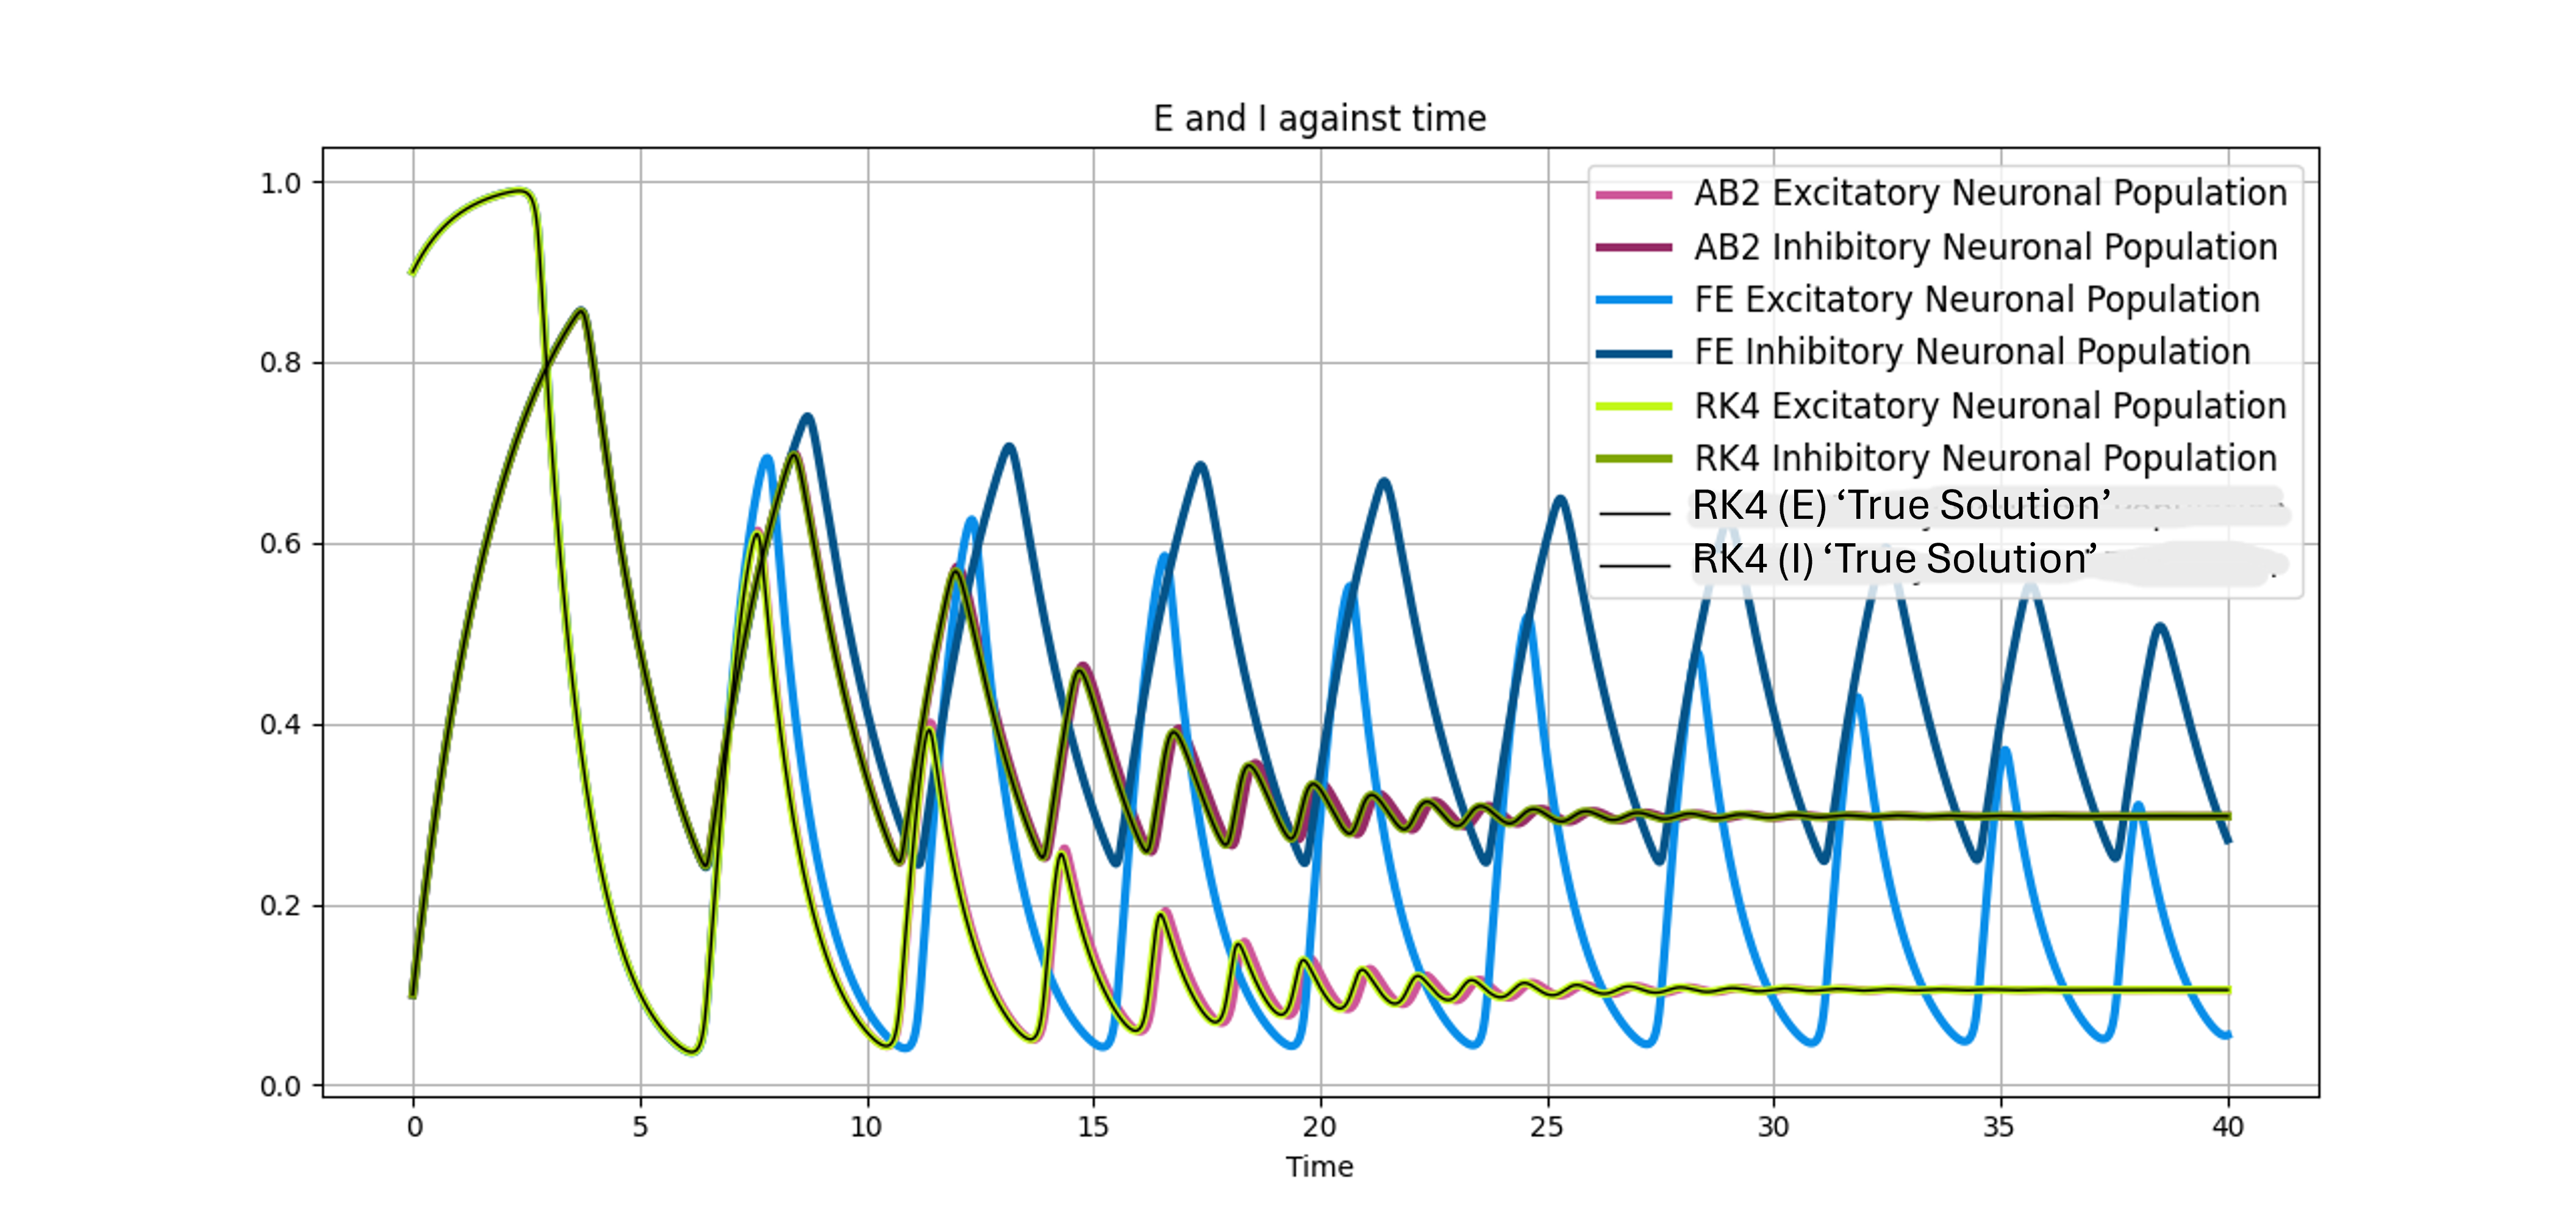
\includegraphics[width=\textwidth]{tashas graphs/damped comp.png}
    \caption{Comparison of methods when solving a damped oscillatory system}
    \label{fig:comparison of methods}
\end{figure}

We can compare how effective different numerical methods are at solving the Wilson-Cowan equations by considering the difference between the numerical solution and the true solution at each time step. We have compared the three numerical methods, Forward Euler, Fourth order Runge-Kutta and Adams-Bashforth. The forward Euler method is a first order method meaning that the local truncation error is $O(h)$ where h is the time step. The fourth order Runge-Kutta method is a fourth order method so the local truncation error is given by $O(h^4)$. Finally, the Adams-Bashforth method used is a second order method so has local truncation error is $h(O^2)$. Figure \ref{fig:comparison of methods} shows the numerical solutions to the Wilson-Cowan equations with initial conditions shown in table 3, using all three of the numerical methods with a time step of 0.01. We have assumed that the RK4 method will be the most accurate so we have mimicked the true solution by  using the fourth order Runge-Kutta with a very small time step of 0.0001. From this graph we can see that the forward Euler method deviates from the true solution much greater than the other two methods, therefore the forward Euler method is the least accurate. It can be seen that the Adams-Bashforth method and the fourth order Runge-Kutta method both produce a similar solution to the true solution. We can then plot the errors for each of the methods by considering the difference between the numerical solutions and our true solution at each time step. Figure \ref{fig:error comp} shows the error of the excitatory and inhibitory's progression over time from the decaying oscillations parameter values, for all three of the numerical methods. From this graph we can see that for both the E and I populations the error for the RK4 method is significantly lower than the error for the Forward Euler and the Adams-Bashforth methods which solidifies our assumption that the RK4 method is the most accurate at solving the Wilson-Cowan equations. 

\begin{figure}[h]
    \centering
    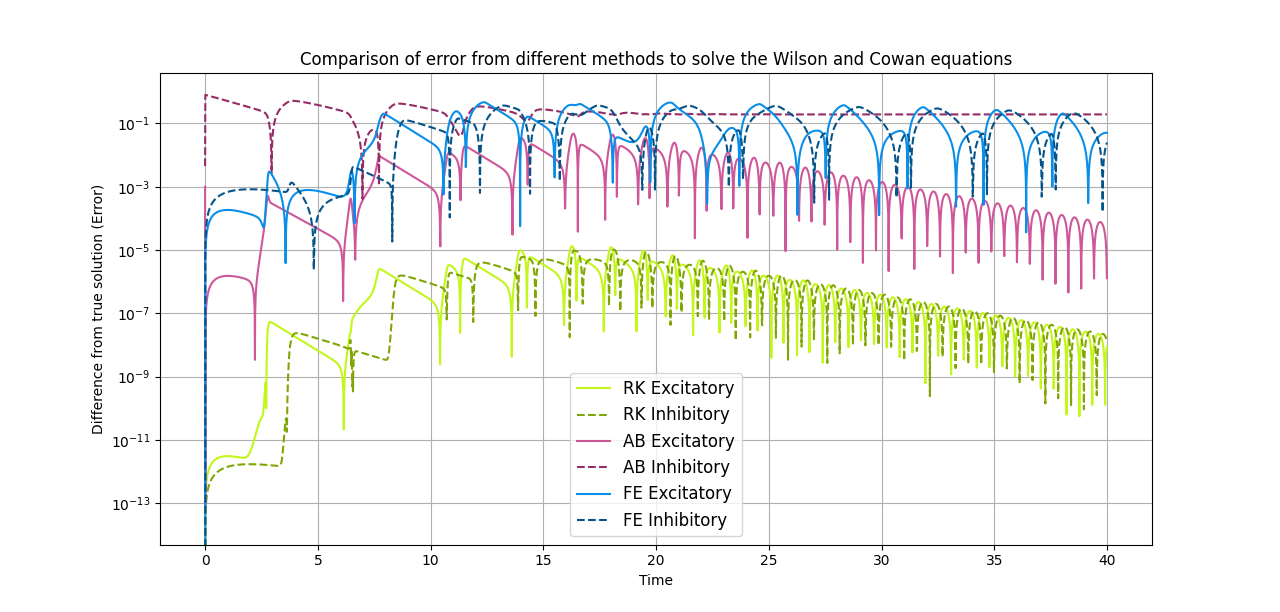
\includegraphics[width=\textwidth]{tashas graphs/damped error.png}
    \caption{Comparison of methods' error}
    \label{fig:error comp}
\end{figure}


\subsection{Numerically Solving the Model}

The Runge-Kutta method can be used to numerically solve the Wilson-Cowan model for a range of parameter values to find the dynamics of the neuron populations. We have chosen three sets of parameters and initial conditions to demonstrate the different behaviours of the Wilson-Cowan model. For each case, a graph can be plotted of the Excitatory (E) and Inhibitory (I) neuron values against time to visualise their behaviour. We calculated nullclines by solving $\frac{dE}{dt}=0$ and $\frac{dI}{dt}=0$, and then plotted these on a phase portrait of E against I with streamlines.

\subsubsection*{Stable Case}

The parameters and initial E and I conditions given by Table \ref{bif} produce a stable equilibrium point. The progression of the E and I neurons shown in Figure \ref{fig:stable only} follow a stable behavioural pattern as they are both seen to converge to a specific solution, which represents a state of balance within the neural network. Within the model, this stationary state could represent a stable equilibrium where the population dynamics are not specifically influenced by external stimuli \cite{wiki}. By plotting a phase portrait, this stable point can be visualised at the intersection point of the E and I nullclines. Interestingly, these parameters create a bifurcation where different initial E and I values cause the system to converge to different points. This can be seen in Figure \ref{fig:stable nullclines} as there are multiple intersection points of the nullclines and the streamline arrows point towards two of these points.

\begin{table}[h] 
    \centering
    \begin{tabular}{|c|c|c|c|c|c|c|c|c|c|c|c|c|}
    \hline
    Parameter & Initial E & Initial I & $\tau_E$  & $\tau_I$ & $\omega_{EE}$ & $\omega_{EI}$ & $\omega_{IE}$ & $\omega_{II}$ & P & Q & a & $\theta$ \\
    \hline 
    Values & 0.9 & 0.1 & 1 & 2 & 15 & 25 & 5 & 10 & 0 & 0 & 5 & 0 \\
    \hline
     \end{tabular}
     \caption{Parameter values for stable points}
     \label{bif}
\end{table}


\begin{figure}[!h]
    \centering
    \caption{Stable case}
    \begin{subfigure}[b]{0.48\textwidth}
        \centering
        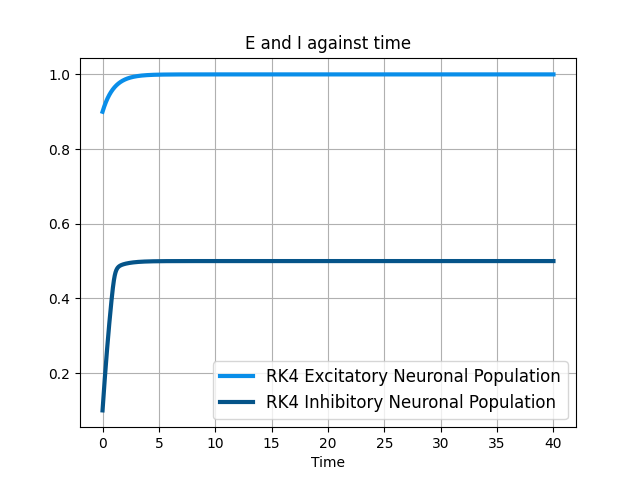
\includegraphics[width=\textwidth]{tashas graphs/stable only.png}
        \caption{Progression of E and I populations over time}
        \label{fig:stable only}
    \end{subfigure}
    \hfill
    \begin{subfigure}[b]{0.48\textwidth}
        \centering
        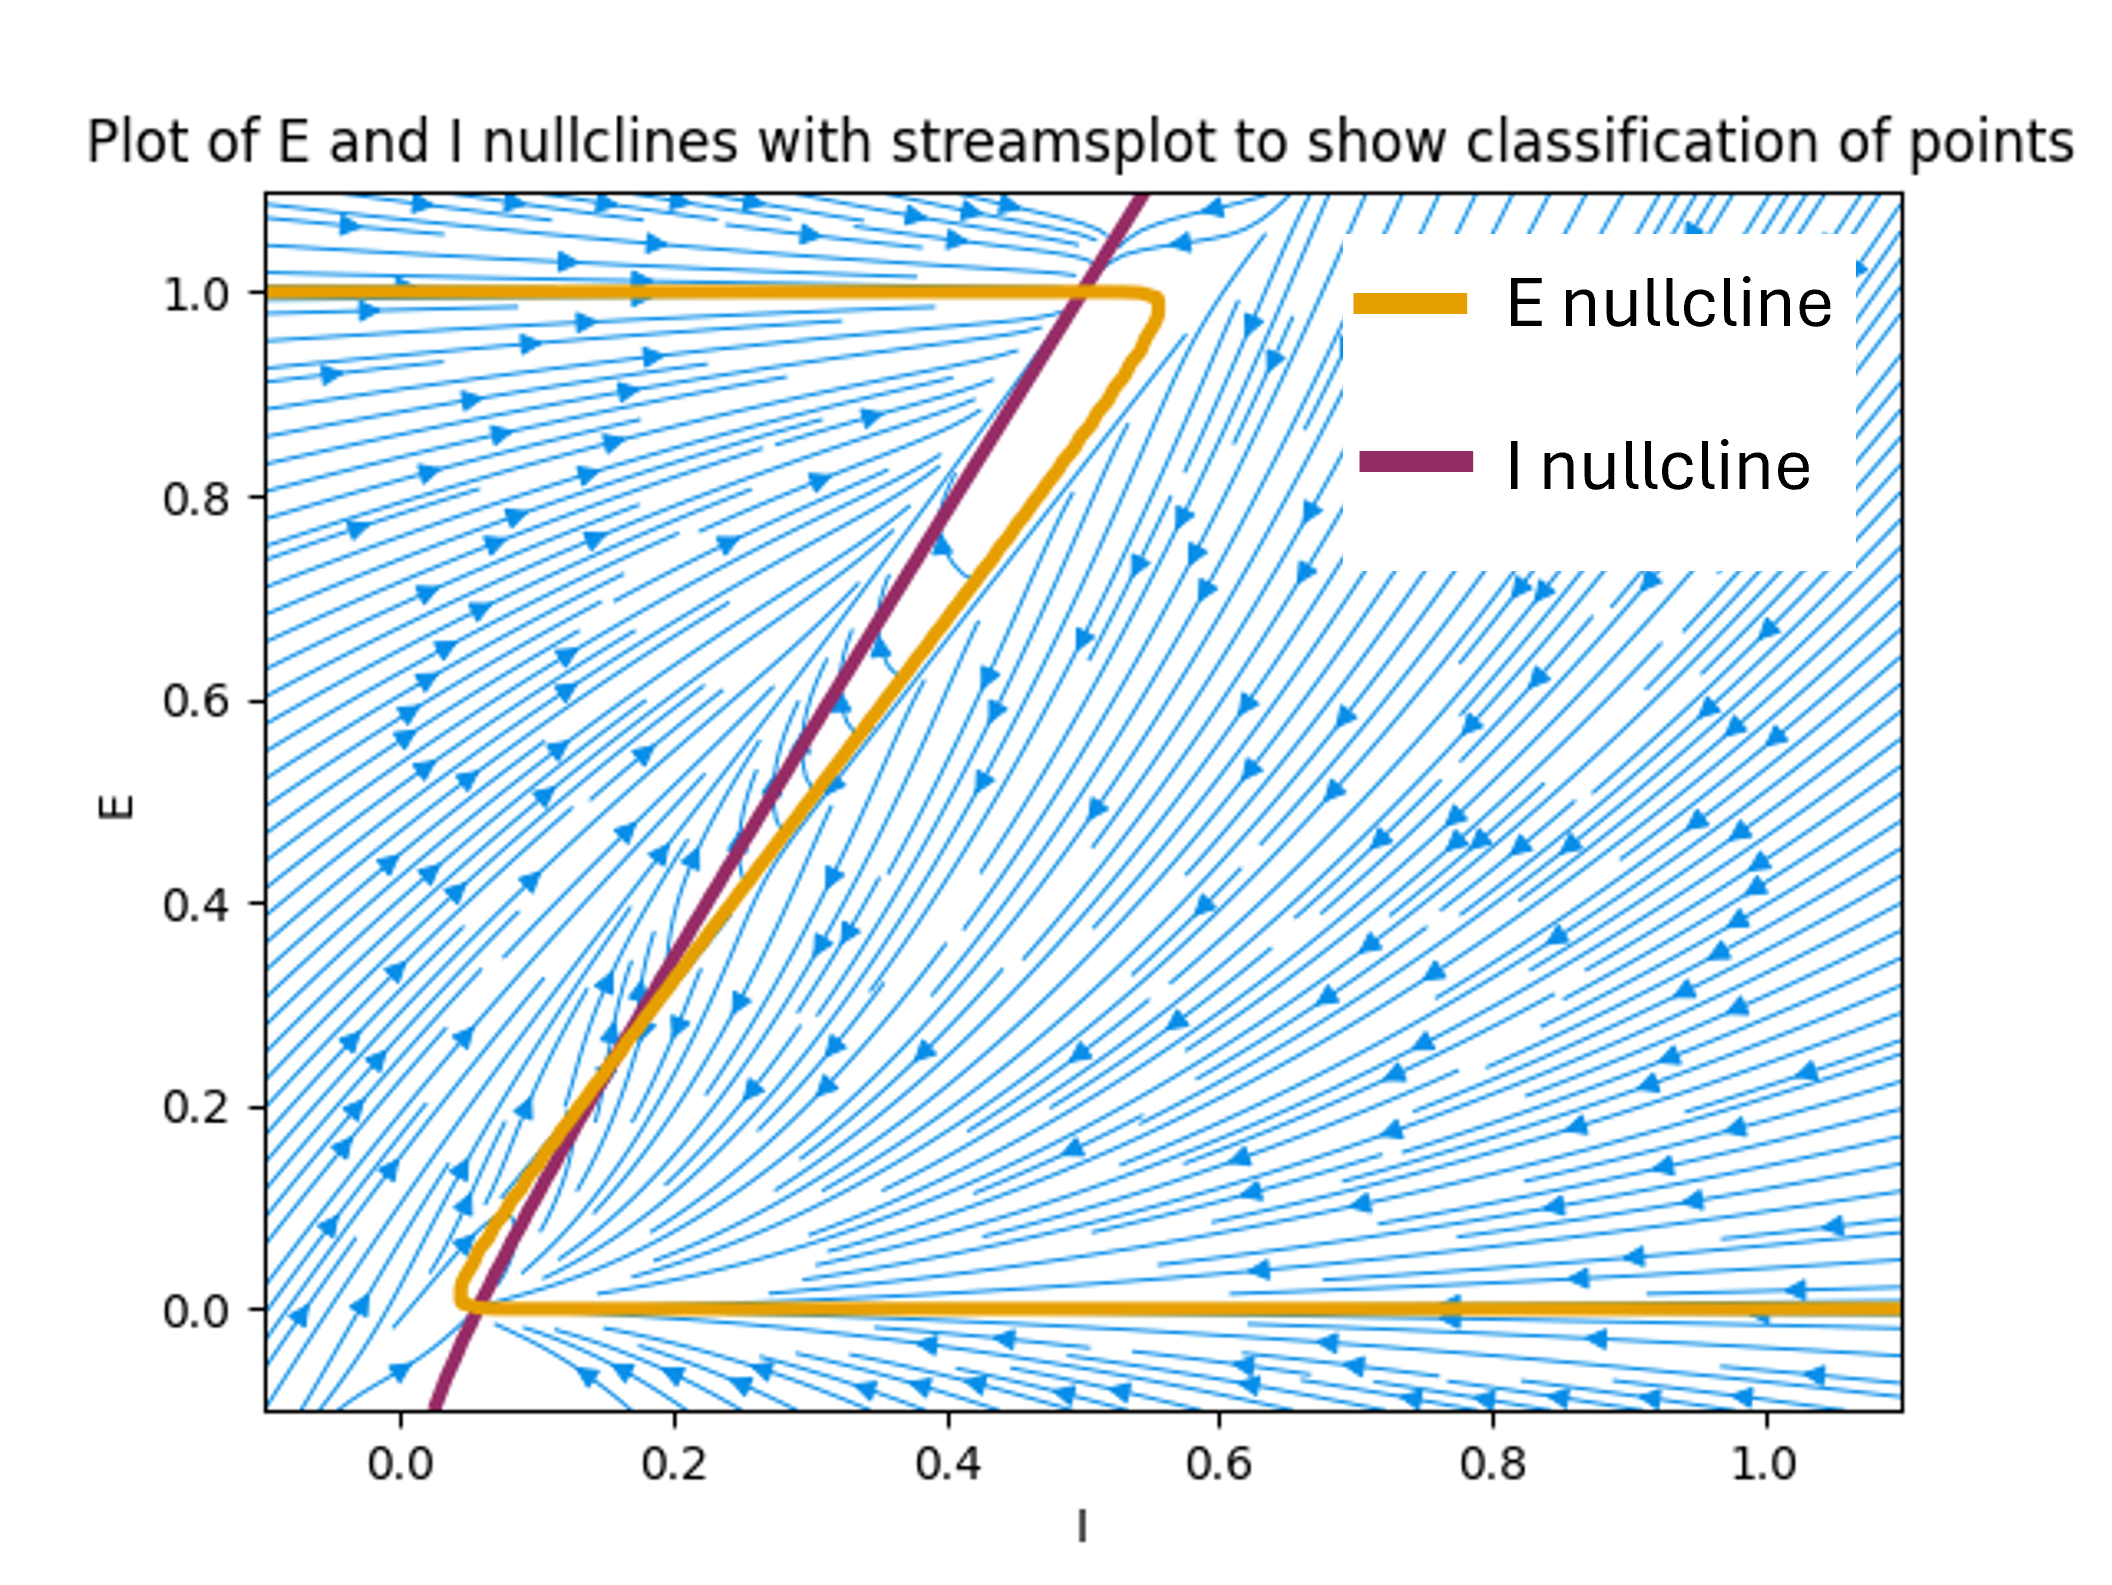
\includegraphics[width=\textwidth]{tashas graphs/stable nullclines.png}
        \caption{Phase Portrait}
        \label{fig:stable nullclines}
    \end{subfigure}
    \label{fig:stable}
\end{figure}

\subsubsection*{Sustained Oscillatory Case}

The parameters and initial E and I conditions given by Table \ref{Osc} produce an oscillatory point that does not converge to a solution. It can be observed in the progression of the E and I neurons shown in Figure \ref{fig:osc only} that the populations do not appear to converge over time and instead they both continue to oscillate, never reaching a state of equilibrium. This shows the model is producing oscillatory behaviour and can indicate that the model parameters are set to allow for multiple stable state and hysteresis in the population response. The oscillations represent the models ability to maintain activity levels, this can be observed in many applications, such as working memory simulations \cite{WC}. This behaviour can also be seen in Figure \ref{fig:osc nullclines} where the streamlines create a centre around the intersection point of the nullclines, rather than converging to this point like for the stable case.


\begin{table}[h] 
    \centering
    \begin{tabular}{|c|c|c|c|c|c|c|c|c|c|c|c|c|}
    \hline
    Parameter & Initial E & Initial I & $\tau_E$  & $\tau_I$ & $\omega_{EE}$ & $\omega_{EI}$ & $\omega_{IE}$ & $\omega_{II}$ & P & Q & a & $\theta$ \\
    \hline 
    Values & 0.1 & 0.9 & 1 & 2 & 15 & 25 & 25 & 10 & 5 & 0 & 5 & 0 \\
    \hline
     \end{tabular}
     \caption{Parameter values for oscillations}
     \label{Osc}
\end{table}

\begin{figure}[!h]
    \centering
    \caption{Sustained oscillations case}
    \begin{subfigure}[b]{0.48\textwidth}
        \centering
        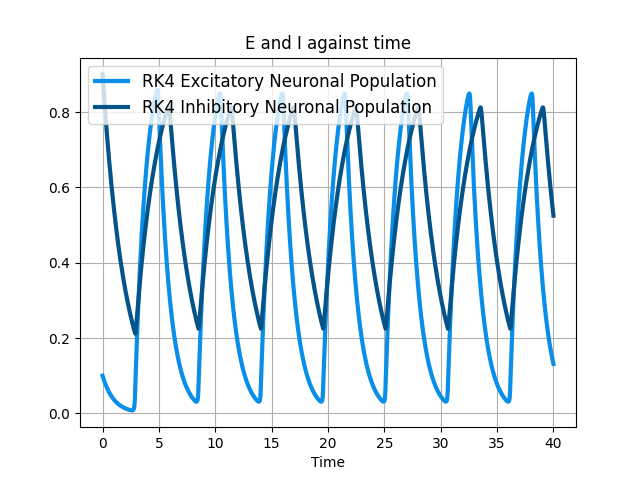
\includegraphics[width=\textwidth]{tashas graphs/osc only.png}
        \caption{Progression of E and I populations over time}
        \label{fig:osc only}
    \end{subfigure}
    \hfill
    \begin{subfigure}[b]{0.48\textwidth}
        \centering
        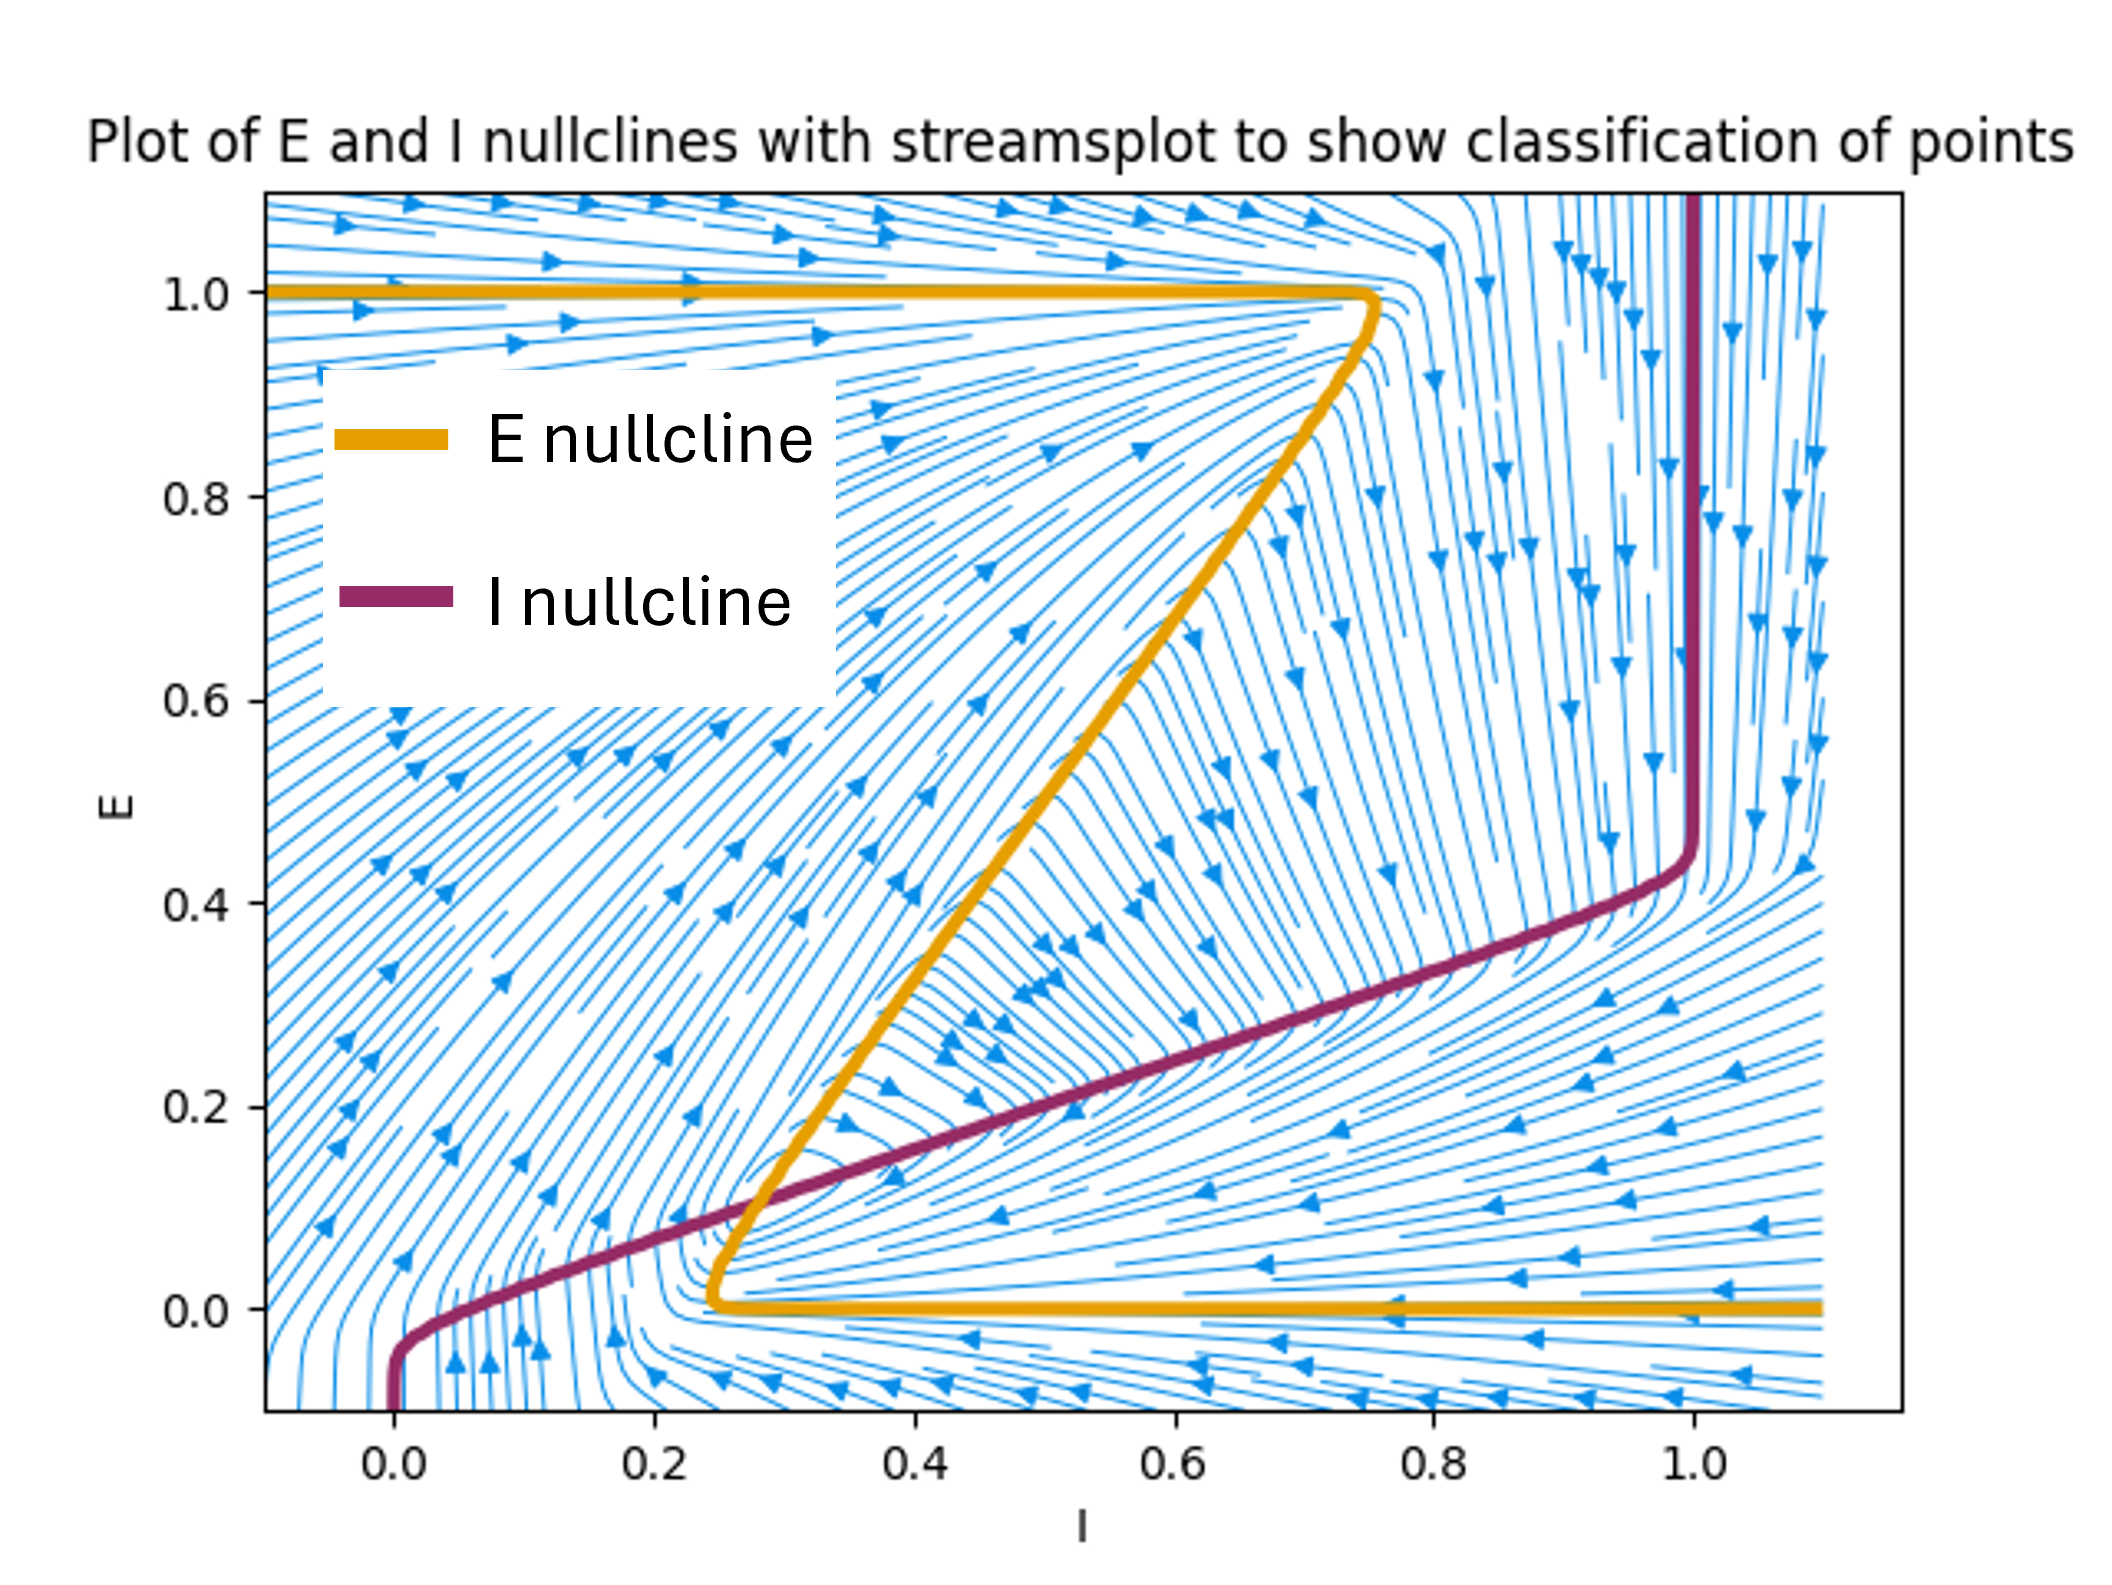
\includegraphics[width=\textwidth]{tashas graphs/osc nullclines.png}
        \caption{Phase Portrait}
        \label{fig:osc nullclines}
    \end{subfigure}
    \label{fig:osc}
\end{figure}

\subsubsection*{Decaying Case}

Finally, the parameters and initial E and I conditions given by Table \ref{Dam} produce a decaying oscillatory point that eventually converges to a solution (damped oscillations). The decaying oscillations show in Figure \ref{fig:damped only} indicate that the system's activity is not sustained over time and tends to return to a stable state. The damping effect of the oscillations prevents the activity from exhibiting chaotic behaviour and maintains stability. Decaying gamma oscillations are significant for understanding the dynamics of neural populations and their role in many brain functions, including decision making and sensory processing \cite{oscillation}. Figure \ref{fig:damped nullclines} shows the oscillations converging to the intersection point between the nullclines, compared to the previous (oscillatory) case which continued to circle the point without convergence or divergence.

\begin{table}[h] 
    \centering
    \begin{tabular}{|c|c|c|c|c|c|c|c|c|c|c|c|c|}
    \hline
    Parameter & Initial E & Initial I & $\tau_E$  & $\tau_I$ & $\omega_{EE}$ & $\omega_{EI}$ & $\omega_{IE}$ & $\omega_{II}$ & P & Q & a & $\theta$ \\
    \hline 
    Values & 0.9 & 0.1 & 1 & 2 & 15 & 25 & 25 & 10 & 5 & 0 & 2.5 & 0 \\
    \hline
     \end{tabular}
     \caption{Parameter values for decaying oscillations}
     \label{Dam}
\end{table}

\begin{figure}[!h]
    \centering
    \caption{Decaying oscillations case}
    \begin{subfigure}[b]{0.48\textwidth}
        \centering
        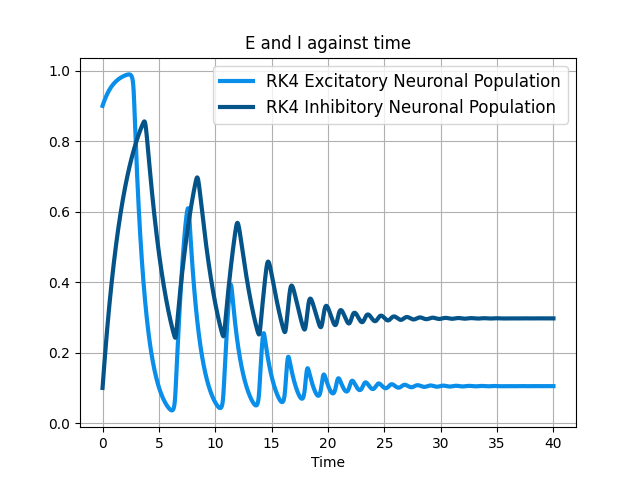
\includegraphics[width=\textwidth]{tashas graphs/damped only.png}
        \caption{progression of E and I populations over time}
        \label{fig:damped only}
    \end{subfigure}
    \hfill
    \begin{subfigure}[b]{0.48\textwidth}
        \centering
        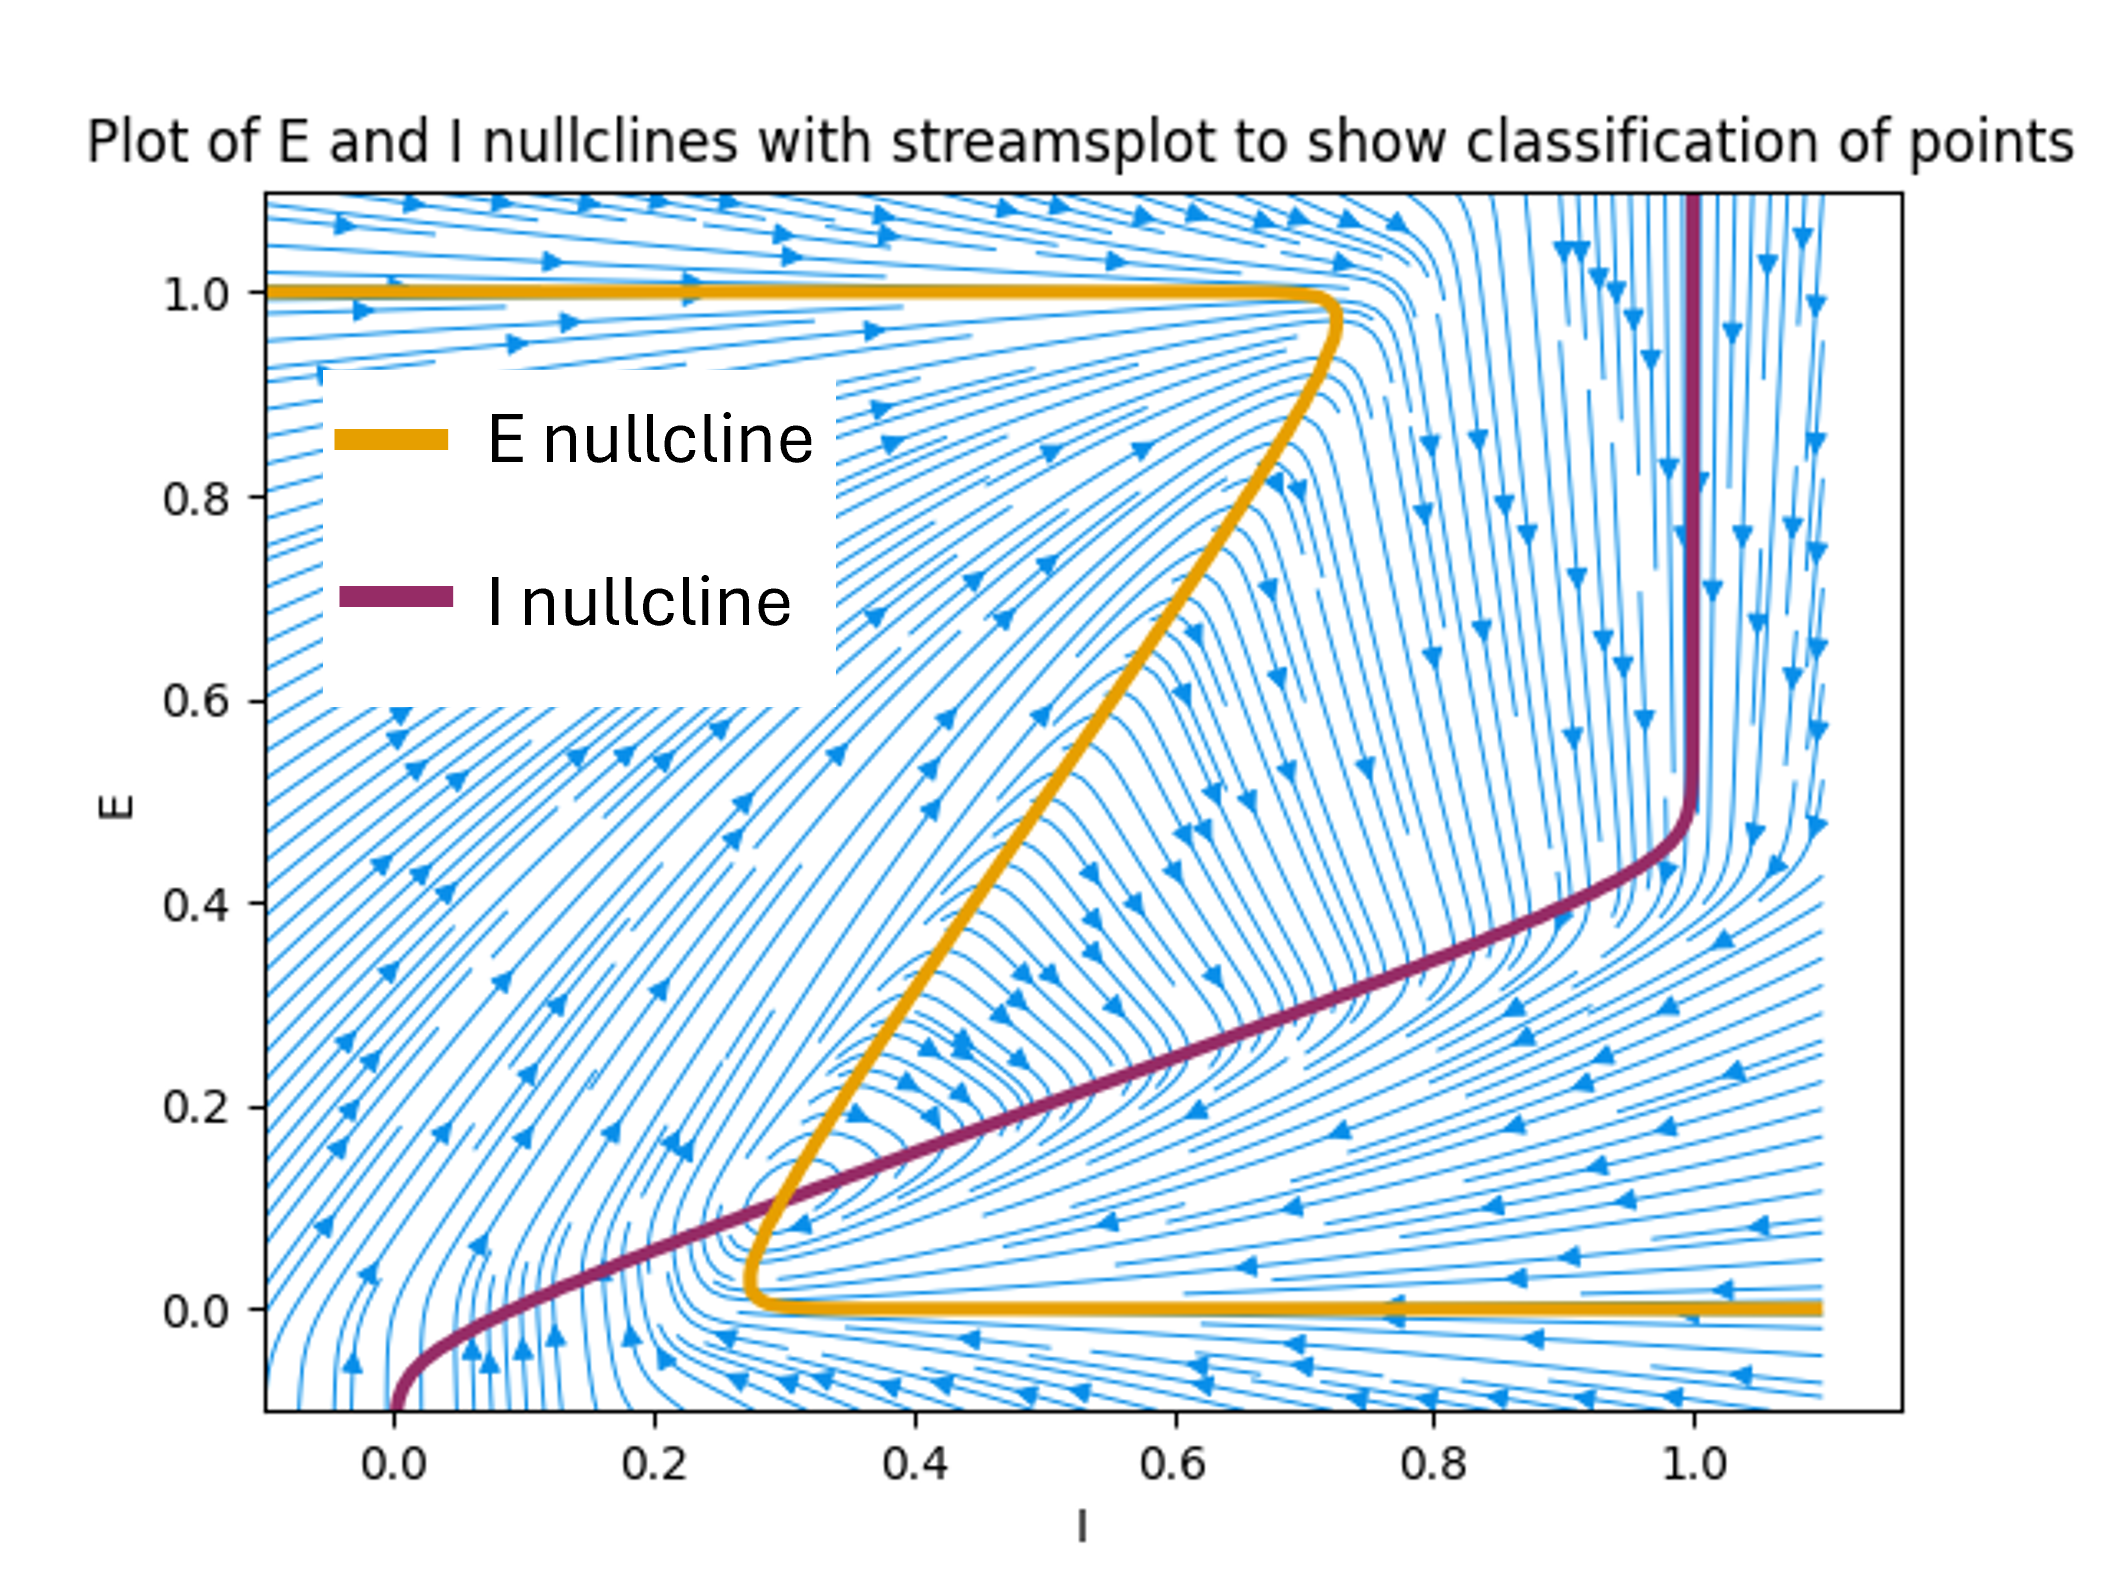
\includegraphics[width=\textwidth]{tashas graphs/damped nullclines.png}
        \caption{Phase Portrait}
        \label{fig:damped nullclines}
    \end{subfigure}
    \label{fig:damped}
\end{figure}



\begin{flushleft}

\section{Studying behaviour}

\subsection{Method}

We can study the behaviour of the Wilson-Cowan equations by putting a wide range of parameters through the Runge-Kutta method and analysing the corresponding behaviour from the model. We found a set of parameter values that gave sustained oscillations, then changed one parameter at a time and studied the effects on the behaviour of the model. This allowed us to infer the effect each parameter has on the whole model, however, this doesn't allow us to see how parameters interact with each other or how they work together to change certain behaviours.

\subsubsection{Choosing Parameters for initial sweep}

$E$ and $I$ represent the proportion of excitatory and inhibitory neurons that are active, so $E$ and $I$ will always be between $[0, 1]$. We chose to study $E$ and $I$ at $0.1$ and $0.9$, as it is important to sweep high and low initial conditions to test for bistability. $\tau_E$ and $\tau_I$ are time constants and, when considering shape and behaviour, the ratio of these is what effects the model, not their actual values. The fixed points characterised by negative values of $\tau_I$ or $\tau_E$ are repulsive and not relevant to the dynamics of the system\cite{journal} so, we kept the value of $\tau_E$ as 1 and explored ratios of $1:1$ and $1:2$. Studying one value of $\tau_E$ instead of two means the number of combinations of parameters will halve, so the parameter sweep will take half as much time and computing power. However, this means that the simulated time passed will not be an accurate representation of real life; in the original Wilson-Cowan paper\cite{hi}, they chose the time constants to be about 10 msec. "This value is in the range for the delays associated with the propagation of postsynaptic potentials from the dendrites of a neuron to the axon hillock (Oshima, 1969)"\cite{Oshima}.
\newline

Biologically, coupling strengths cannot be negative and $\omega_{EI}$ and $\omega_{IE}$ cannot be zero; this would mean $E$ and $I$ would not be interacting and the equations would no longer be coupled. In the original Wilson-Cowan paper\cite{hi}, $\omega_{EE}, \omega_{EI}, \omega_{IE}$ and $\omega_{II}$ are between 2 and 20 and values of $\omega_{II}$ are usually chosen to be lower than those of $\omega_{EE}, \omega_{EI}, \omega_{IE}$. In another paper \cite{gov}, $\omega_{EE}$ is also lower than $\omega_{EI}, \omega_{IE}$. We swept parameters in concurrence with these trends: $\omega_{EE} \in [0, 7, 15]$, $\omega_{EI} \in [5,15,25]$, $\omega_{IE} \in [5,15,25]$, $\omega_{II} \in [0,5,10]$.
\newline

In the published Wilson-Cowan paper\cite{hi}, $P = Q = 0$ is used most of the time and in a different article \cite{gov}, only positive input values were used. We swept parameters $P$ and $Q \in [0, 5]$.
\newline

Wilson and Cowan\cite{hi} and the other paper we read\cite{gov} use higher values of $\theta$ than $a$, usually keeping $a$ below 5 and b below 20. They also used different values of $a$ and $\theta$ in the inhibition and excitation sigmoids, but we did not, as it would make the parameter sweep take 6 times as long. $a$ cannot be 0 because then the sigmoid would provide an output of 0.5 no matter the input, which is not useful for modelling interactions of $E$ and $I$. However, $\theta$ can be zero and still allow model to function, so we tested it out of interest. We swept parameters $a \in [1, 5]$ and $\theta \in [0,5,20]$
\newline

\subsubsection{Behaviour}

Each regime is either stable or has repeating oscillations; if it's stable, $E$ and $I$ either converge straight to equilibrium, or enter a state of decaying oscillations that die out as the system reaches equilibrium. If the system exhibits no oscillations, it is classed as "straight to stable". If the amplitude of oscillations is shown to decrease over time, the regime is classed as "decaying oscillations". If oscillations maintain amplitude across the whole time-frame, regime is classed as "sustained oscillations". 
\newline

We calculated the mean activity of $E$ and $I$ in the last half of the time we ran the Runge-Kutta scheme for. This is so any short term behaviour, such as large fluctuations or rapid increases to a steady state in the transient period, would not skew our value for the mean of long term, steady state behaviour. However, if decaying oscillations continued out of the first half of the measured time period, these could skew the mean. But any oscillations would be around the equilibrium state, so mean activity should still be reasonably accurate. The only outlier for this assumption would be if frequency is so small that the time isn't long enough to display a full oscillation, which would mean $E$ or $I$ would only be shown to be in a high or low activity state, making the mean much higher or lower than the true average activity.
\newline

We also calculated the maximum amplitude of oscillations as opposed to the average amplitude of oscillations; a series of decaying oscillations that starts with a high amplitude but dies away fast could have the same average amplitude of oscillations as a regime that started with half the amplitude of oscillations but dies away very slowly. This means it is more useful for us the measure the maximum amplitude. We looked at amplitude of oscillations over the last half of the time we ran the Runge-Kutta method for when looking at sustained oscillation, so that any larger oscillations in the transient period were excluded. However, for the decaying oscillation cases, we looked at the maximum amplitude over the whole time. Due to the fact that we measured over different periods of time for different regimes, we can only compare within the same regime, however, this can still provide useful information on the behaviour of the model.
\newline

We measured the frequency of oscillations of $E$ and $I$ over the entire time, however, this calculation is not very useful when studying the behaviour of decaying oscillations. If $E$ and $I$ don't oscillate over the entire time period, the calculated frequency will be much lower than the actual frequency of oscillations. Because of this, we will not discuss how varying parameters affect frequency of oscillations in a regime classified as decaying oscillations.
\newline

We also checked for bistability; if different initial conditions lead to different equilibrium means, there are two or more equilibrium points the system could converge to in the phase space. 
\newline


\subsection{Varying parameters}

We observed how changing each parameter individually affected frequency and amplitude of oscillations, mean of $E$ and $I$ at equilibrium and regime classification. We calculated these for 9 sets of initial conditions: $E \in [0.1,0.5,0.9]$ and $I \in [0.1,0.5,0.9]$. In most cases, changing the initial conditions did not affect results, so only graphs displaying changes for initial conditions $E=0.1$ and $I=0.1$ are displayed in the appendix. Any special cases are discussed individually.

\subsubsection{The Sigmoid Function}

The sigmoid function is given as:

\[
\phi (x) = \frac{1}{1+e^{-a(x-\theta)}}
\]

It is an S-shaped function that converts an input (either $x = \omega_{EE}E - \omega_{EI}I + P \quad \text{or} \quad \omega_{IE}E - \omega_{II}I + Q$)
into an output between 0 and 1. In the Wilson-Cowan model, the sigmoid represents how strongly the neural population responds to small changes in $E$ and $I$.
\newline
When $x << \theta$, the exponent, $-a(x -\theta)$, is large and positive, so $\phi$ is close to 0. When $x>> \theta$, the exponent is large and negative, so $\phi$ is close to 1. When $x=\theta$, $\phi = 1/2$ so $\theta$ represents the "threshold value". Since the sigmoid function is "s-shaped", the output changes rapidly when $x$ changes near the threshold, and barely changes when $x$ is much lower or higher than $\theta$. When $\theta$ is higher, $x$ must also be higher to enter a "higher activity" state i.e. the sigmoid producing large outputs. This means that the $E$ and $I$ populations are harder to activate. The parameter $a$ controls the steepness of the slope of the sigmoid, which corresponds to how sharply the populations of $E$ and $I$ respond to small changes.

\subsubsection{$a$}

\begin{flushleft}
As shown in figure \ref{a graphs}, when $a \leq 2.5$  the response to changes in $E$ and $I$ are gradual so, if $E$ or $I$ overshoot equilibrium, they can be corrected before they rise too much, so oscillations will die away. As $a$ increases, the sigmoid produces a steeper output, so $E$ and $I$ will rise faster. This means that the populations respond more abruptly to each other, which allows the oscillations to be sustained. In sustained oscillations, the population of $E$ rising faster means it gets higher before inhibition suppresses it, so amplitude of oscillations of $E$ will increase. This in turn increases the amplitude of oscillations of $I$. But if $E$ and $I$ are spending longer in excited states, the oscillation period increases, so the frequency of oscillations decreases. Changing $a$ does not directly affect the mean activity of $E$ and $I$, but the frequency and amplitude of oscillations have contrasting effects on the equilibrium mean, so it's affected non-monotonically as $a$ increases.
\end{flushleft}

\begin{flushleft}
Trying to set $a \geq 35$ leads to a python exponential overflow warning, so we didn't explore the effects of a being higher than this.
\end{flushleft}
\subsubsection{$\theta$}

In figure \ref{b graphs} $\theta$ is represented as $b$. When $\theta \leq -1.67$, the threshold of the sigmoid is low, so most changes in $E$ and $I$ occur above the threshold, so the sigmoid responds very little to changes in input. This means any oscillations will decay quickly as $E$ and $I$ don't respond strongly to each other. Within these decaying oscillations, as $\theta$ increases, $E$ and $I$ need to be higher to cause the sigmoid to give the same output. Therefore, equilibrium means of $E$ and $I$ fall as the sigmoid function is contributing less to the rise of $E$ and $I$. However, if the mean activity of inhibition is falling, excitation is suppressed less. The effect of less suppression on the population of $E$ is stronger than direct effect of $\theta$ on $E$ so the mean activity of $E$ increases.
\newline

When $\theta$ increases further, changes in $E$ and $I$ will be nearer the threshold, so the sigmoid function is sensitive to small changes, inducing sustained oscillations. When $\theta$ is still low in the range that allows sustained oscillations, frequency increases with $\theta$, because the threshold value is getting closer to where the changes in input are occurring due to oscillations of $E$ and $I$ around the equilibrium point. This means the sigmoid function responds more to changes in $E$ and $I$, so the system can switch from excitation to inhibition faster, increasing frequency. When $\theta$ increases more, the threshold is higher than where the input is fluctuating, so the sigmoid responds less to changes in $E$ and $I$. This means the system switches from excitation to inhibition slower, decreasing frequency. Increasing $\theta$ within the regime of sustained oscillations has the same effect on the means of $E$ and $I$ as in decaying oscillations, but the effect of less suppression on the population of $E$ is weaker than direct effect of $\theta$ on $E$, so the mean of $E$ decreases, but at a slower rate than the mean of $I$. The means of $E$ and $I$ are also affected by frequency: because this changes non-monotonically, the means of $E$ and $I$ also decreases non-monotonically. $\theta$ does not directly affect the amplitude of oscillations of $E$ and $I$, so this is affected by the change in frequency and equilibrium means. As before, these changes are not monotonic so neither are the changes in amplitude of oscillations. However, there is an overall decrease in amplitude of sustained oscillations as $\theta$ increases. This is likely due to the fact that the means of $E$ and $I$ are decreasing, so the sigmoid is receiving less input, so contributing less to the rise of $E$ and $I$.
\newline

When $\theta \geq 6.33$, all inputs are below the threshold, changes in $E$ and $I$ have no effect on the output of the sigmoid function, so no oscillations occur. 

\subsubsection{$\tau_I$}

When $\tau_I \leq$ 1.53, the speed at which $I$ responds to an increase in $E$ is fast enough that $E$ is suppressed before it overshoots and causes oscillations. Therefore, the regime is stable. $\tau_I$ only has an affect on the timing of inhibition, so does not have an effect on the mean activity of $E$ and $I$ in stable regimes.
\newline

When $\tau_I \geq 1.6$, the system shows sustained oscillations, since $I$ responds respond slow enough that $E$ has a chance to build up and overshoot before being suppressed. $I$ is influenced by $E$ through $\omega_{IE}E$, so this overshoot also causes $I$ to overshoot, causing oscillations. Increasing $\tau_I$ does not change the regime from sustained oscillations, since $I$ will eventually respond to the rise in $E$ even if it takes longer, which only reduces the frequency of oscillations, doesn't stop them. This also means that $E$ can rise further before it's inhibited, so the amplitude of oscillations of $E$ are higher. $I$ then rises higher to inhibit $E$, so the amplitude of oscillations of $I$ will also increase. $E$ having more time to grow before it's inhibited means that the mean activity of $E$ also increases, as it spends longer in a high activity state. This also causes the mean activity of $I$ to increase, as $I$ is driven by $E$ due to the $\omega_{IE}E$ term. However, the mean activity of $E$ and $I$ is also affected by the amplitude and frequency of oscillations. These have different effects of the means of $E$ and $I$ so the combination of these effects leads to a non-monotonic increase, as shown in figure \ref{TI graphs}.


\subsubsection{$\omega_{EE}$}

\begin{flushleft}
    In Figure \ref{WEE graphs}, we can see that when $\omega_{EE} \geq 12.5$, $E$ excites itself enough that a small increase in $E$ causes a large rise in activity, so $E$ overshoots equilibrium. This causes a significant rise in $I$ to correct the overshoot. This process repeats, causing sustained oscillations. When $\omega_{EE}$ increases, $E$ rises more for the same small change in its population. A larger rise in $E$ increases the amplitude of oscillations of $E$. This, in turn, increases the amplitude of oscillations of $I$. Because $E$ and $I$ spend longer in high activity states, the oscillation loop takes longer to complete, decreasing frequency of oscillations.
    \newline
    
    When $\omega_{EE} \leq 12$ the population of excitatory neurons aren't exciting themselves enough, so $E$ rises slower. This means that $E$ doesn't overshoot the equilibrium by much before the population is suppressed, so oscillations decay and $E$ and $I$ reach a steady state. As $\omega_{EE}$ increases, $E$ rises further, increasing amplitude of oscillations, so $E$ stays in a high activity state longer. This increase the mean activity of $E$. $I$ then rises further to suppress the higher activity levels of $E$, increasing the amplitude of oscillations of $I$. This means the inhibitory population stays in a high activity state for longer, increasing the mean activity of $I$.
    \newline
    
    When $\omega_{EE} \geq 21.5$ the population of excitatory neurons excite themselves so strongly that they cannot be suppressed by inhibition. This means $E$ continues to rise until the whole population is firing, so its mean activity is 1. $I$ also continues to rise until its whole population is firing, because it is driven by the $\omega_{IE}E$ term, so its mean activity will also be 1. The activity of $E$ and $I$ exhibit no changes after this state is reached so the regime is stable.
\end{flushleft}


\subsubsection{$\omega_{EI}$}

Increasing the value of $\omega_{EI}$ strengthens the effect of inhibition on the excitatory population. When $\omega_{EI} \leq 18.3$, $I$ does not have a strong inhibitory effect on the activity of $E$, so $E$ rises until the entire population is firing. $I$ also rises due to the $\omega_{IE}E$ term, and also reaches a stable state when the entire population is firing. This is shown in figure \ref{WEI graphs}: mean activity of $E$ and $I$ is 1, and the regime is stable.
\newline

When $\omega_{EI} \geq 19$, $I$ inhibits $E$ enough that $E$ falling when $I$ rises. This means the activity of $I$ will also fall, so the activity of $E$ will increase again, as it stops being inhibited. This cycle repeats, causing sustained oscillations. As $\omega_{EI}$ increases, $E$ is suppressed more strongly by $I$, so the peak activity level $E$ reaches is lower, and $E$ spends less time in a high activity state. This causes amplitude of oscillations and the mean activity of $E$ to decrease. Since $I$ is driven by $E$, the amplitude of oscillations and mean activity of $I$ also decreases. Increasing $\omega_{EI}$ means $E$ is inhibited more quickly, decreasing time taken for an oscillation to occur and increasing frequency.
\newline

When $\omega_{EI} \geq 30.3$, $I$ suppresses $E$ so strongly that $E$ cannot rise enough to sustain oscillations. Oscillations decay until a stable state of $E$ and $I$ is reached. As $\omega_{EI}$ increases within this regime, amplitude of oscillations decreases as $E$ is rises to lower peaks. This also means that oscillations will die out faster, meaning less will occur over out calculated time, reducing the displayed frequency value.

\subsubsection{$\omega_{IE}$}

\begin{flushleft}
When $\omega_{IE} \leq 7.5$, an increase in $E$ does not cause a large increase in $I$. $I$ then doesn't inhibit the increase in $E$, so $E$ rises until the entire population is firing, which gives mean activity of 1. As $\omega_{IE}E$ increases, $I$ is affected more strongly by the high activity level of $E$; mean activity of $I$ will increase as shown in figure \ref{WIE graphs}.
\newline

When $\omega_{IE} \geq 8.33$, an increase in $E$ causes a large enough increase in $I$ that $E$ is suppressed and falls. This means $I$ will also fall, so $E$ will increase again, as it stops being inhibited. This cycle repeats, causing sustained oscillations. As $\omega_{IE}$ increases, $I$ is driven more strongly by changes in $E$, so it rises to a higher level of activity, increasing the amplitude of oscillations and the mean activity level. This higher level of activity of $I$ means it spends longer in a high activity state, increasing the time for an oscillation to occur, decreasing frequency and mean activity of $E$. The contrasting effects of frequency and amplitude of oscillations mean that the effect of $\omega_{IE}$ on the mean activity of $E$ and $I$ is non-monotonic. However, the overall trend observed in figure \ref{WIE graphs} is that of the mean activity of $E$ decreasing and $I$ increasing.
\newline 

\end{flushleft}


\textbf{SPECIAL CASE}

At $\omega_{IE}=10$, the point around which the system is oscillating is exactly (0.5,0.5), as shown in the phase plot \ref{WIE = 10}. So for initial conditions $E = 0.5$, $I=0.5$, the system exhibits no change in behaviour, shown in \ref{Q = -7.5 timeseries}, contrary to the expectation of sustained oscillations; in \ref{WIE 0.5 0.5}, it doesn't make sense that the point $\omega_{IE}=10$ is would be at a stable node.

\subsubsection{$\omega_{II}$}

\begin{flushleft}

When $\omega_{II} \geq 5.2$, the inhibitory population suppresses itself enough that $E$ can rise before inhibition suppresses it. $E$ falls when inhibited, causing $I$ to fall, then causing $E$ to increase again as it stops being inhibited. This cycle repeats, causing sustained oscillations. Increasing $\omega_{II}$ means inhibitory response gets cut off very early and amplitude of oscillations of $I$ decrease. This makes whole whole oscillation loop shorter, so frequency of oscillations increases. Because $I$ reaches lower peak activity levels, $E$ rises further, increasing the amplitude of oscillations of $E$. However, the oscillations loop becoming shorter means that $E$ has less time to increase, so it reaches lower peak activity levels. These contrasting effects on the amplitude of oscillations of $E$ mean that as $\omega_{II}$ increases, the effect it has on the amplitude of oscillations of $E$ is non-monotonic. In every regime type, increasing $\omega_{II}$ means the average inhibitory activity will decrease. This means less overall inhibition acts on $E$, resulting into a higher mean excitatory activity. However, the mean activity of $E$ and $I$ in sustained oscillations is affected by the amplitude of frequency of oscillations too, so overall changes aren't monotonic.
\newline

When $\omega_{II} \leq 4.67$, the inhibitory population reacts quickly to any rise in $E$ , so any oscillations are damped and the system will decay to a steady state. As $\omega_{II}$ increases, the inhibitory response gets cut off faster, so the amplitude of oscillations of $I$ decrease and the whole oscillation loop becomes shorter. This means that $E$ has less time to increase, so it reaches lower peak activity levels, thus having lower oscillation amplitude.
\end{flushleft}

\begin{flushleft}
\textbf{SPECIAL CASE:} \\

In figure \ref{WII graphs 0.1 0.5}, $5.2 \leq \omega_{II} \leq 5.73$ show decaying oscillations, but other initial conditions, for example in \ref{WII graphs}, show sustained oscillations. The phase plots, shown figures \ref{WII = 5.2} and \ref{WII = 5.73}, clearly show a stable spiral, so this is likely a classification error caused by the amplitude of oscillations decreasing so slowly that the code misclassifies the regime as sustained oscillations. This could be resolved by running the code for longer, so the oscillations would have chance to decay more, or being stricter in the classification of sustained oscillatory regimes.
\end{flushleft}

\subsubsection{$P$}

In figure \ref{Q graphs}, when $P \leq 4$, the input to the excitatory sigmoid is far below the threshold, so changes in $E$ cause very weak oscillations. These are easily damped by $I$, so oscillations decay into a steady state.

When $P \geq 5$, the input to the excitatory sigmoid is near the threshold; the sigmoid reacts sensitively to changes in input, so $E$ rises rapidly. This causes $I$ to rise rapidly via the $\omega_{IE}E$ term, inhibiting $E$ and causing it to fall. $I$ then falls and stops suppressing $E$, allowing $E$ to rise again. This cycle repeats and sustained oscillations occur. Increasing the value of $P$ means that the population of $E$ is driven upwards more strongly, increasing amplitude of oscillations. $I$ must then also rise higher to suppress $E$, so amplitude of oscillations of $I$ also increases. When $P$ increases further, the sigmoid input becomes larger than the threshold and the population of $E$ stays at a higher baseline. The sigmoid becomes less sensitive to changes in the input so $E$ is driven to rise less strongly, decreasing amplitude of oscillations. $I$ then rises to lower peaks when suppressing $E$, so amplitude of oscillations of $I$ also decrease.
\newline

When $P \geq 5$ but still low, $E$ being driven upwards more strongly means it spends longer in a high activity state, increasing the amplitude of oscillations of $E$. This means $I$ has to stay in a higher activity state to suppress $E$, so amplitude of oscillations of $I$ also increases. This increases the time taken per each oscillation, so the frequency decreases. As the value of $P$ increases further, the excitatory population stays at a higher baseline value. This means the excitatory sigmoid becomes less sensitive to changes in input because the input is further above the threshold. This lowers the amplitude of oscillations of $E$ and $I$ and also means changes in $E$ occur more slowly, accelerating the effect of increasing the value of $P$ on the frequency.
\newline

When $P \geq 30$, the input to the excitatory sigmoid is well above the threshold, so any changes in $E$ population do not cause oscillations. $I$ does not inhibit $E$ strongly, as the excitatory sigmoid will produce a high output no matter the effect of the $\omega_{EI} I$ term. This mean that $E$ rises straight to its maximum level of activity, which also causes $I$ to do the same. This means $E$ and $I$ go straight to stable equilibrium of means 1 with no oscillations.


\subsubsection{$Q$}

In figure \ref{Q graphs}, when $Q \leq -16.67$, the input to the inhibitory sigmoid is far below the threshold, so changes in $I$ do not cause any oscillations, and $I$ remains low. This means that $E$ rises straight to equilibrium. 

When $Q \geq -15.83$, the input to the $I$ sigmoid is near the threshold; the sigmoid reacts sensitively to changes in $I$, so when $E$ rises and causes a small change in input via the $\omega_{IE}E$ term, $I$ increases rapidly and over-corrects the increase in $E$. This increase in $I$ causes an overshoot in $E$ via the $\omega_{IE} E$ term, causing the cycle to repeat and oscillations to occur. In a sustained oscillation regime, increasing $Q$ makes inhibition activate earlier. This means $E$ is inhibited sooner, so the amplitude of oscillations of $E$ falls and the oscillations cycle takes less time, increasing frequency. However, if the peaks of $E$ are not as high, $I$ will be less affected by $\omega_{IE}E$ term, reducing the amplitude of oscillations of $I$, which in turn, increases the amplitude of oscillations of $E$. In contrast, $I$ rising faster means it will reach a higher peak before falling, increasing the amplitude of oscillations of $I$. So, $I$ will spend longer in an active state, so the oscillation cycle will take longer, reducing frequency. These contradictions of the effects of changing $Q$ on the frequency and amplitude of oscillations means the changes are not monotonic. when $Q$ is very high, the input to the sigmoid is above the threshold value, so the system doesn't react strongly enough to changes in $I$ to sustain a large repeating oscillation. Any oscillations decay, and the trajectory returns to a stable steady state.
\newline

In all regime types, increasing $Q$ increases mean activity of $I$ and decreases mean of $E$. Increasing $Q$ directly increases $I$, so the mean activity of $I$ increases, while the excitatory population is suppressed more strongly, so the mean of $E$ decreases.
\newline

\textbf{SPECIAL CASE:} \\
At $Q = -7.5$, the point around which the system is oscillating is exactly (0.5,0.5), as shown in the phase plot \ref{Q = -7.5 streamplots}. So for initial conditions $E = 0.5$, $I=0.5$, system exhibits no change in behaviour, shown in \ref{Q = -7.5 timeseries}, contrary to the expectation of sustained oscillations; in \ref{Q 0.5 0.5}, it doesn't make sense that the point $Q=-7.5$ is classified as stable.

Also in figure \ref{Q 0.5 0.5}, $Q = 0.83$ and $Q = -15.833$ show decaying oscillations. Other initial conditions, for example in \ref{Q graphs} show sustained oscillations. The phase plots, shown in \ref{Q = -15.833 streamplot} and \ref{Q = 0.83 streamplot}, clearly show a stable spiral, so this is likely a classification error caused by the amplitude of oscillations decreasing so slowly that the code misclassifies the regime as sustained oscillations. This could be resolved by running the code for longer, so the oscillations would have chance to decay more, or being stricter in the classification of sustained oscillatory regimes.

\subsection{Bistability}

The code classifies a set of parameters as bistable if its means for different initial conditions are more than 5\% different. In sustained oscillations, how far through an oscillation cycle the system is when it's cut off will skew mean of $E$ and $I$. This means different initial conditions cause the curve to be cut off at different points so system will display different means, even though they should be the same as oscillations are around the same stable point in the phase plot \ref{fig:sustained-oscs-non-bistable-phase-plot}.

\begin{table}[!ht]
    \centering
    \begin{tabular}{|l|l|l|l|l|l|l|l|l|l|l|l|}
    \hline
        TE & TI & WEE & WEI & WIE & WII & P & Q & a & b & Mean of E at eq. & Mean of I at eq. \\ \hline
        1 & 2 & 15 & 25 & 25 & 10 & 5 & 0 & 2.666666667 & 0 & 0.159220501 & 0.385425819 \\ \hline
    \end{tabular}
    \caption{Parameters that give bistable regime}
\end{table}

Systems that are actually bistable are caused by the presence of two or more nodes in the phase plane e.g. figure \ref{fig:bistable-phase-plot}, and different initial conditions means the system can converge to any of them, leading to different means of $E$ and $I$ in stable state.

\begin{table}[!ht]
    \centering
    \begin{tabular}{|l|l|l|l|l|l|l|l|l|l|l|l|l|l|l|l|l|l|l|l|l|}
    \hline
        TE & TI & WEE & WEI & WIE & WII & P & Q & a & b & Mean of E at eq. & Mean of I at eq. \\ \hline
        1 & 1.666666667 & 15 & 25 & 25 & 10 & 5 & 0 & 5 & 0 & 0.26968477 & 0.489889758 \\ \hline
    \end{tabular}
    \caption{Parameters that give false bistable regime}
\end{table}

\begin{figure}[!h]
    \centering
    \begin{subfigure}[b]{0.48\textwidth}
        \centering
        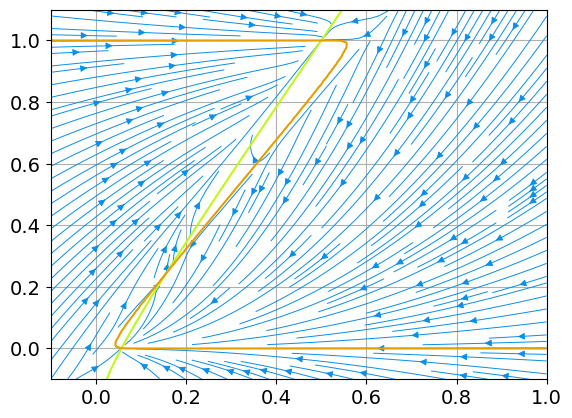
\includegraphics[width=\linewidth]{param graphs/bistable nullcline plot.png}
        \caption{Bistable phase plot}
        \label{fig:bistable-phase-plot}
    \end{subfigure}
    \hfill
    \begin{subfigure}[b]{0.48\textwidth}
        \centering
        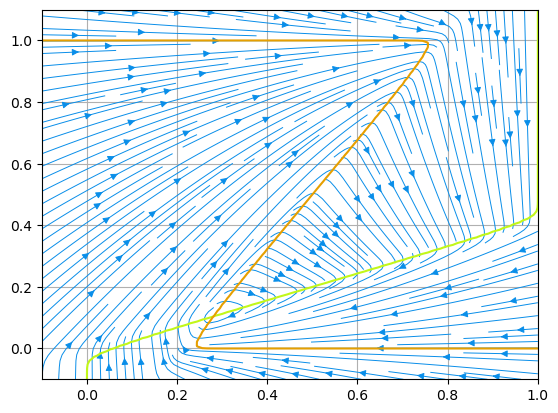
\includegraphics[width=\linewidth]{param graphs/non bistable nullcline plot.png}
        \caption{Sustained oscillations phase plot}
        \label{fig:sustained-oscs-non-bistable-phase-plot}
    \end{subfigure}
    \caption{Phase plots}
    \label{fig:bistable-phase-plots}
\end{figure}

\newpage

\section{Neural field Model}

\begin{flushleft}
    In previous section, when using the Wilson-Cowan system of equations to model mean activity on the population of neurons over time, we made a few assumptions. One major assumption was the lack of spacial dependence to the system. $E(t)$ and $I(t)$ are only dependent on time which is not very representative of the case of neurons in the Neocortex, where we see neurons distributed across space with different regions firing at different times. We can extend the Wilson-Cowan system to a neural field model by adding spacial dependence. By doing this we can see how the activity of excitatory and inhibitory neuron populations interact over time as well as interact with each other in a given space. The extension gives us $E(x,t)$, excitatory activity at position $x$ and $I(x,t)$, inhibitory activity at position $x$.
\end{flushleft}

\begin{flushleft}
    Considering the spatially organised network of neurons, Wilson and Cowen described the connectivity between different regions of the network using functions that depend on the position of the original neuron population on a target population. This yielded,
\end{flushleft}
 
\begin{equation}
    \tau_E\frac{\partial E(x,t)}{\partial t} = -E(x,t) + \phi  \bigg( \int \omega_{EE}(x - x')E(x',t)dx' - \int\omega_{EI}(x-x')I(x',t)dx' +P \bigg)
\end{equation}

\begin{equation}
    \tau_I\frac{\partial I(x,t)}{\partial t} = -I(x,t) + \phi  \bigg( \int \omega_{IE}(x - x')E(x',t)dx' - \int\omega_{II}(x-x')I(x',t)dx' +Q \bigg)
\end{equation}

\begin{flushleft}
    These equations formulated using the Wilson-Cowan to create spacial Wilson-Cowan, where the integrals represent spacial connectivity. 
\end{flushleft}


\subsection{Modelling the neural field}

\begin{flushleft}
We are instructed to consider a two dimensional grid of size N, using vectors $\mathbf{E}(t),\mathbf{I}(t) \in \mathbb{R}^{N}$. Then with this we are able to see the excitatory and inhibitory activity at each grid point. In  the original Wilson-Cowan equations we have coupling coefficients $\omega_{EE},\omega_{EI},\omega_{IE},\omega_{II}$ now as we evolve the model we need to extend these coefficients to matrices. This is because every position on the grid has inhibitory/excitatory value that can also influence other surrounding points. These are defined by 
$W_{EE},W_{EI},W_{IE},W_{II} \ \in \mathbb{R}^{N \times N}$ and are the integrals in the equations above. Thus we can construct simpler equations,
\end{flushleft}

\begin{equation}
    \tau_E\frac{\partial E(x,t)}{\partial t} = -E(x,t) + \phi  \bigg( W_{EE}E(x,t) - W_{EI}I(x,t) + P \bigg)
\end{equation}

\begin{equation}
    \tau_E\frac{\partial I(x,t)}{\partial t} = -I(x,t) + \phi  \bigg( W_{IE}E(x,t) - W_{II}I(x,t) + Q \bigg)
\end{equation}

It is important to note that now our values $P$ and $Q$ have also been converted into $N$ dimensional vectors.

\subsubsection{The connectivity kernel}

We use a Mexican-hat connectivity kernel that implements local excitation with a surrounding inhibitory area (Figure \ref{fig:kernel plots}). It is evaluated on periodic (torus) distances so that coupling is translation-invariant across the grid: neurons in the center and corners behave identically after accounting for periodic boundaries (wrap-around). Therefore, every neuron sees the same neighbourhood and applies the relative distance weightings, removing special edge effects. The variable $\sigma_{\ast\ast}$ defines the interaction length-scale (whether activity is influenced finely/locally or diffusively/globally) and $s_{\ast\ast}$ scales each sub-matrix ($W_{EE}$, $W_{EI}$, $W_{IE}$, and $W_{II}$) to change how strong the influence is.

\begin{figure}[h]
    \centering
    \begin{subfigure}[b]{0.4\textwidth}
        \centering
        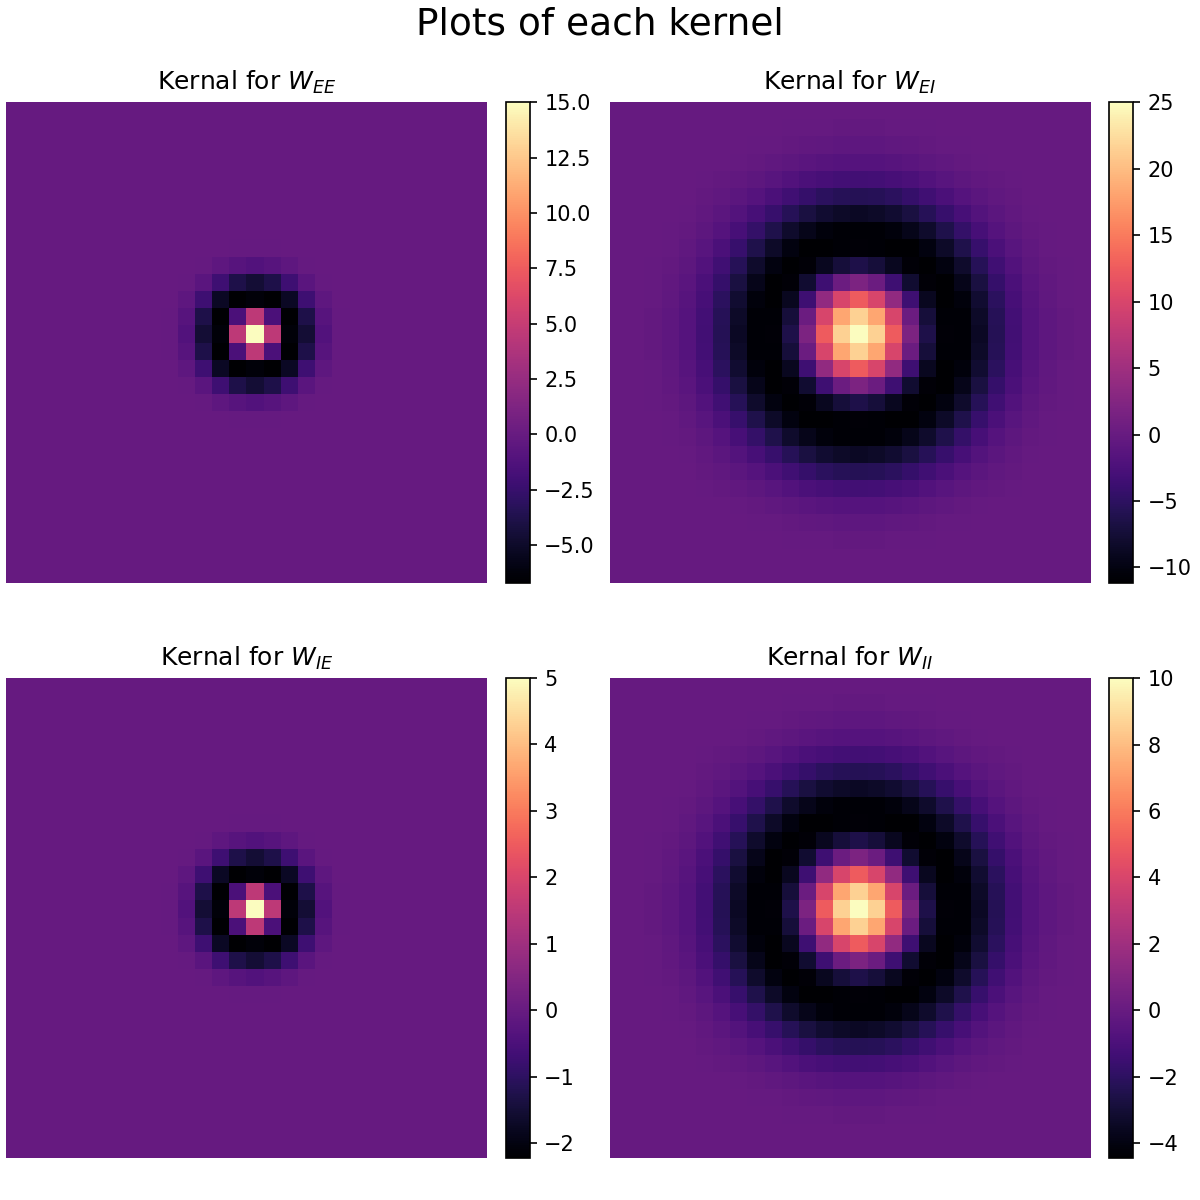
\includegraphics[width=\linewidth]{kernels/kernel_plot.png}
        \caption{Plots of each kernel in the grid space where colour represents the strength of local connectivity around a point.}
        \label{fig:kernel plot}
    \end{subfigure}
    \qquad \quad
    \begin{subfigure}[b]{0.4\textwidth}
        \centering
        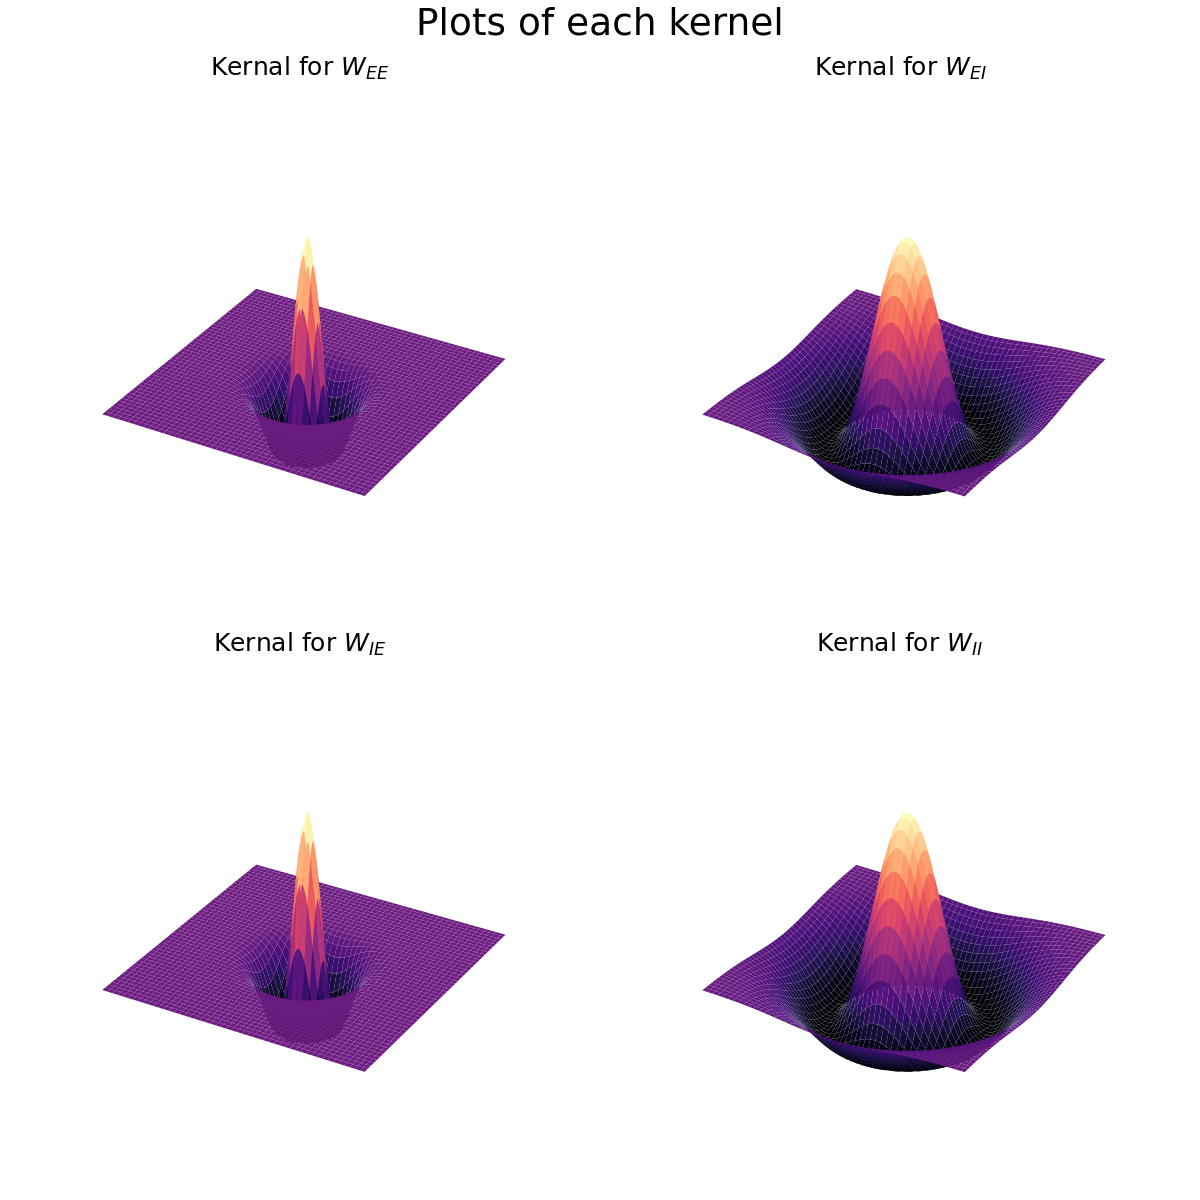
\includegraphics[width=\linewidth]{kernels/kernel_plot_3d.png}
        \caption{Plots of each kernel in 3D space where z-axis represents the strength of local connectivity around a point.}
        \label{fig:kernel plot 3d}
    \end{subfigure}
    \caption{Plots of each kernel using the different $\sigma$ values ($\sigma_{EE}$, $\sigma_{EI}$, $\sigma_{IE}$, and $\sigma_{II}$).}
    \label{fig:kernel plots}
\end{figure}

\newpage

\subsubsection{W sub-matrices}

The $W$ sub-matrices are created during the initialisation of the neural field. They only need to be generated once as they describe the connectivity between each neuron in the field, and this never changes during run time.

One sub-matrix (kernel) is generated per connection type ($E \rightarrow E$, $E \rightarrow I$, $I \rightarrow E$, and $I \rightarrow I$): first, by computing the distance between every pair of grid points (using periodic wrap-around); then, applying a Gaussian kernel to convert distance into a Gaussian fall-off - connectivity decaying smoothly with distance; converting the Gaussian into a Mexican-hat shape - local excitation with surrounding inhibition; finally, scaling the kernel by a corresponding strength $s_{\ast\ast}$.

\begin{lstlisting}[language = python,label={searchsetup}, mathescape=false, breaklines=true]
    self.W = {
        "EE": self.gaussian_weight_matrix(self.sigma_EE, self.strength_EE),
        "EI": self.gaussian_weight_matrix(self.sigma_EI, self.strength_EI),
        "IE": self.gaussian_weight_matrix(self.sigma_IE, self.strength_IE),
        "II": self.gaussian_weight_matrix(self.sigma_II, self.strength_II),
    }

    def gaussian_kernel(x, sigma):
        return np.exp(-x / (2.0 * (sigma ** 2))).astype(np.float32)

    def get_pairwise_periodic_distance_squared(self, x, y):
        dx = np.abs(x.reshape(self.N, 1) - x.reshape(1, self.N))
        dy = np.abs(y.reshape(self.N, 1) - y.reshape(1, self.N))
        if self.periodic:  # If it is periodic we need to wrap around.
            dx = np.minimum(dx, self.grid_size[0] - dx).astype(np.float32)
            dy = np.minimum(dy, self.grid_size[1] - dy).astype(np.float32)
        return dx ** 2 + dy ** 2

    def kernel_weight_matrix(self, sigma, strength):
        distances_squared = self.get_pairwise_periodic_distance_squared(*self.grid_coordinates)
        gaussian = self.gaussian_kernel(distances_squared, sigma)
        mexican_hat = (1 - distances_squared / (sigma ** 2)) * gaussian
        return (mexican_hat * strength).astype(np.float32)
\end{lstlisting}

\section{Numerically solving the Neural Field model}

\begin{flushleft}
    In the last section we extended the Wilson-Cowan equations to a neural field model by including spatio-temporal behaviour. We can now numerically solve this for a range of parameters and initial conditions.
\end{flushleft}

\begin{flushleft}
    Previously, in section 2 we numerically solved the Wilson-Cowan equations and found 3 common behaviours: bifurcations, decaying oscillatory behaviour, and sustained oscillations. We can use these values in the extended Wilson-Cowan system to look at not only how the behaviour changes over time (or time step $t$) but in a spatio-temporal view. In the plotting we are using the variable $\sigma$ to represent the local connectivity between neurons and are plotting the activity of excitatory and inhibitory neurons over time.
\end{flushleft}

\subsection{Bifurcations}

\begin{flushleft}
    To begin, we took the parameter values and initial conditions from Table \ref{bif}, these being the parameter values and initial conditions to achieve stable points in the model. When using these in the neural field model coded in section 4 with our given strength parameters and mapping the excitatory/inhibitory activity over time.
\end{flushleft}

\begin{figure}[!h]
    \centering
    \begin{subfigure}[b]{0.35\textwidth}
        \centering
        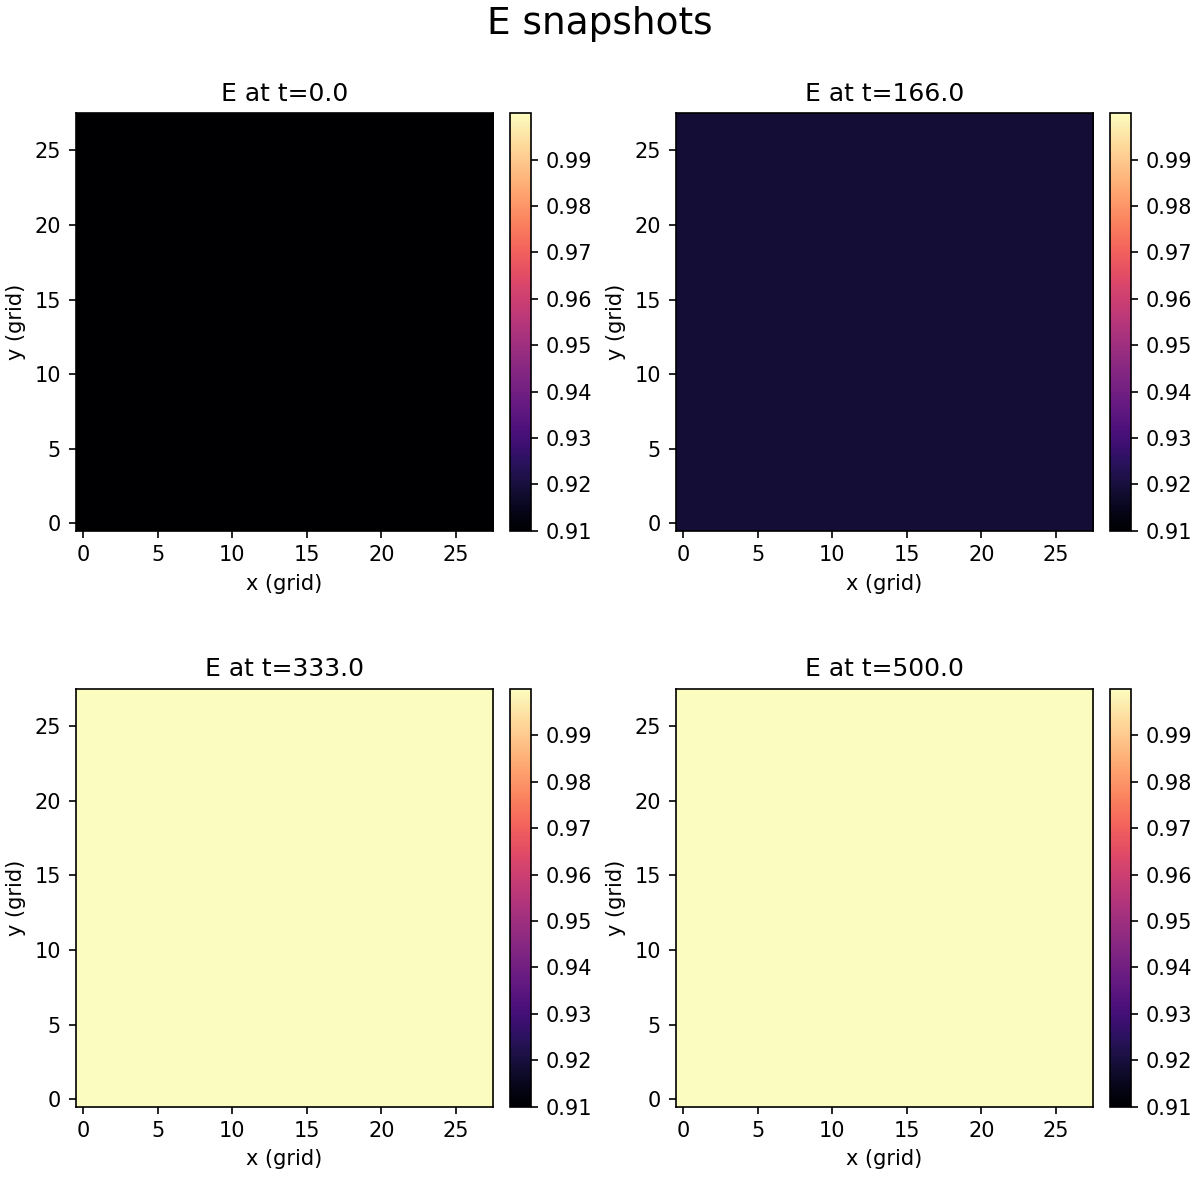
\includegraphics[width=\textwidth]{Heatmaps/E_snapshots_bif.png}
        \label{fig:Heatmaps of E bif}
    \end{subfigure}
    \qquad \quad
    \begin{subfigure}[b]{0.35\textwidth}
        \centering
        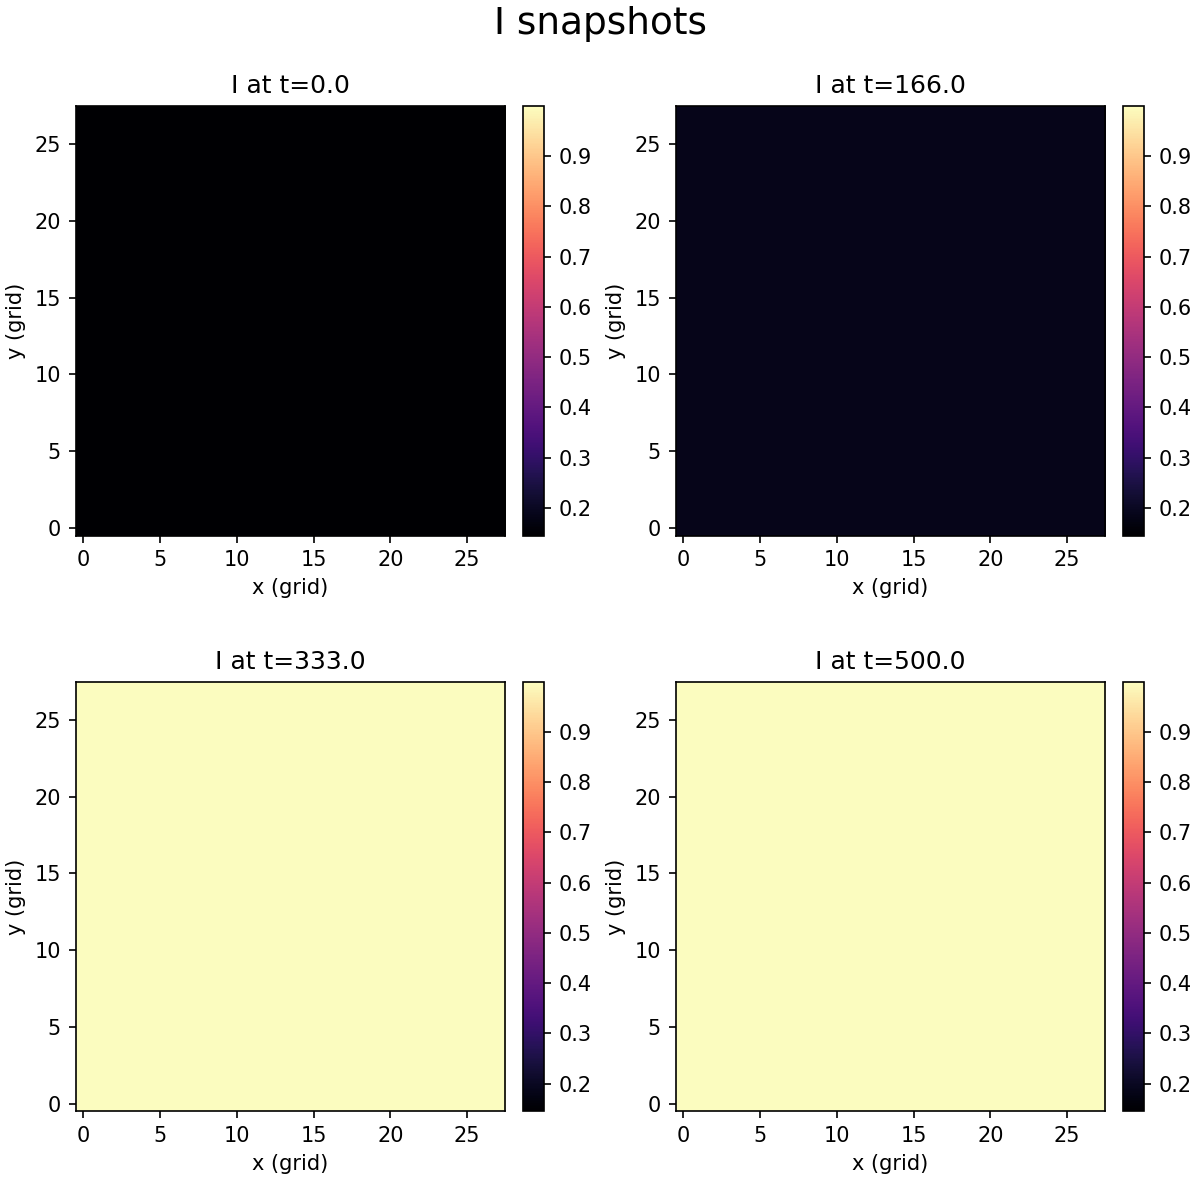
\includegraphics[width=\textwidth]{Heatmaps/I_snapshots_bif.png}
        \label{fig: Heatmaps of I bif}
    \end{subfigure}
    \caption{Snapshots of the Inhibitory/Excitatory activity spatio-temporally - from Bifurcation behaviour parameters}
    \label{fig:heatmaps bif}
\end{figure}


\begin{flushleft}
    In both the excitatory and inhibitory snapshots in Figure \ref{fig:heatmaps bif} we can see that, at each time step, the activity across the grid is uniform showing us that the activity is at a steady state. This exactly reflects the neuron activity in Figure \ref{fig:stable only}, where you can see the excitatory activity increases up to approximately $1$ from $0.9$ and the inhibitory activity increases from $0.1$ to around $0.5$.
\end{flushleft}


\begin{minipage}[t]{0.39\textwidth}
    \centering
    \vspace{0pt}
    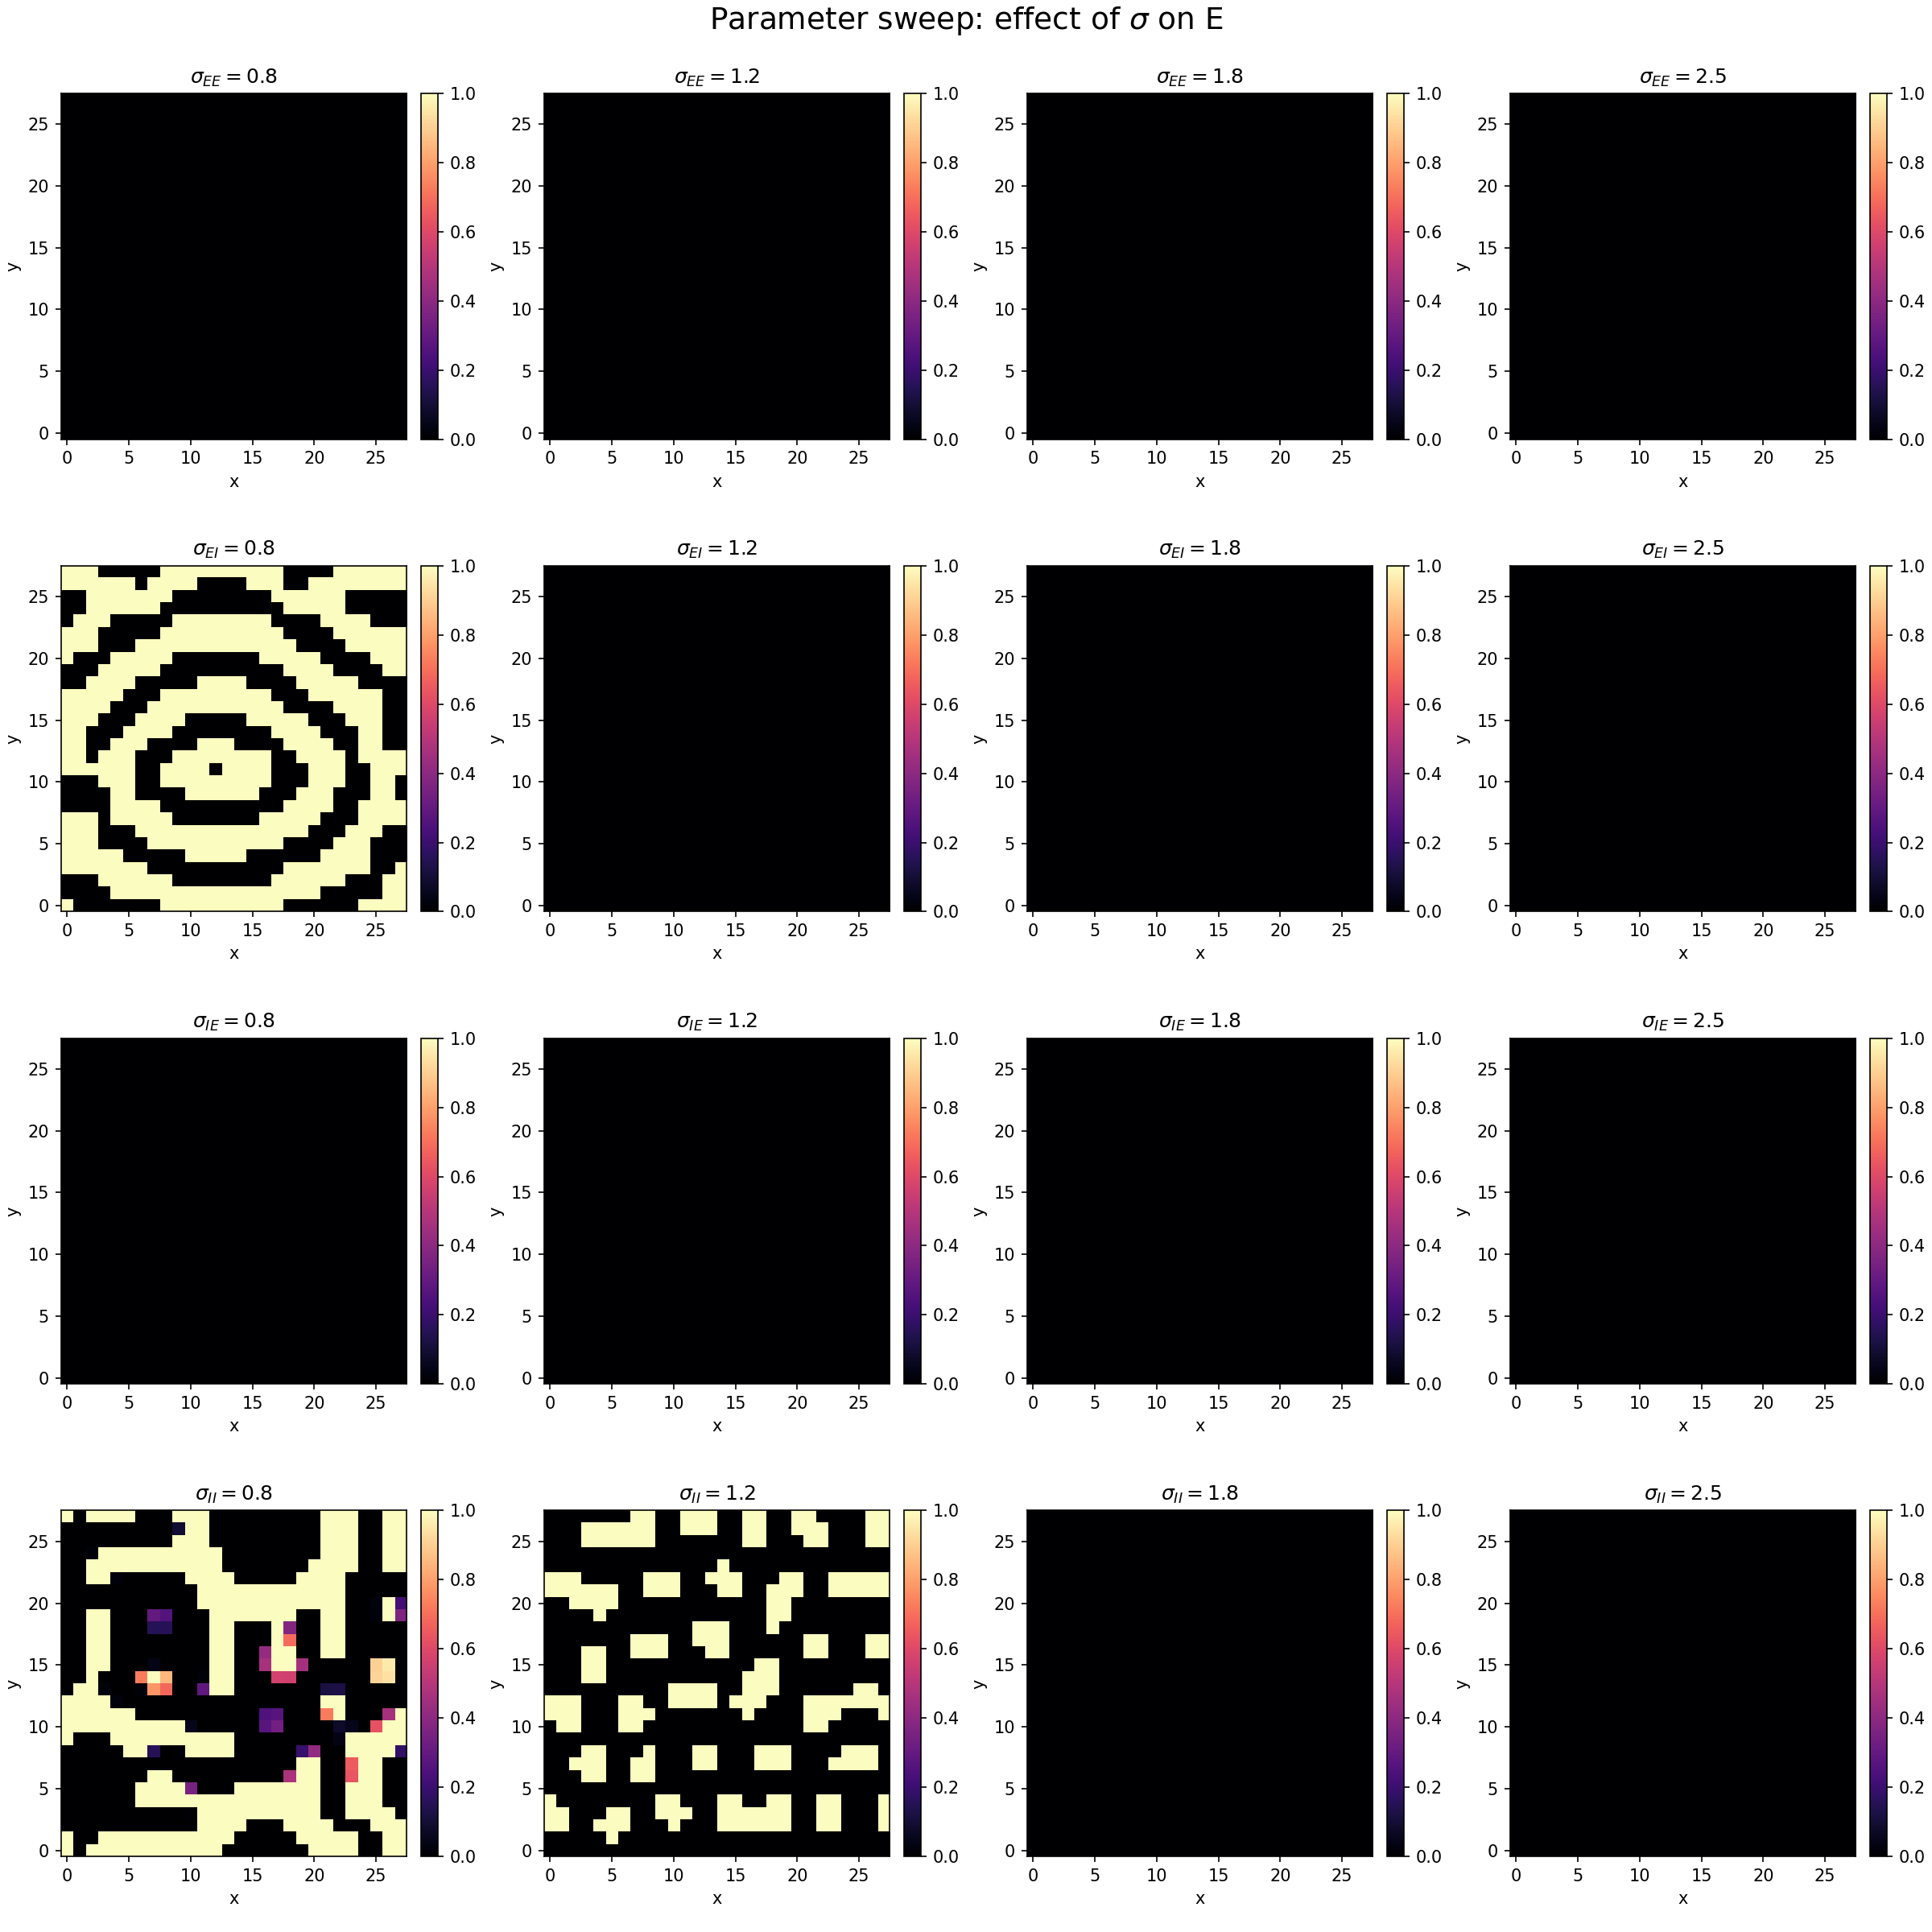
\includegraphics[width=0.8\linewidth]{Heatmaps/parameter_sweep_sigma_E_bif.png}
    \label{fig:parameter_sweep_sigma_E_bif.png}
    \captionof{figure}{Parameter sweeps for different values for each weighting coefficient and its effect on excitatory activity spacially - from bifurcation behaviour  parameters }
\end{minipage}
\hfill
\begin{minipage}[t]{0.59\textwidth}
    \vspace{0pt}
\centering
    \textbf{Parameter Sweep}
    
\begin{flushleft}
Now using the majority of the same parameters, we can investigate the different weighing coefficients on the neural field model using a parameter sweep (Figure \ref{fig:parameter_sweep_sigma_E_bif.png}), focusing on the excitatory population. Using the bifurcation (stable-point) parameters, we find that there is a limited number of plots that exhibit patterns. This is because, for most settings, the field remains linearly stable and therefore stays uniform.

The only plots that show patterns are those with $\sigma_{EI}=0.8$ and $\sigma_{II} \in \{0.8, 1.2\}$, this is because these particular inhibitory connectivities are small enough to avoid the global stabilising effect on inhibition, becoming locally unstable.
\end{flushleft}

\end{minipage}

\subsection{Decaying Oscillation}

\begin{flushleft}
Now taking the parameter values and initial conditions from Table \ref{Dam} and using these in the neural field model. When mapping the excitatory/inhibitory activity across the grid over time.
\end{flushleft}

\begin{figure}[!h]
    \centering
    \begin{subfigure}[b]{0.35\textwidth}
        \centering
        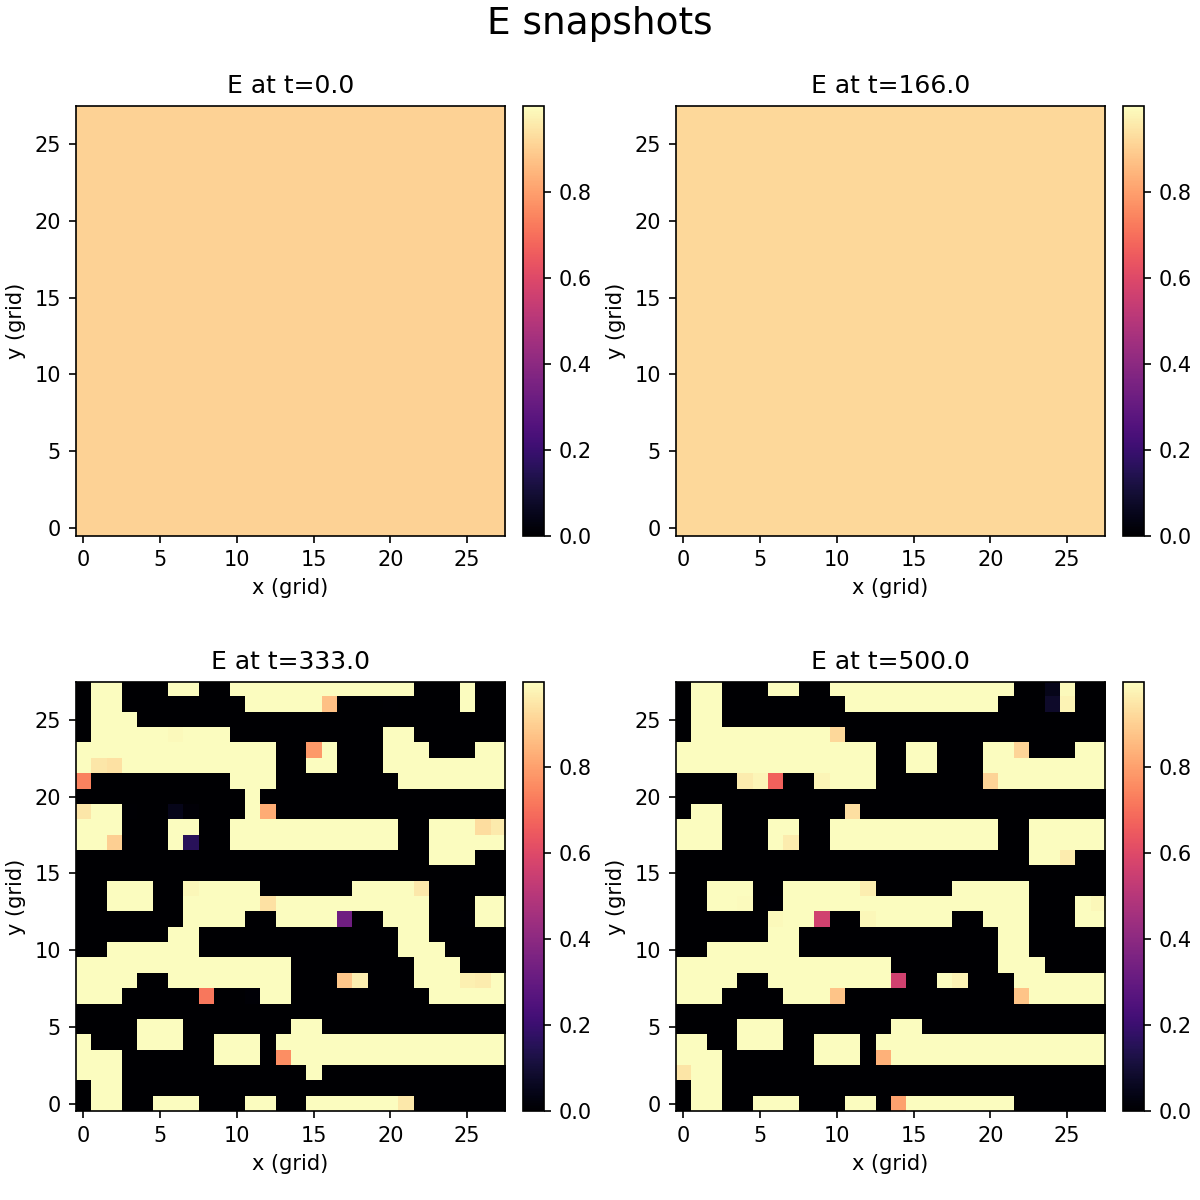
\includegraphics[width=\textwidth]{Heatmaps/E_snapshots_damped.png}
        \label{fig:heatmaps of E damped}        
    \end{subfigure}
    \qquad \quad
    \begin{subfigure}[b]{0.35\textwidth}
        \centering
        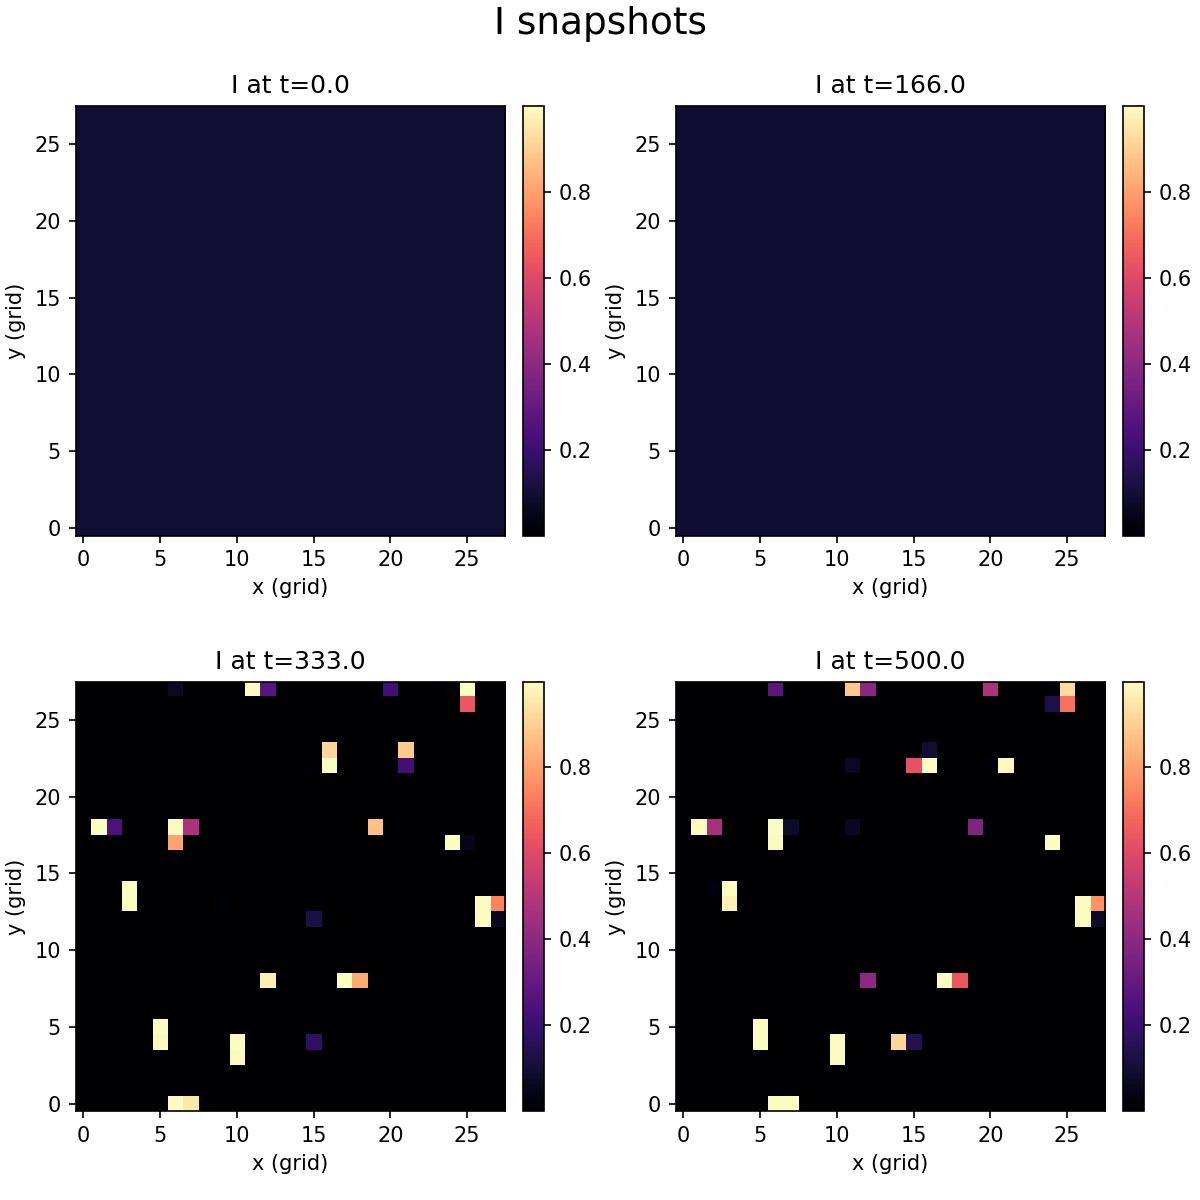
\includegraphics[width=\textwidth]{Heatmaps/I_snapshots_damped.png}
        \label{fig:heatmaps of I damped}        
    \end{subfigure}
    \caption{Snapshots of the Inhibitory/Excitatory activity spatio-temporally - from decaying oscillatory behaviour parameters}
    \label{fig:heatmaps damped}
\end{figure}


\begin{flushleft}
    In the excitation snapshots (Figure \ref{fig:heatmaps of E damped}) we can see it is uniform across the grid at $t=0$ and $t=166$. Then, we can see regions of excitation start to appear. Using these parameters, the pattern of the grid seems to be showing labyrinth-like patterns of high excitation activity. Finally, we see that areas of previously lower excitation have increased. This pattern is non uniform, but a stable system with areas of high excitatory action.
    
    In the inhibitory snapshots (Figure \ref{fig:heatmaps of I damped}) we can see the same uniform and steady state of inhibition over the grid in the first time steps. Then at $t=333$ and onwards, we can see that there are small areas of inhibitory activity, this is to respond to the regions of high excitation and provide local negative feedback aiming to return the system to a steady state.
\end{flushleft}

\begin{minipage}[t]{0.39\textwidth}
    \centering
    \vspace{0pt}
    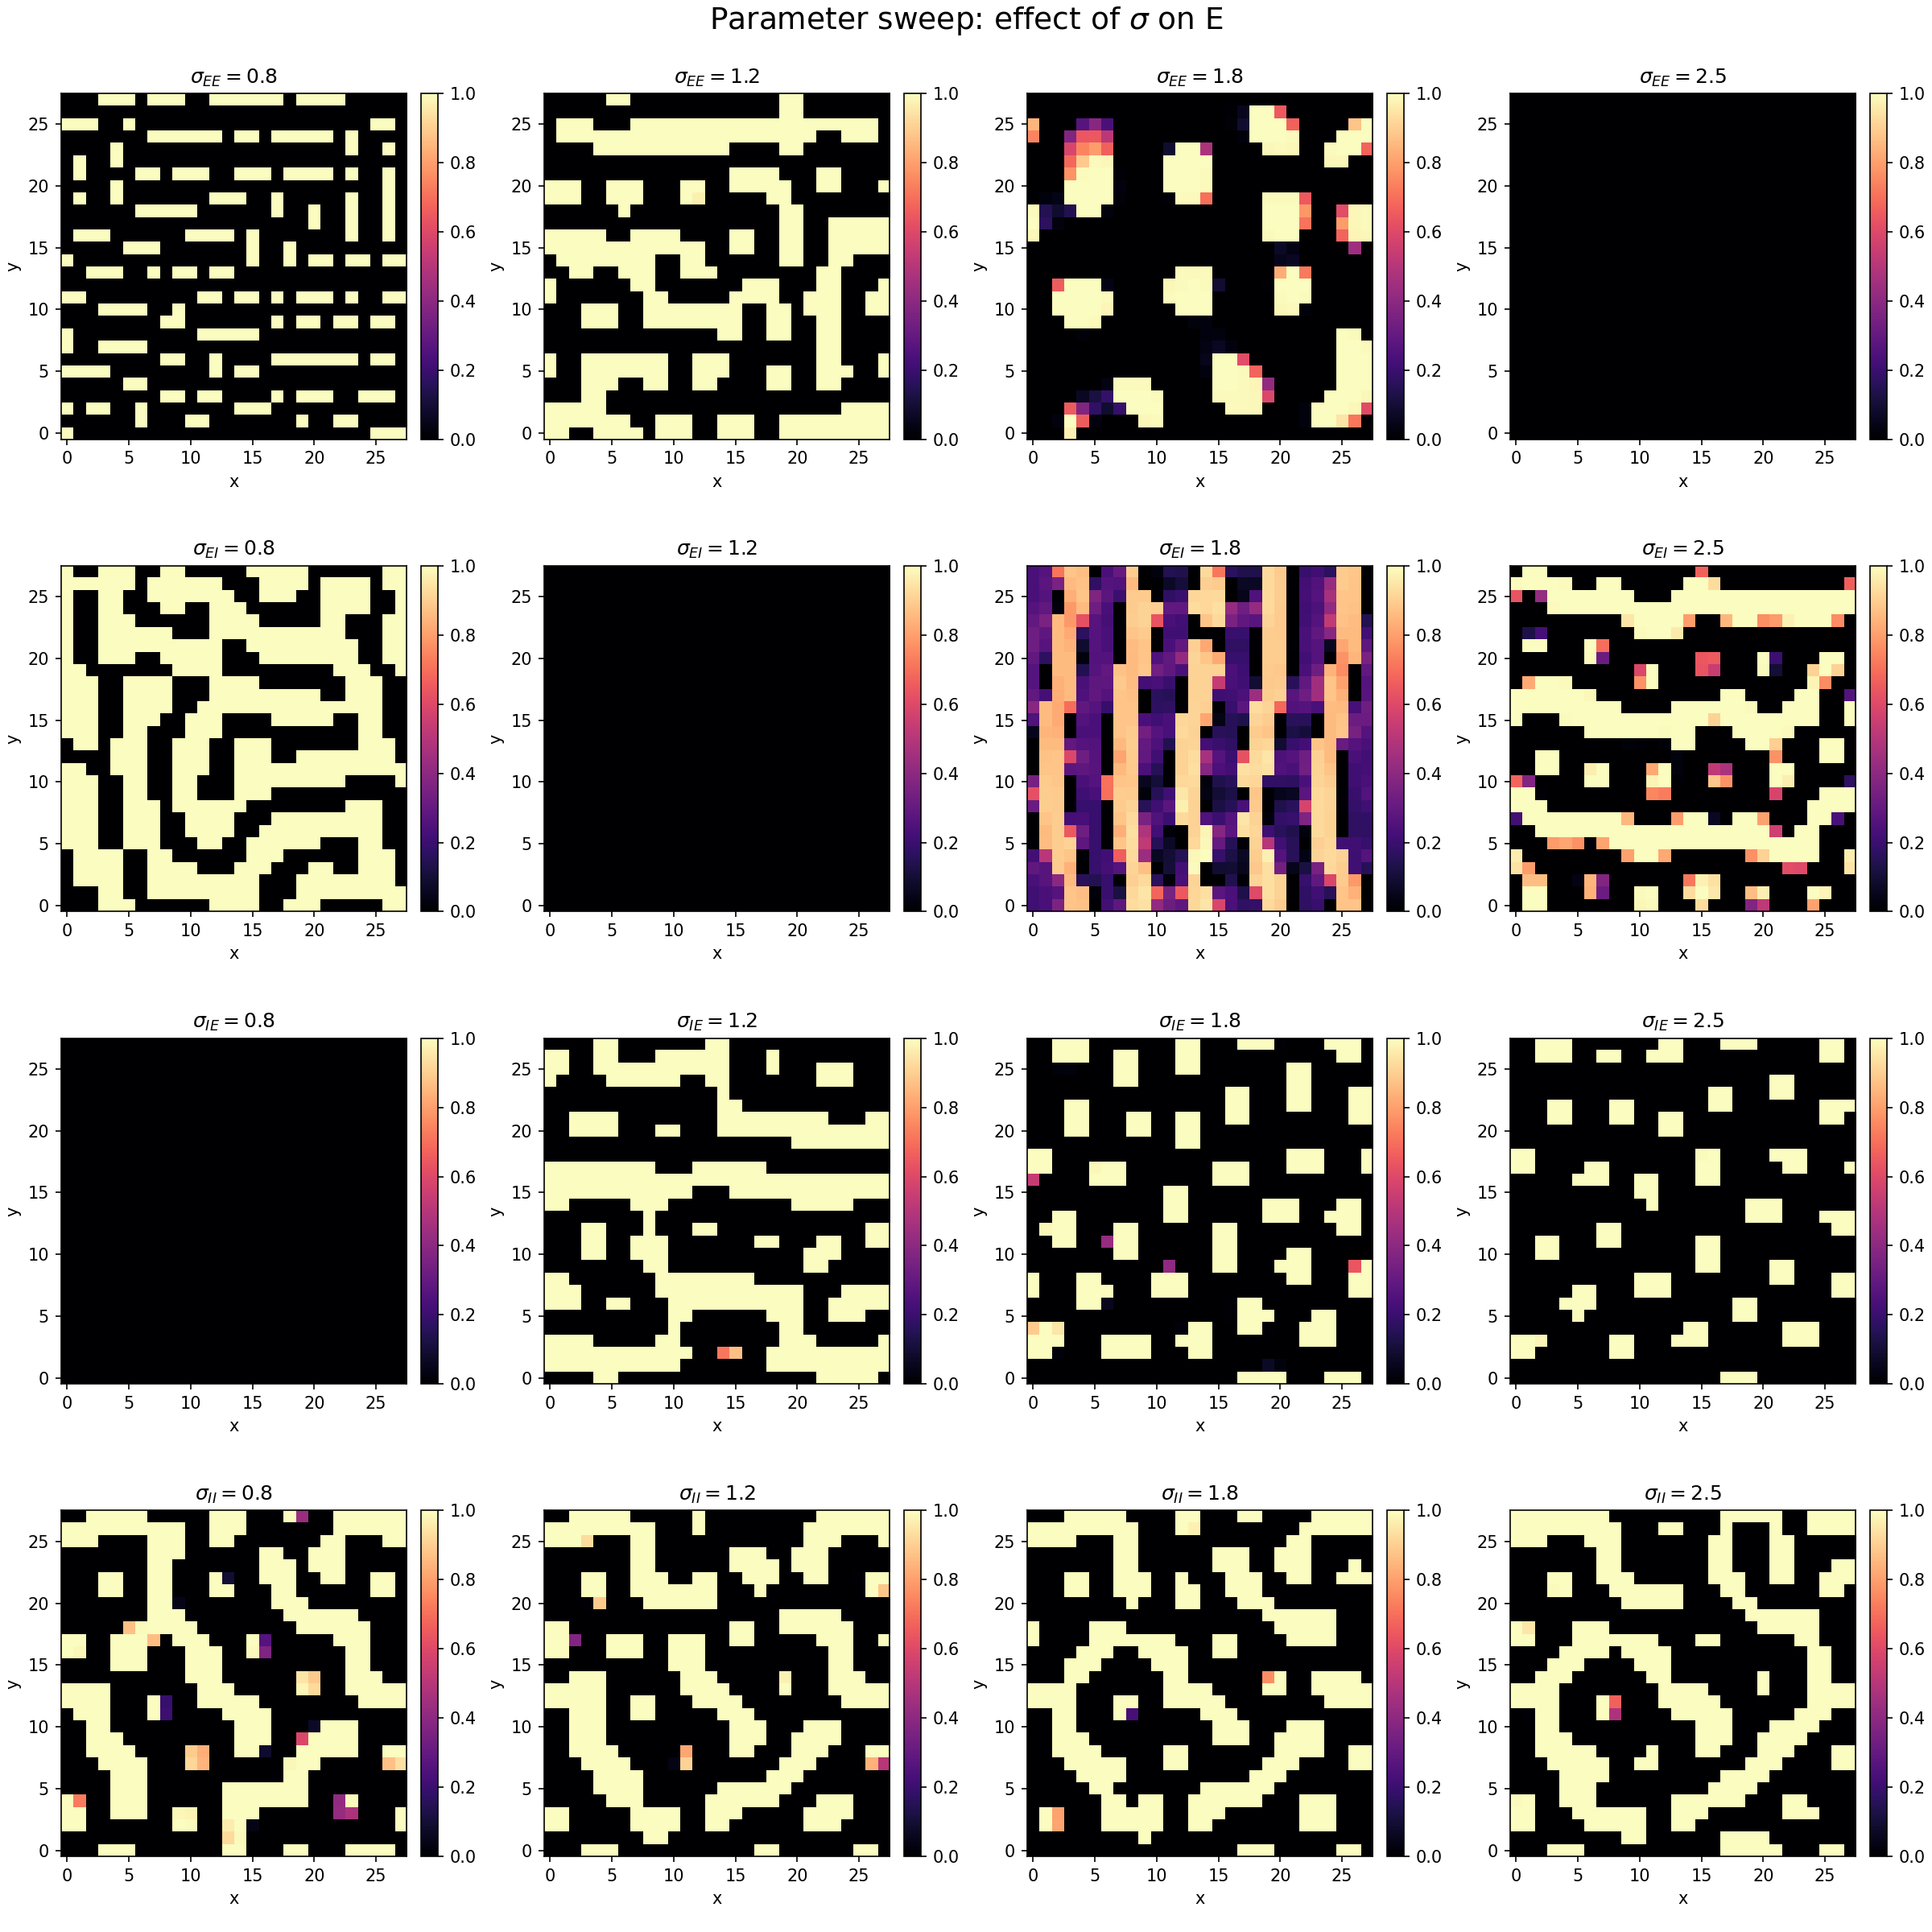
\includegraphics[width=0.8\linewidth]{Heatmaps/parameter_sweep_sigma_E_damped.png}
    \label{fig:parameter_sweep_sigma_E_damped}
    \captionof{figure}{Parameter sweeps for different values for each weighting coefficient and its effect on excitatory activity spatially - from decaying oscillatory behaviour  parameters}
\end{minipage}
\hfill
\begin{minipage}[t]{0.59\textwidth}
        \vspace{0pt}
    \centering
        \textbf{Parameter Sweep}
    
    \begin{flushleft}
            In Figure \ref{fig:parameter_sweep_sigma_E_damped}, we sweep across the same $\sigma$ parameters as before:
            \begin{itemize}
                \item $\sigma_{EE}$: With $\sigma_{EE}=0.8$ the field creates dense labyrinths - interlocking walls separated by dark corridors. As $\sigma_{EE}$ increases, these channels thicken and produce meanders. At $\sigma_{EE}=1.8$, these channels break into islands of high activation. Finally, the grid becomes uniform.
                \item $\sigma_{EI}$: $\sigma_{EI}=0.8$ still allows for labyrinth patterns to form. Then, $\sigma_{EI}=1.2$ is entirely dark, showing strong suppression on E. $\sigma_{EI}=1.8$ shows a vertical striped pattern and broader inhibition ($\sigma_{EI}=2.5$) shows a softened pattern of horizontal stripes. This row illustrates how changing $\sigma_{EI}$ varies the spatial mode (extinguished, stripes, and labyrinths).
                \item $\sigma_{IE}$: An initially uniform grid (with $\sigma_{IE}=0.8$) becomes labyrinth-like with ring-like pockets and then granulates into an array of compact spots as $\sigma_{IE}$ continues to increase.
                \item $\sigma_{II}$: Looped labyrinths form immediately and partially dissolve into open ring-like pockets as $\sigma_{II}$ increases.
            \end{itemize}
    \end{flushleft}

\end{minipage}



\subsection{Sustained Oscillations: Limit cycles}

\begin{flushleft}
Finally taking the parameter values and initial conditions from Table \ref{Osc}, when using these in the neural field model and mapping the excitatory/inhibitory activity across the grid over time.
\end{flushleft}

\begin{figure}[!h]
    \centering
    \begin{subfigure}[b]{0.35\textwidth}
        \centering
        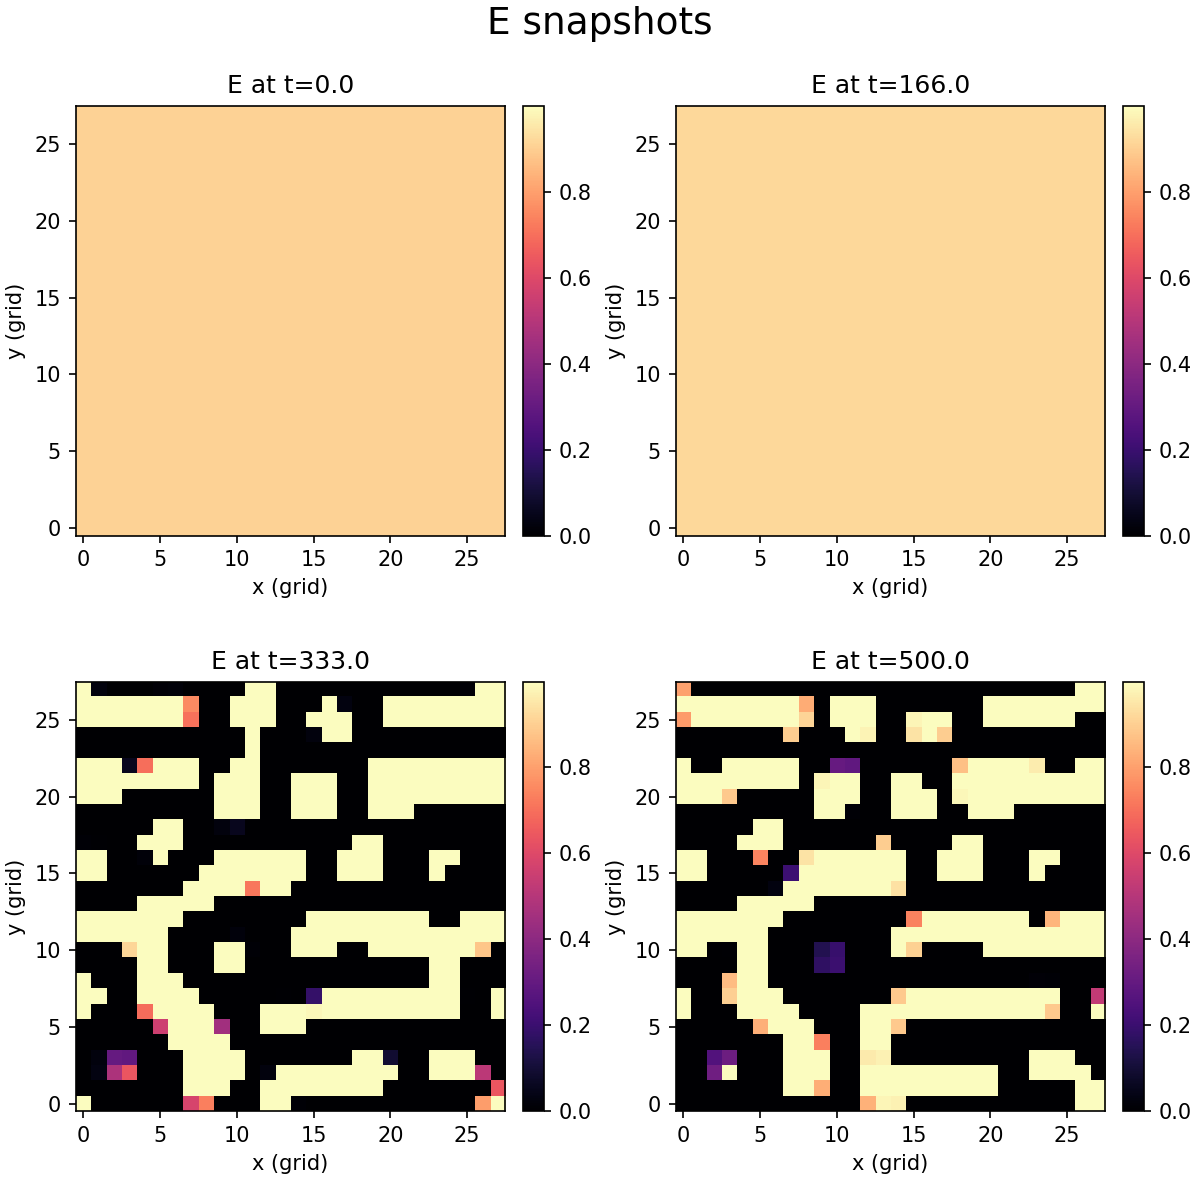
\includegraphics[width=\textwidth]{Heatmaps/E_snapshots_osc.png}
        \label{fig:heatmaps of E limit}        
    \end{subfigure}
    \qquad \quad
    \begin{subfigure}[b]{0.35\textwidth}
        \centering
        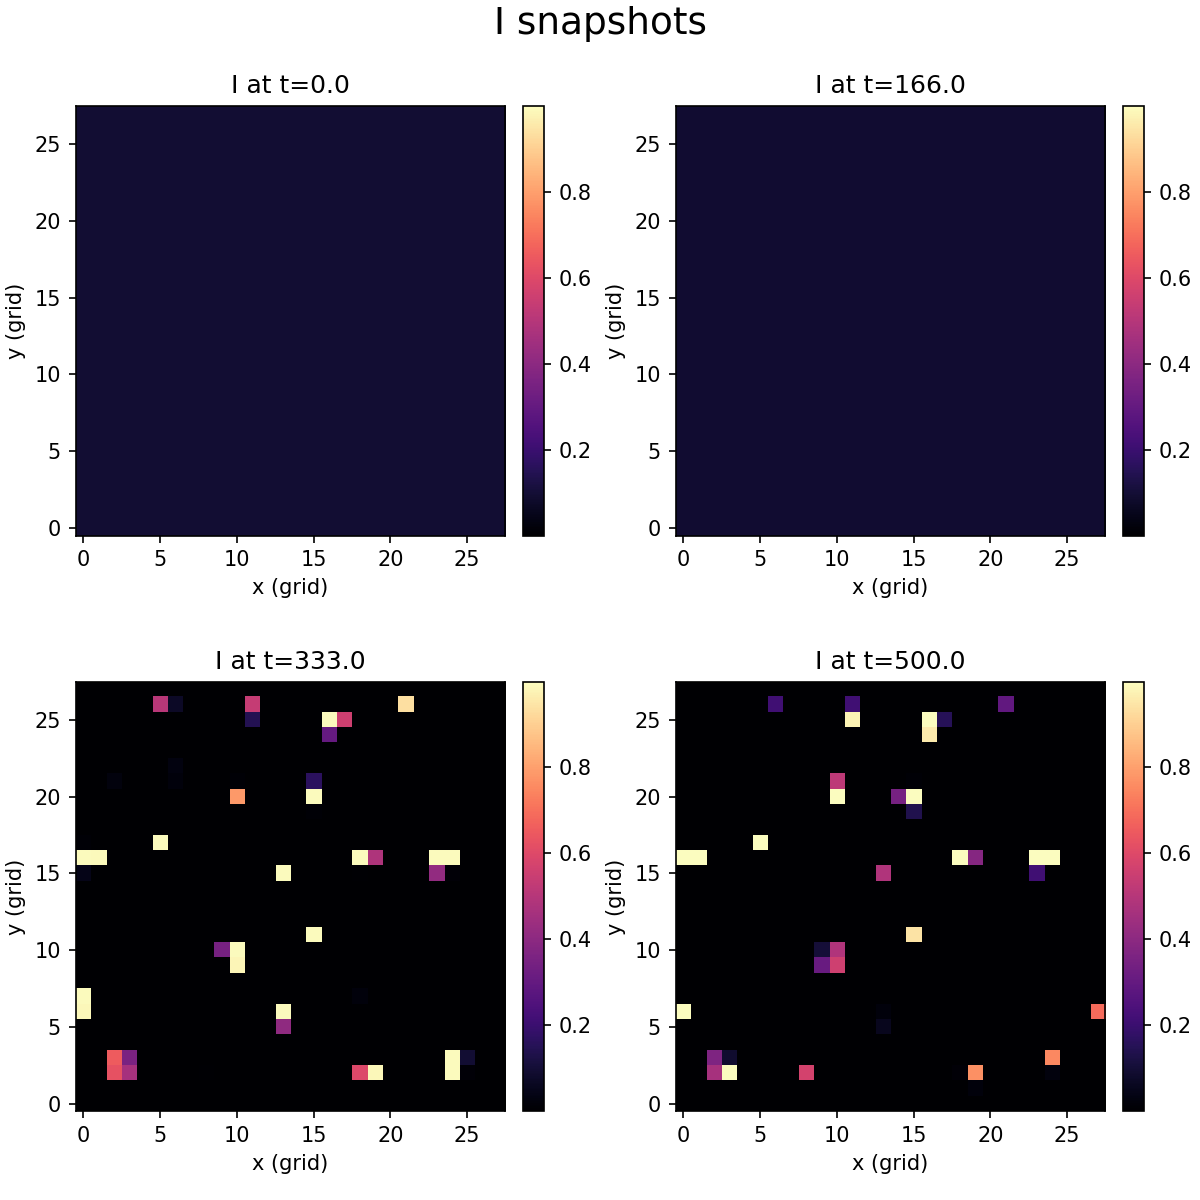
\includegraphics[width=\textwidth]{Heatmaps/I_snapshots_osc.png}
        \label{fig:heatmaps of I limit}        
    \end{subfigure}
    \caption{Snapshots of the Inhibitory/Excitatory activity spatio-temporally - from Limit cycle behaviour parameters}
    \label{fig:heatmaps limit}
\end{figure}


\begin{flushleft}
    In the excitatory snapshots (Figure \ref{fig:heatmaps of E limit}) across the grid we can see uniform activity across the excitatory population in space during our first time steps. Then in the next two plots we can see meander-like patterns appear with regions of high excitatory activity. We see clear boundaries between active and inactive regions. 
    
    In the inhibitory snapshots (Figure \ref{fig:heatmaps of I limit}) we can see a similar pattern to our damped plots with areas of inhibition. This is to respond to the regions of high excitation and provide local negative feedback aiming to return the system to a steady state.
\end{flushleft}
    
\begin{flushleft}
    \begin{center}
    \textbf{Parameter Sweep}
    \end{center}

    The parameter sweep (Figure \ref{fig:parameter sweep osc}) for the limit cycle looks almost identical to our damped oscillations, this is because the spatial mode of our Mexican-hat connectivity hasn't changed as this is independent of steady or oscillatory activity. However, the brightness of the points would oscillate over time. It is also important to note that the activity of E and I will oscillate out of phase with each other, as seen in Figure \ref{fig:timeseries osc} where inhibitory neuron activity is a reflection of excitatory activity.
\end{flushleft}

\begin{figure}[!h]
    \centering
    \begin{subfigure}[b]{0.35\textwidth}
        \centering
        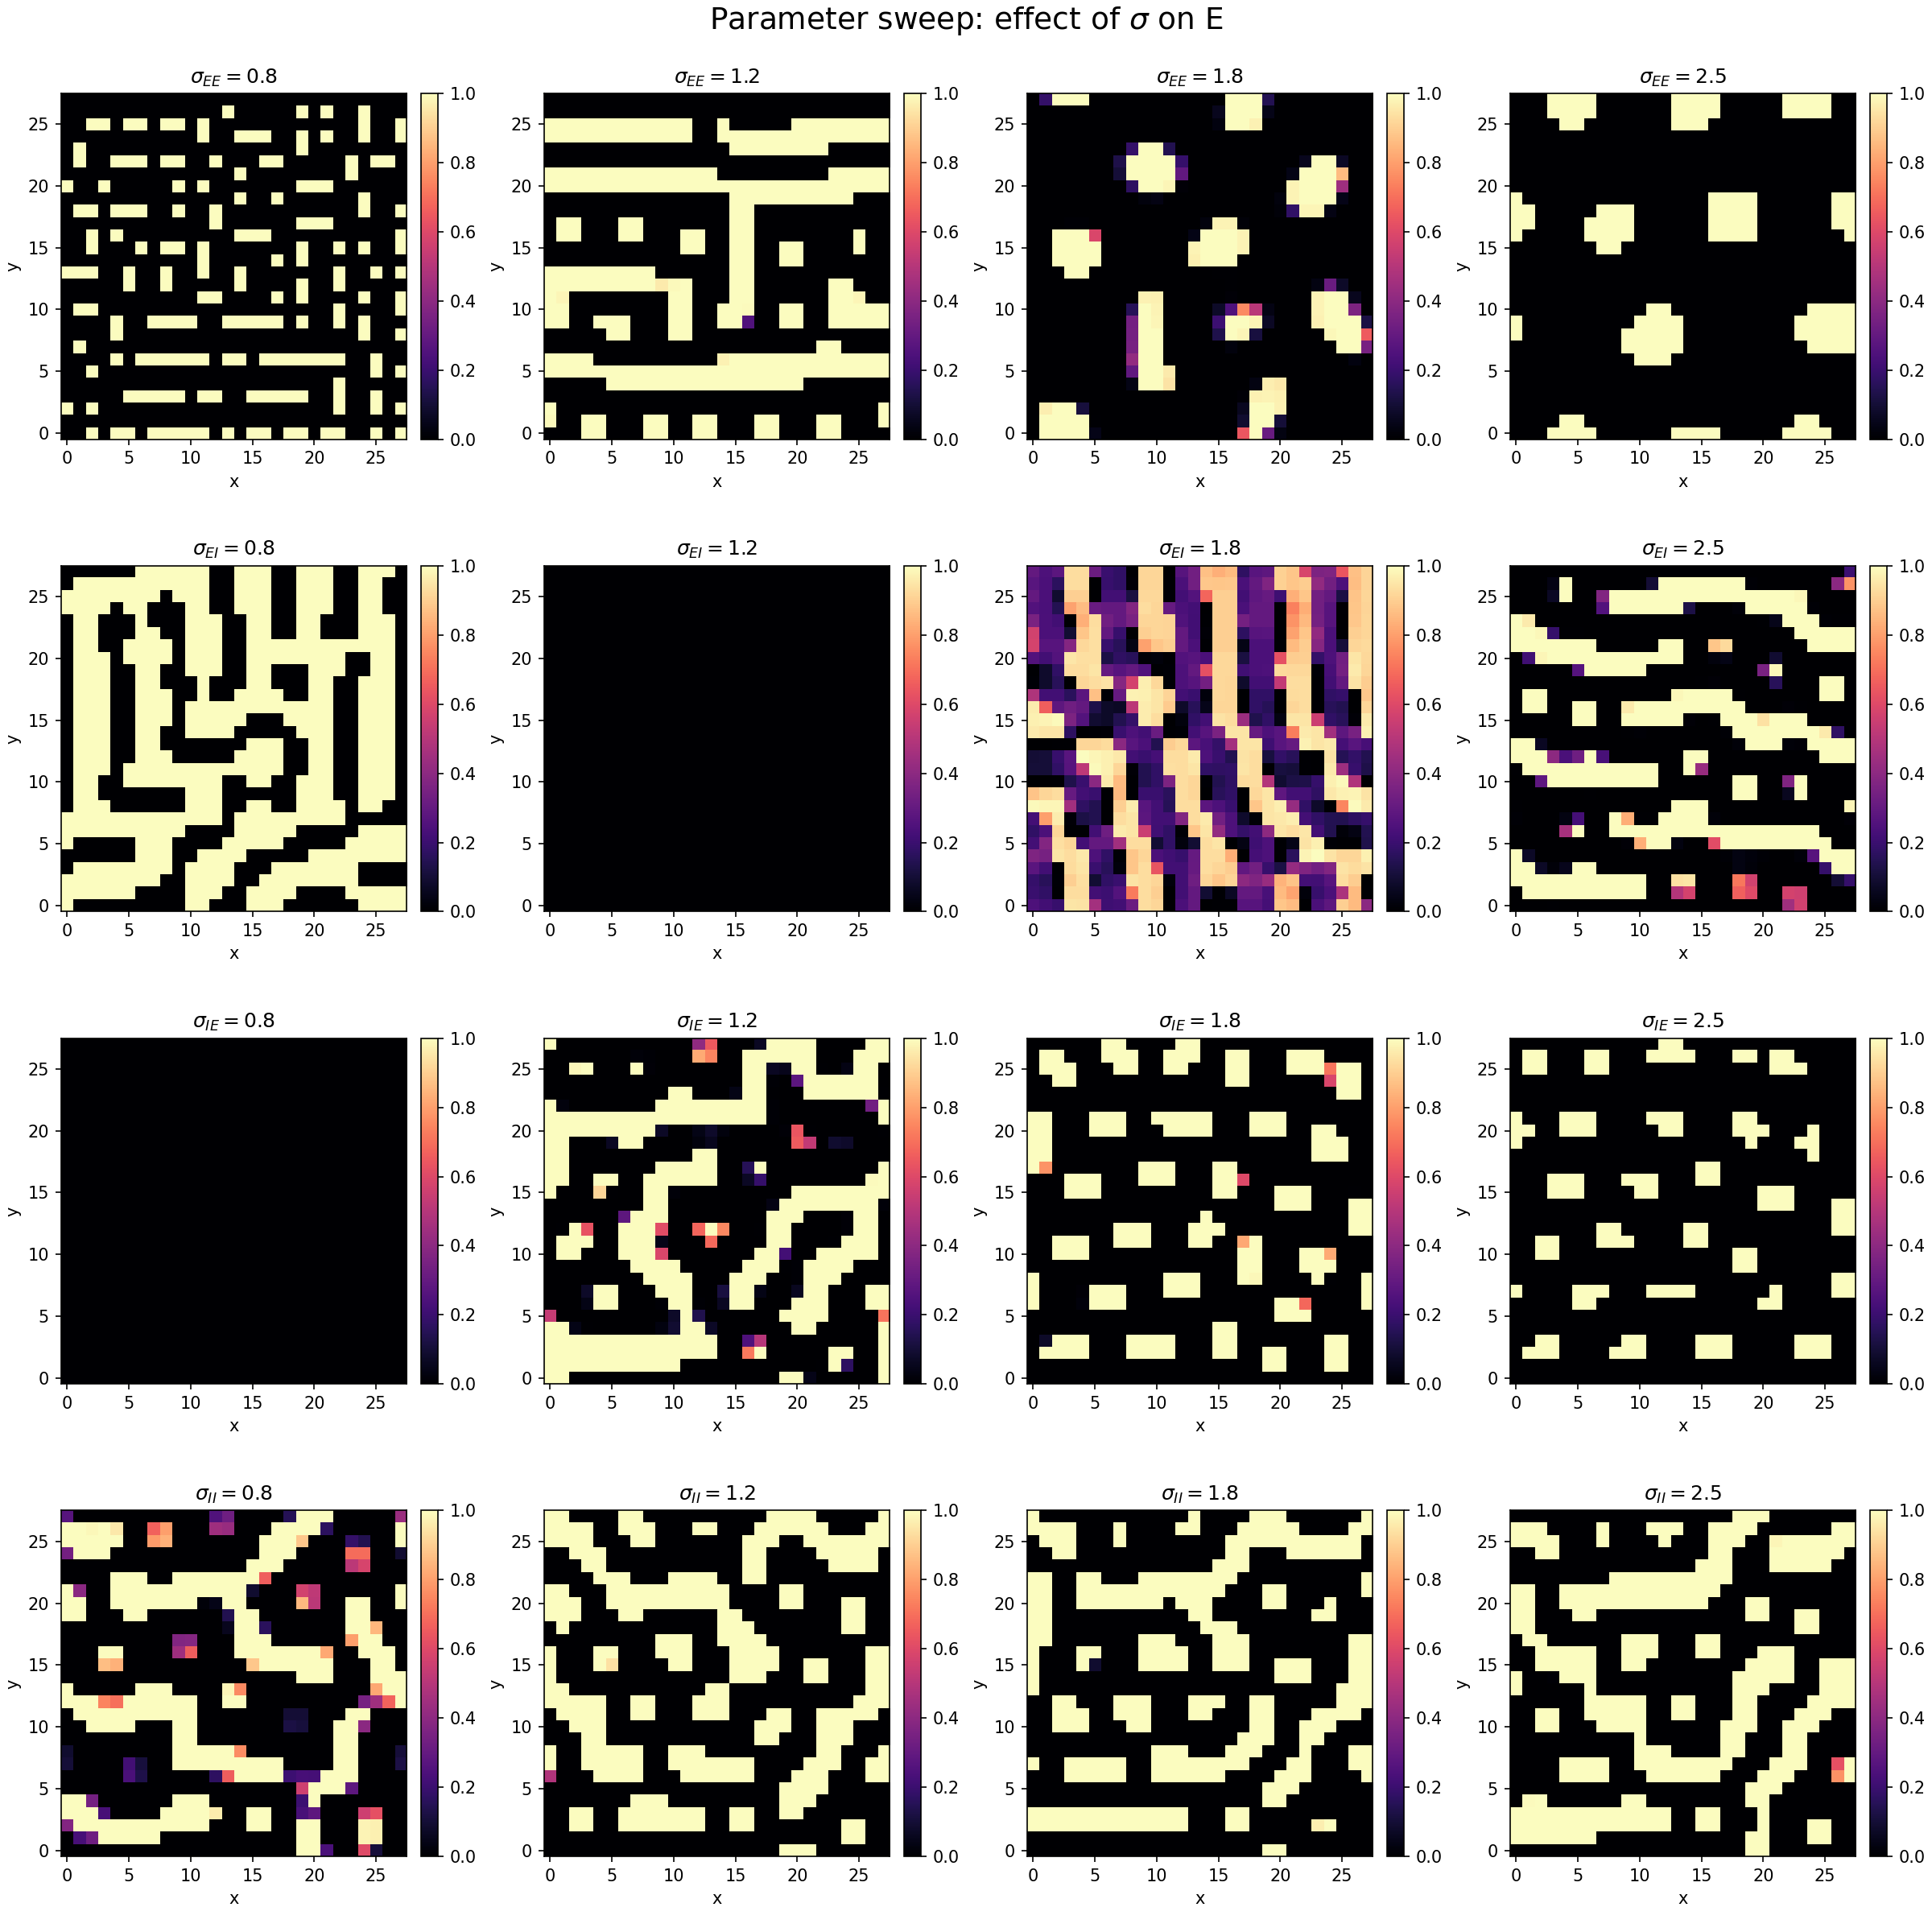
\includegraphics[width=\linewidth]{Heatmaps/parameter_sweep_sigma_E_osc.png}
        \caption{Parameter sweeps for different values for each weighting coefficient and its effect on excitatory activity spatially - from limit cycle behaviour  parameters}
        \label{fig:parameter sweep osc}
    \end{subfigure}
    \qquad \quad
    \begin{subfigure}[b]{0.35\textwidth}
        \centering
        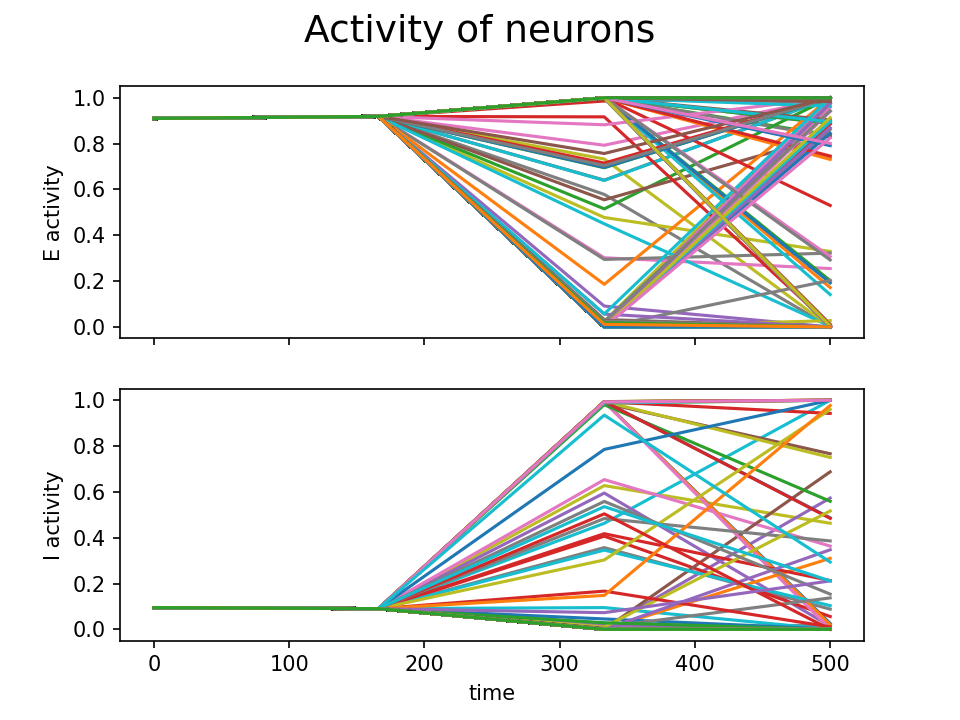
\includegraphics[width=1.2\linewidth]{Heatmaps/timeseries_osc.png}    
        \caption{Time series of limit cycle neurons, showing out of phase timing (colours may differ but shape is the same).}
        \label{fig:timeseries osc}
    \end{subfigure}
    \caption{Parameter sweep and time series of limit cycle conditions.}
    \label{fig:parameter sweep and timeseries osc}
\end{figure}

\section{Combining Wilson-Cowan and Machine learning}

    Now that we have developed a 2-dimensional neural field in section 4 and explored what changes to parameters do to the outcome of the simulation in section 5,
    we can ask whether we could adapt this to be used alongside machine learning.
    We will now investigate if the MNIST dataset (a dataset of hand-drawn digits $0-9$) can be applied to the neural field model and what processes can be carried out
    in order to achieve this.

    \subsection{Accessing and using the MNIST dataset}

    Until coming across \texttt{kagglehub} and the resource \texttt{hojjatk/mnist-dataset} \cite{mnist-dataset}, finding the dataset was initially quite difficult or rather involved,
    but this python package allowed us to download the dataset directly onto the computer and access it via \texttt{numpy}.
    This then provided the training and test datasets.
    
    Now, the images could be passed into the original \texttt{WCNeuralField} as \texttt{P} when resized from 2 dimensions into
    a single dimensional array of size $N^{2}$ ($N$ being grid size from earlier) and then simulated between time step 0 and some
    defined time \texttt{total\_time}.

    \subsection{Analysis of features}

    In order to make sense of the data being processed here, we need to convert it from (effectively) an NxN array into
    a feature vector we can place in some space and compare with other feature vectors.
    There are a variety of methods that could be used to convert this information into feature vectors in order to identify
    particular outputs from our neural field with their number counterparts:

    \begin{itemize}
        \item \textbf{k-th nearest neighbours:}
        We would use this to find $k$ neighbours to our point in space, and then find the mode average of the digit associated
        with these neighbours to give us the most common digit in that area of space.
        
        This seems ideal, as it would act as an averager for all the points associated with a certain
        digit.
        However, since we are dealing with such large dimensions ($28\times28=784$ dimensions),
        this method begins to break down quickly:

        \begin{itemize}
            \item Distance metrics become meaningless at this scale and, as a result, all points start to appear equally far
            from one another.
            This then hinders k-th nearest neighbours ability to separate digits.
            \item It is only capable of comparing vectors and not shapes, hence struggles to identify digits that are
            orientated unusually, or have slightly thicker/thinner lines.
            \item It is computationally expensive as it needs to compare a single point to every other point in space in order to sort them by distance.
        \end{itemize}

        \item \textbf{feature extraction:}
        The most basic feature extraction involves finding the mean, variance, and maximum of blocks (regions) of the output array.
        By breaking down the larger image into smaller regions for analysis, we can apply meaning to these values:
        \begin{itemize}
            \item \textbf{mean:} captures the average activation within a region, which indicates how strongly that part
            of the image stimulates the neural field.
            \item \textbf{variance:} describes how the activity fluctuates within a region, which allows for detection of
            textured areas of the image.
            \item \textbf{maximum:} identifies the strongest responses to the stimuli, which tends to be higher around
            stroke centres and high-contrast boundaries.
        \end{itemize}
        This can also be expanded to contain more in-depth information for more accurate models:
        \begin{itemize}
            \item \textbf{positional descriptors:} estimate where the centre of mass of activation is within each region,
            which summarises where within a block the activity is concentrated.
            In addition with the mean of the regions, it allows the features to describe quantity and location of intensity.
            \item \textbf{edge strength:} measure how sharply activity changes inside the block, essentially finding stroke boundaries.
            \item \textbf{edge direction:} describes in which direction the activation is increasing.
            \item \textbf{diagonals:} using a combination of the $x$ and $y$ gradients, detects diagonal strokes and curves.
        \end{itemize}
    \end{itemize}

    It is important to note that if we analyse both the images of E and I after being passed through the neural field model,
    we double the amount of features we collect and, hence, significantly increase our prediction accuracy (discussed more later).

    \subsubsection{Adding scales}

    Scales control the size of the regions when the features are analysed.
    By default we use scales 1, 2, and 4:

    \begin{itemize}
        \item \textbf{Scale 1:} this scale is for analysing the fine detail in an image, such as
        pixel-level detail, edges, and stroke variations.
        This is useful for distinguishing digits like 1, 7, and 4.
        \item \textbf{Scale 2:} this scale is for looking at the mid-level structure of the image.
        It captures local patterns, small curves, and transitions between strokes.
        This is good for recognising 3, 5, and 8 (where loops and bends matter).
        \item \textbf{Scale 4:} good at analysing the global structure of the image: shape, captures a silhouette of
        the digit, and stroke continuity.
    \end{itemize}

    \subsection{Choosing a classifier and train-ability}

    Since we have decided to not use k-th nearest neighbours due to its limitations when understanding the features,
    we need to find a way to classify the extracted features.

    
    The softmax classifier is ideal for this purpose, as it supports the non-linear nature of the Wilson-Cowan neural
    field model and produces a vector of normalised probabilities, making it easy to determine the
    classification of the digit (the most probable one).
    Furthermore, it is also trainable, meaning it can learn how extracted features map to digit classifications.
    This is a huge advantage over non-parametric classifiers, as it can learn a set of weight vectors that align
    Wilson-Cowan transformed activity patterns with their correct labels.
    Hence, the softmax classifier is also compatible with gradient-based optimisation (gradient descent).
    
    \subsubsection{Epochs and batches}

    The MNIST dataset contains 60,000 images.
    Processing this much data can be expensive and even impossible for some computers to do in one go.
    The solution to this is batching the data (dividing it into smaller chunks), where each batch
    contains around 64--128 samples.
    As well as reducing computational load, it allows us to introduce noise into the gradient
    estimation to help add variation to the dataset to prevent poor minima and over-fitting.

    
    The training is also broken into epochs, where one epoch corresponds to the classifier processing the
    entire dataset once.

    
    Fortunately, it is possible to do both of these methods with the soft max classifier.
    During each epoch, the classifier performs many forward and backward updates (one per batch).

    \subsubsection{Calculating loss and gradients (stochastic gradient descent/SGD)}

    For each epoch, the classifier takes an $N$ sized random permutation of the dataset and then breaks it into
    batches.
    It then calculates the loss and gradients of that batch:

    \begin{itemize}
        \item \textbf{The forward pass:} Computes $\hat{y} = softmax(Wx + b)$.
        \item \textbf{Calculates the loss:} Uses the cross-entropy, $\mathcal{L}$, loss to penalise the model when predicted probability
        for the correct classification is low.
        \[
            \mathcal{L} = -\sum_{i}{ y_{i} \log( \hat{y}_{i} ) }
        \]
        \item \textbf{The backward pass:} Computes the gradients $\frac{\partial \mathcal{L}}{\partial W}$ and $\frac{\partial \mathcal{L}}{\partial b}$.
    \end{itemize}

    \subsubsection{Momentum SGD}

    Now that we have the gradients and know the direction towards the minima, we can take steps towards it.
    You could use plain SGD and add the gradients as they are, or you could use momentum SGD with
    momentum coefficient $\mu$ and learning rate $\eta$.
    
    Both velocity values are initialised with all zeros and, as the batches complete, the velocity grows:
    \begin{gather*}
        v_{W} = \mu v_{W} - \eta \frac{\partial \mathcal{L}}{\partial W} \longrightarrow W = W - v_{W}\\
        v_{b} = \mu v_{b} - \eta \frac{\partial \mathcal{L}}{\partial b} \longrightarrow b = b - v_{b}\\
    \end{gather*}
    
    This smooths updates, prevents oscillatory behaviour, speeds up convergence, and
    helps to escape shallow minima.

    \subsubsection{Choosing the best accuracy}

    As epochs process, the values for W and b that obtain the highest accuracy (the amount of correct guesses in a random
    batch of test data - it is important to note that the test dataset is not the same as the training dataset) are kept
    in memory and updated when needed.
    This ensures that the training will result in the highest level of accuracy possible.
    
    There is the option to implement early stopping here, which aims to keep the training in the
    early epochs stage, where loss decreases rapidly and accuracy increases.
    However, we chose not to include this as we thought using the highest accuracy would be
    effective enough for this project.

    \subsubsection{Classifying an input}

    Now that we have our trained matrices W and b, we can now simply pass an input through our neural field model and
    extract its features, as we would with analysis, and since we have these matrices can perform this calculation
    \[
        \hat{y} = softmax(XW + b)
    \]
    where $X$ is the features from our processed image.
    This will return the probabilities of each classification, and then, simply, you just find the highest
    probability in the array and that's the prediction for the image.

    \subsubsection{Adding more layers}

    After realising that the accuracy was much lower than what it should be, we discovered that we needed to add more
    layers of neural fields to the program.
    Our single layer was working, but needed some help with the fine-tuning of the resulting image from the input.

    \begin{itemize}
        \item \textbf{Layer 1:} reacts strongly to the raw input and creates defined edges, strokes, and local contrast.
        \item \textbf{Layer 2:} now having its input from the output of layer 1, suppresses noise and strengthens important
        structures (like loops and bends).
        \item \textbf{Layer 3:} finally, refines shape and connectivity, and cleans and stabilises the input.
    \end{itemize}

    \subsection{Optimisation}

    There are several points within the program that were causing serious performance issues that needed to
    be addressed before any further feature extraction was done or the full dataset was passed in for analysis
    - as we would very quickly discover the entire feature dataset would be 8Gb and upwards in size.

    \begin{itemize}
        \item \textbf{Reducing IO usage:} Originally the program was designed to save the current extracted features to
        a file every batch of 100--500 images, however we quickly realised that this was not working and that it needed
        to be changed.
        
        The solution was just to keep the features in RAM until the very end of the process and then save them to a file.
        This, however, did mean that the program would require a computer with a substantial amount of RAM to be able to
        process the full dataset with the quantity of features we wanted to extract.
        \item \textbf{Swapping the scheme from RK4 to Forward Euler:} Despite being the original scheme we used for the 1-dimensional Wilson-
        Cowan model, it needed to be replaced with a far quicker and more efficient method.
        
        After a small amount of research and exploration of numerical schemes, we decided to use the Forward Euler scheme.
        This is because it has a $5\times$ faster runtime as it uses five less function calls per iteration
        than RK4. As you can imagine, it was noticeably faster when running test programs.
        If you want an explanation as to why function calls are so expensive in Python, read
        \hyperref[sec:why-are-function-calls-expensive]{Appendix: Why are function calls expensive?}.
        It is important to note that FE requires a significantly smaller time step in order to produce meaningful results and is further from the true solution than other methods (see Figure \ref{fig:comparison of methods}), so it is arguable whether it is the better choice of method.
        \item \textbf{Batching images:} We discussed the concept of batching earlier, however that was with portions of
        data ranges instead of multi-image processing.
        To achieve this we create a vector of vectors P of size $s \times N$ where $s$ is the batch size, make sure
        that parameters like E, I, and Q match the dimensions of P and then reorder the RHS of the Wilson-Cowan model from
        \[
            W_{EE} E - W_{EI} I + P \longrightarrow E W_{EE}^{T} - I W_{EI}^{T} + P
        \]
        This allows us to now input batched images as vectors and is significantly more efficient.
        \item \textbf{Clusterisation:} We had the opportunity to use some servers to run our feature analysis
        and data training on, however the program needed to be rewritten with this in mind.
        
        This is where we discovered \texttt{ray}, a Python package that allows you to register worker nodes to a head
        and execute code remotely across multiple machines as though you were multi-threading, but across an array
        of servers instead.
        
        In order to set this up correctly and maximise our processing power and efficiency, we needed to ensure that each
        node (single CPU core) would run a specific data range through analysis.
        This was fairly easy as, fortunately, the dataset doesn't need to be processed incrementally - so, we can analyse
        any range of data at any time and order.
        
        However, there were some complications with it; for example, it needs to be set up in a venv to function correctly and that
        there currently isn't support for Python versions above 3.12.
        But, it was worth the hassle as it took our processing times from 50+ minutes down to around 30 seconds to 1 minute
        when properly set up across 96 CPU cores.
    \end{itemize}

    \subsection{The user interface}

    So how do we test if it works or not?
    We created a user interface where you are able to draw the digits and see a live prediction as you do so.
    
    We thought that it would be important to display both the user's input and the pre-processed data before it went into
    the neural field.
    This meant that the user can see the centering (around the centre of mass of the image), the filtering of weak pixels,
    the cropping, and the resizing of the image required in order to have a meaningful input to the neural field.
    
    The user is also able to see the top 3 predictions of what their number may be.
    This allows us to observe how well the model is fit to the dataset.
    For example, if it had an even (flat) distribution of probabilities, it suggests that the model is uncertain and
    may be under-fitting.
    Conversely, if the model is very confident in an incorrect prediction (i.e.\ one probability close to 1),
    then the model could be over-fitting, in which case a method such as early stopping may need to be implemented.

    \begin{figure}[!h]
        \centering
        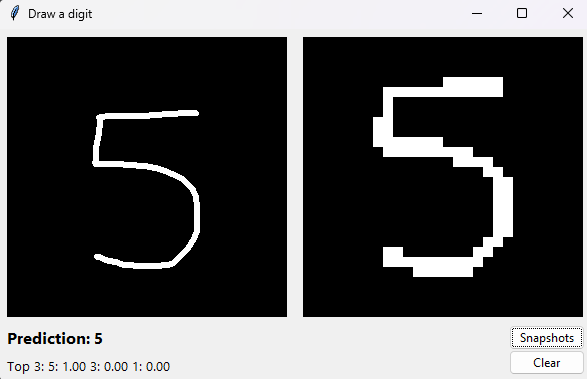
\includegraphics[width=0.45\textwidth]{mnist digit classification/5-prediction.png}
        \caption{The `Draw a digit` program predicting a drawn digit as a 5.}
        \label{fig:5 prediction}
    \end{figure}
    
    \subsubsection{Recording snapshots}

    Since we had already implemented the functionality to analyse how the neural field changed over time using snapshots,
    we decided to extend it into a useful tool that allows you to step through each iteration within the app.
    We felt that this was an important as it allows the user to visually understand how the neural field
    responds to different shapes and intensities, and how the different layers (with their own parameters) interact
    uniquely with the image.
    
    This generated an array of images (frames) that could be stitched together to produce GIF or MP4 files.
    As a result, we added an `Export as an GIF` and `Export as an MP4` in the top left menu of the snapshot window. You can view the GIF for the above digit \href{https://github.com/TheSilverLeopard/University/blob/projects/MTH2005\%20Modelling\%20-\%20Theory\%20and\%20Practice/Group\%20Project/(3-layers\%26scales-1-2-4)5-through-wilson-cowan-neural-field.gif}{here} (give a few seconds to get through the first couple of iterations).

    \section*{Conclusion}
    The Wilson-Cowan model has been studied thoroughly and key information has been used in order to analyse the Wilson-Cowan equations. These equations are studied and we find various behaviours in which it can undergo due to various parameter values and initial conditions. The model is extended to a neural field model to describe the behaviour of the system when both spatial location and time are variables. This was a key idea of the original Wilson-Cowan paper and we use this idea to greater understand the brain as it makes the model far more realistic. This allows us to model connectivity through space and find spatio-temporal patterns. We found that we are able to use machine learning with the MNIST dataset to make a feature extractor for the model. We have shown hopeful findings into the understanding of large scale brain dynamics and future research could follow on by improving computational efficiency and exploring modern machine learning techniques to further enhance performance.


\section{Contributions to the Project}

% NAME: writing - original draft of section SECTION (lead/equal), writing - review editing of section SECTION (lead/equal), investigation of section SECTION (lead/equal), visualisation of section SECTION (lead/equal), formal analysis of section SECTION (lead/equal), software - SOFTWARE_DEVELOPED (lead/equal), methodology of section SECTION (lead/equal).

Benjamin Krotowski: writing - original draft of section 1 (equal), 4, 5 (lead), writing - review editing of section 3 (equal), 4 and 5 (lead), investigation of section 1 (equal).
\newline

Andrew Jones:  writing - original draft and review editing of section 1 (equal), abstract, introduction, conclusion (lead), investigation of section 1 (equal), final read through of document (lead).
\newline

Natasha Newman: formal analysis for section 2 (lead), methodology and software for section 2 (lead), visualisation of section 2 (equal), writing - review editing of section 2 (lead), investigation of section 2 (assisted).
\newline

Rowan Broad: formal analysis of section 3 (lead), investigation of section 3 (lead), methodology and software of section 3 (lead), visualisation of section 3 (lead), writing - original draft of section 3 (lead), writing - review editing (equal).
\newline

Abby Pallot: writing - original draft of section 1 (equal), 2 (lead), writing - review editing of section 1,3 (equal), investigation of section 2 (lead), 1 (equal), visualisation of section 2 (equal), formal analysis of section 2 (assisted).
\newline

Jonas Brown: writing - original draft of sections 4.1, 6, and Appendix (lead), writing - review editing of sections 5 and 6 (lead), investigation of sections 5 (equal) and 6 (lead), visualisations of sections 5, 6 (lead), formal analysis of section 5 and 6 (lead), methodology and software of section 5 and 6 (lead).
    
    
    \section*{Appendix}
    \subsection*{Why are function calls expensive? \cite{function calls}}\label{sec:why-are-function-calls-expensive}

    Python is an interpreted language (the interpreter standardly being CPython), which at runtime must:
    \begin{itemize}
        \item Parse the source code into an abstract syntax tree (AST).
        \item Compile this into bytecode - these are a set of instructions for the computer to follow.
        \item Execute that bytecode in an evaluation loop.
    \end{itemize}
    The overhead that function calls bring are mostly in the execution stage of runtime.
    So, let us look at what happens when you call a simple function \verb|y = f(x)| during execution:
    \begin{itemize}
        \item Step 1: Evaluate the callable object \verb|f| (our function object).
        \begin{itemize}
            \item CPython looks up the name \verb|f| in each of the scopes of the program:
            \begin{itemize}
                \item \textbf{locals} - the variables within the current function, whatever that may be.
                \item \textbf{enclosing scopes} - if the current function is nested (written inside another function with local variables).
                \item \textbf{globals} - functions within the top scope (for example, constants defined at the top of the file).
                \item \textbf{builtins} - functions/global variables like \verb|range|, \verb|max|, \verb|min|, etc.
            \end{itemize}
            \item The result from this lookup \textbf{must} be a callable object since we are actively calling \verb|f| with \verb|()| parenthesis.
            \item This process is also not instant and add a cost to our function call already.
        \end{itemize}
        \item Step 2: The arguments passed, in this case \verb|x|, must then be evaluated.
        \begin{itemize}
            \item The expression within the parenthesis must is evaluated from left to right.
            \item This could mean more name lookups (like above in Step 1), attribute lookups, or indexing.
            \item The resulting argument values are then pushed onto the value stack.
            \item This is an expensive part of the execution (evaluation and pushing to the stack).
        \end{itemize}
        \item Step 3: Building a call signature.
        \begin{itemize}
            \item \verb|f(x)| - creates a simple array of arguments.
            \item \verb|f(x, y=3)| - builds a map of the keyword names (kwargs) to values (args).
            \item \verb|f(*arg, **kwargs)| - unpacks mappings.
        \end{itemize}
        \item Step 4: Actually call the function - this uses a generic call structure.
        \begin{itemize}
            \item Checks if the object (\verb|f|) is callable (if it is a function).
            \item Finds the appropriate entry (where to start execution from) to the function.
            \item Fortunately, builtins are specifically made to be fast (using special routing) and use C-based methods, so these are less expensive to call.
        \end{itemize}
        \item Step 5: Creates a new, rather expensive, stack frame. This is an environment for the function to run within, containing:
        \begin{itemize}
            \item An instruction pointer - this tracks your position in the bytecode.
            \item Local variables - this is for fast lookups described partly in Step 2.
            \item Global/builtin references - so the function isn't limited to the local scope.
            \item An evaluation stack.
            \item Exception handling information.
        \end{itemize}
        \item Step 6: Binds arguments to parameters.
        \begin{itemize}
            \item CPython maps these onto the function's parameters:
            \begin{itemize}
                \item Positional parameters.
                \item Keyword-only parameters.
                \item Default values.
                \item args and kwargs.
            \end{itemize}
            \item While also checking for errors:
            \begin{itemize}
                \item Missing required arguments.
                \item Unexpected arguments/keywords.
                \item Other general checks.
            \end{itemize}
        \end{itemize}
        \item Step 7: Finally start to execute the bytecode.
        \begin{itemize}
            \item Initialisation of local variables.
            \item Execution begins at the address of the entry point for \verb|f|.
            \item CPython starts a bytecode evaluation loop for this new frame:
            \begin{itemize}
                \item Fetch the next bytecode instruction.
                \item Decode instruction into an opcode.
                \item Dispatch (jump) to a C code implementation of that opcode.
                \item Manipulate the value stack to reflect result of operation.
                \item Increment the instruction pointer and repeat.
            \end{itemize}
        \end{itemize}
        \item Step 8: Create return value and teardown frame.
        \begin{itemize}
            \item Produces a return value object if necessary.
            \item Removes the frame from the call stack.
            \item Restores calling frame back to the current frame.
            \item Pushes the return value onto the caller's evaluation stack.
        \end{itemize}
        \item Step 9: Assign result to \verb|y| - updates the local scope binding (of the calling scope) of \verb|y|.
    \end{itemize}
    Comparing with the steps for inline arithmetic, for example with \verb|y = x*x + 2|:
    \begin{itemize}
        \item Fetch next bytecode instruction.
        \item Lookup \verb|x|, which is found within the \textbf{locals} array (this is the first lookup array, so extremely fast), and push the value of \verb|x| onto the value stack.
        \\ \verb|stack = [x]|
        \item Lookup \verb|x| a second time and push onto the stack.
        \\ \verb|stack = [x, x]|
        \item Multiply \verb|x * x|.
        \begin{itemize}
            \item Pop top two items from stack (\verb|x| and \verb|x|).
            \\ \verb|stack = []|
            \item Determine the correct multiplication operation for the runtime type of the variables (\verb|int|, \verb|float|, etc.).
            \item Dispatch to a C code implementation (multiplication in this case).
            \item Push result onto the stack.
            \\ \verb|stack = [x_squared]|
        \end{itemize}
        \item Load \verb|2| and push onto the stack.
        \\ \verb|stack = [x_squared, 2]|
        \item Add \verb|x_squared + 2|.
        \begin{itemize}
            \item Pop top two items from stack (\verb|x_squared| and \verb|2|).
            \\ \verb|stack = []|
            \item Determine the correct addition operation for the runtime type of the variables (\verb|int|, \verb|float|, etc.).
            \item Dispatch to a C code implementation (addition in this case).
            \item Push result onto the stack.
            \\ \verb|stack = [result]|
        \end{itemize}
        \item Store result into \verb|y|.
        \begin{itemize}
            \item Pop top item from stack (\verb|result|).
            \\ \verb|stack = []|
            \item Store \verb|result| in \verb|y|.
        \end{itemize}
    \end{itemize}
    
    As you can see, inline arithmetic is much cheaper for the CPU as it does not require argument evaluation,
    building call signatures, stack frame creation, binding of arguments, error handling, or creation of return values.
    These are all relatively expensive operations and should be considered when choosing methods or algorithms when large amounts
    of data or iterations are required.

    
    \subsection*{Graphs}

\noindent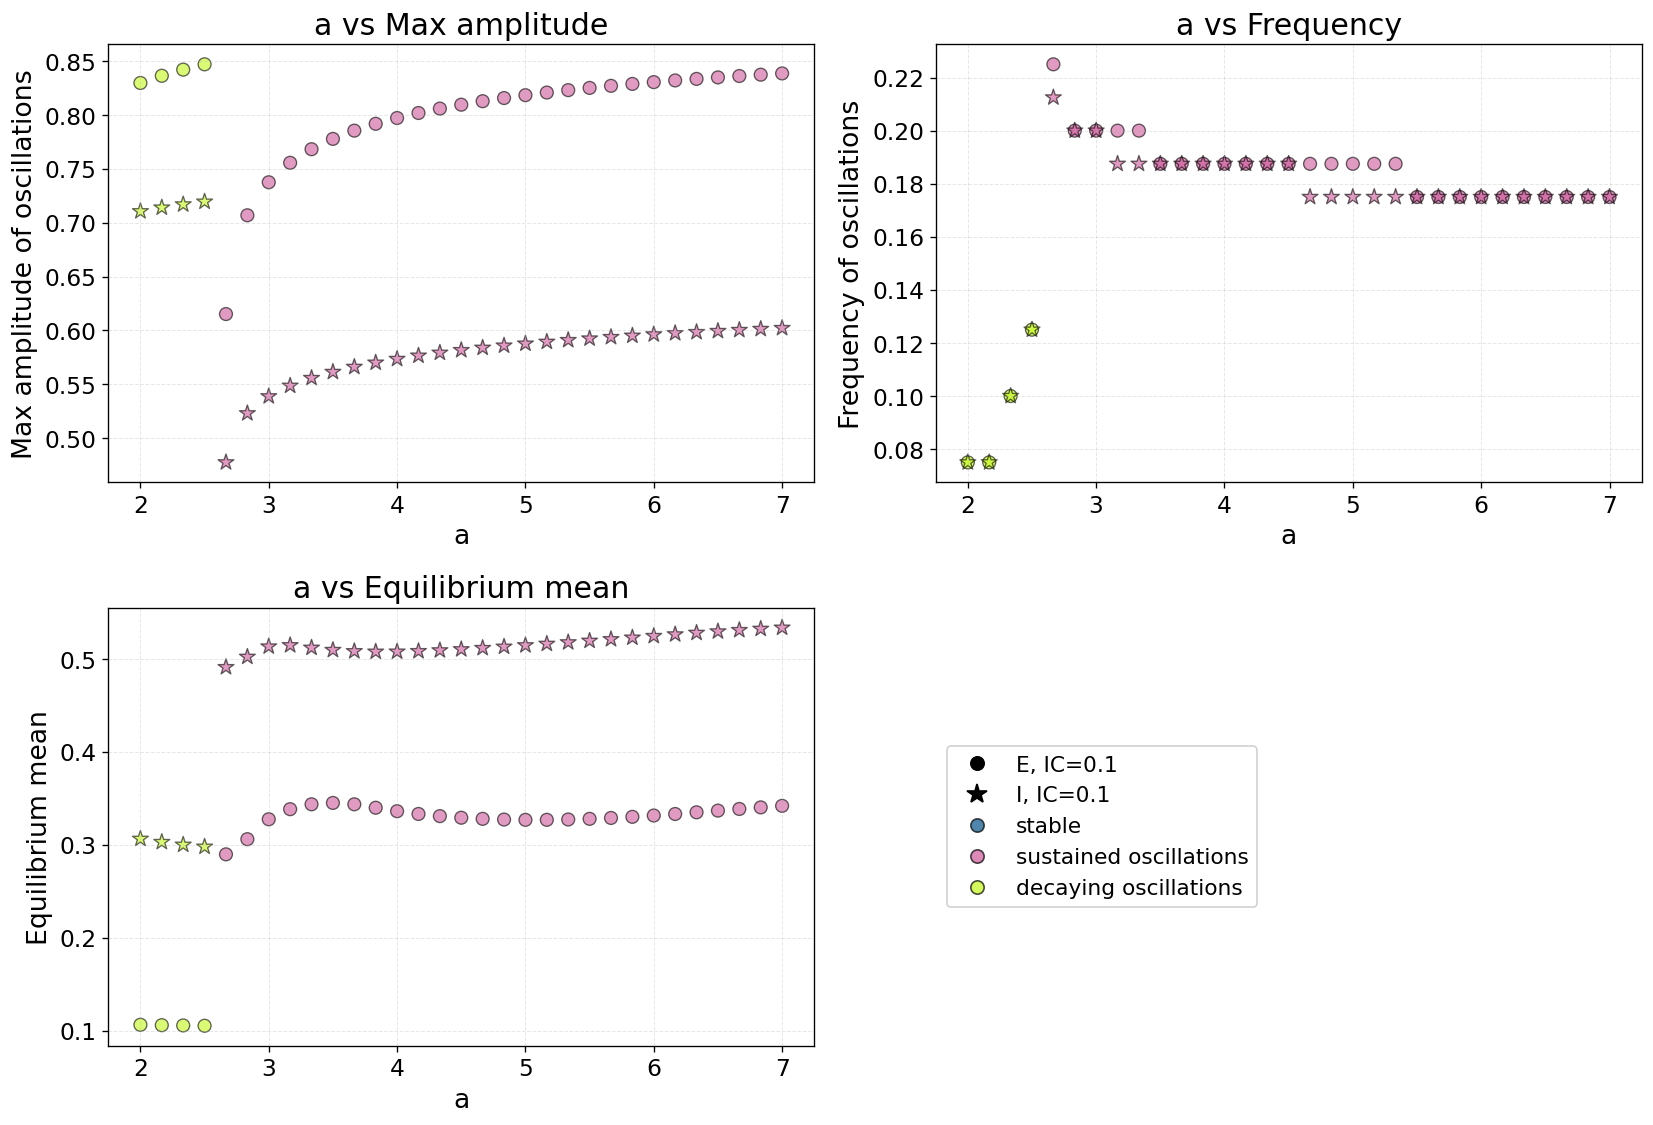
\includegraphics[width=\linewidth]{param graphs/a.png}
\captionof{figure}{a sweep for ICs = (0.1, 0.1)}
\label{a graphs}

\noindent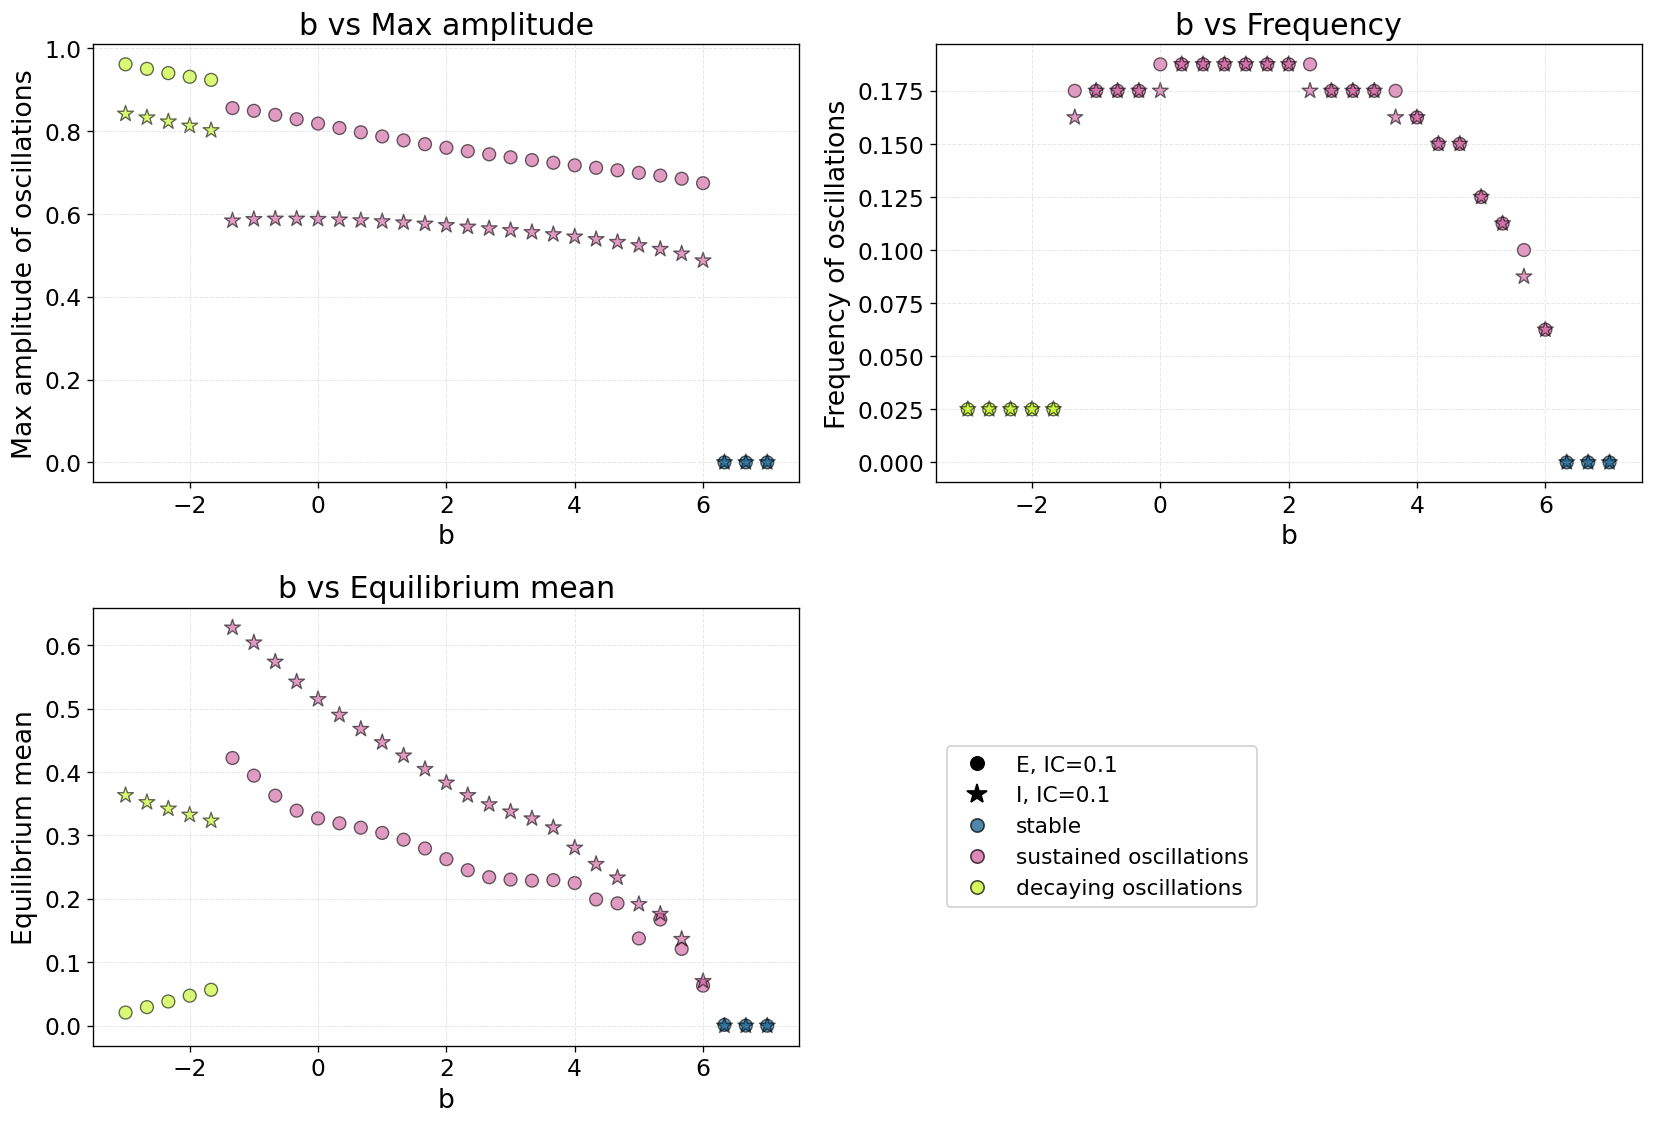
\includegraphics[width=\linewidth]{param graphs/b.png}
\captionof{figure}{b sweep for ICs = (0.1, 0.1)}
\label{b graphs}

\noindent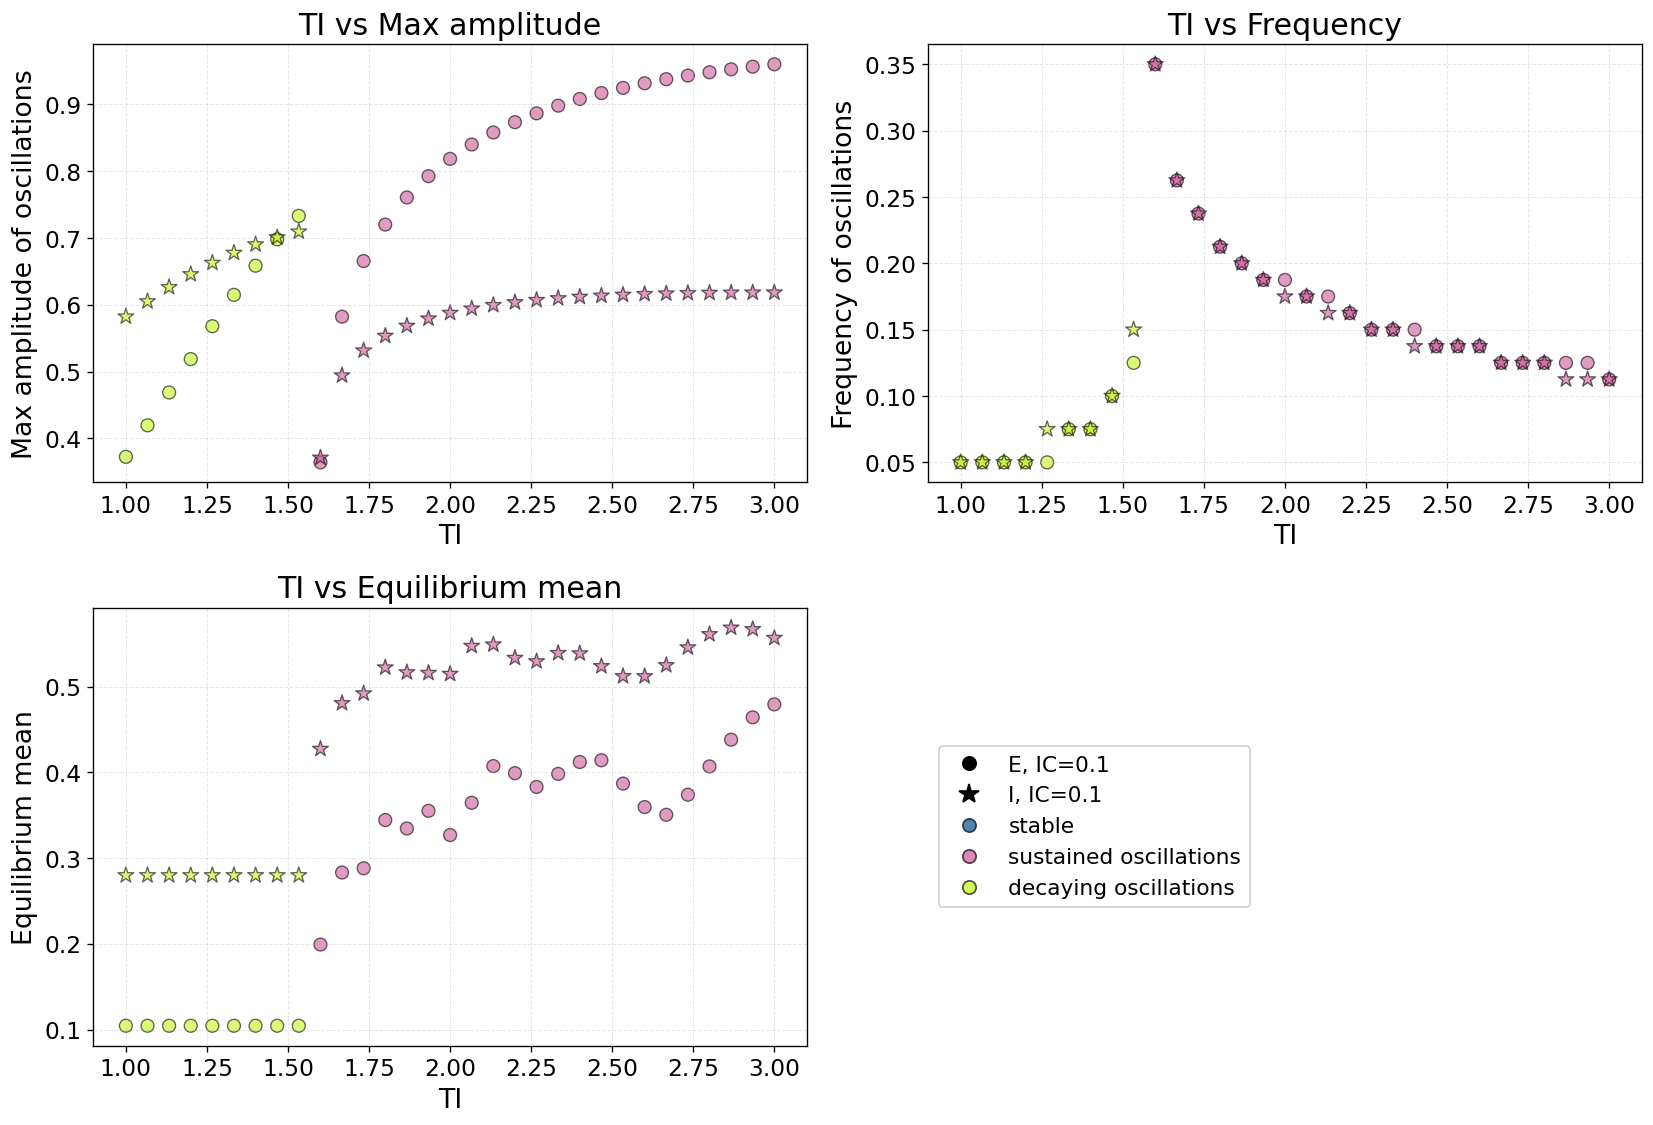
\includegraphics[width=\linewidth]{param graphs/TI.png}
\captionof{figure}{TI sweep for ICs = (0.1, 0.1)}
\label{TI graphs}

\noindent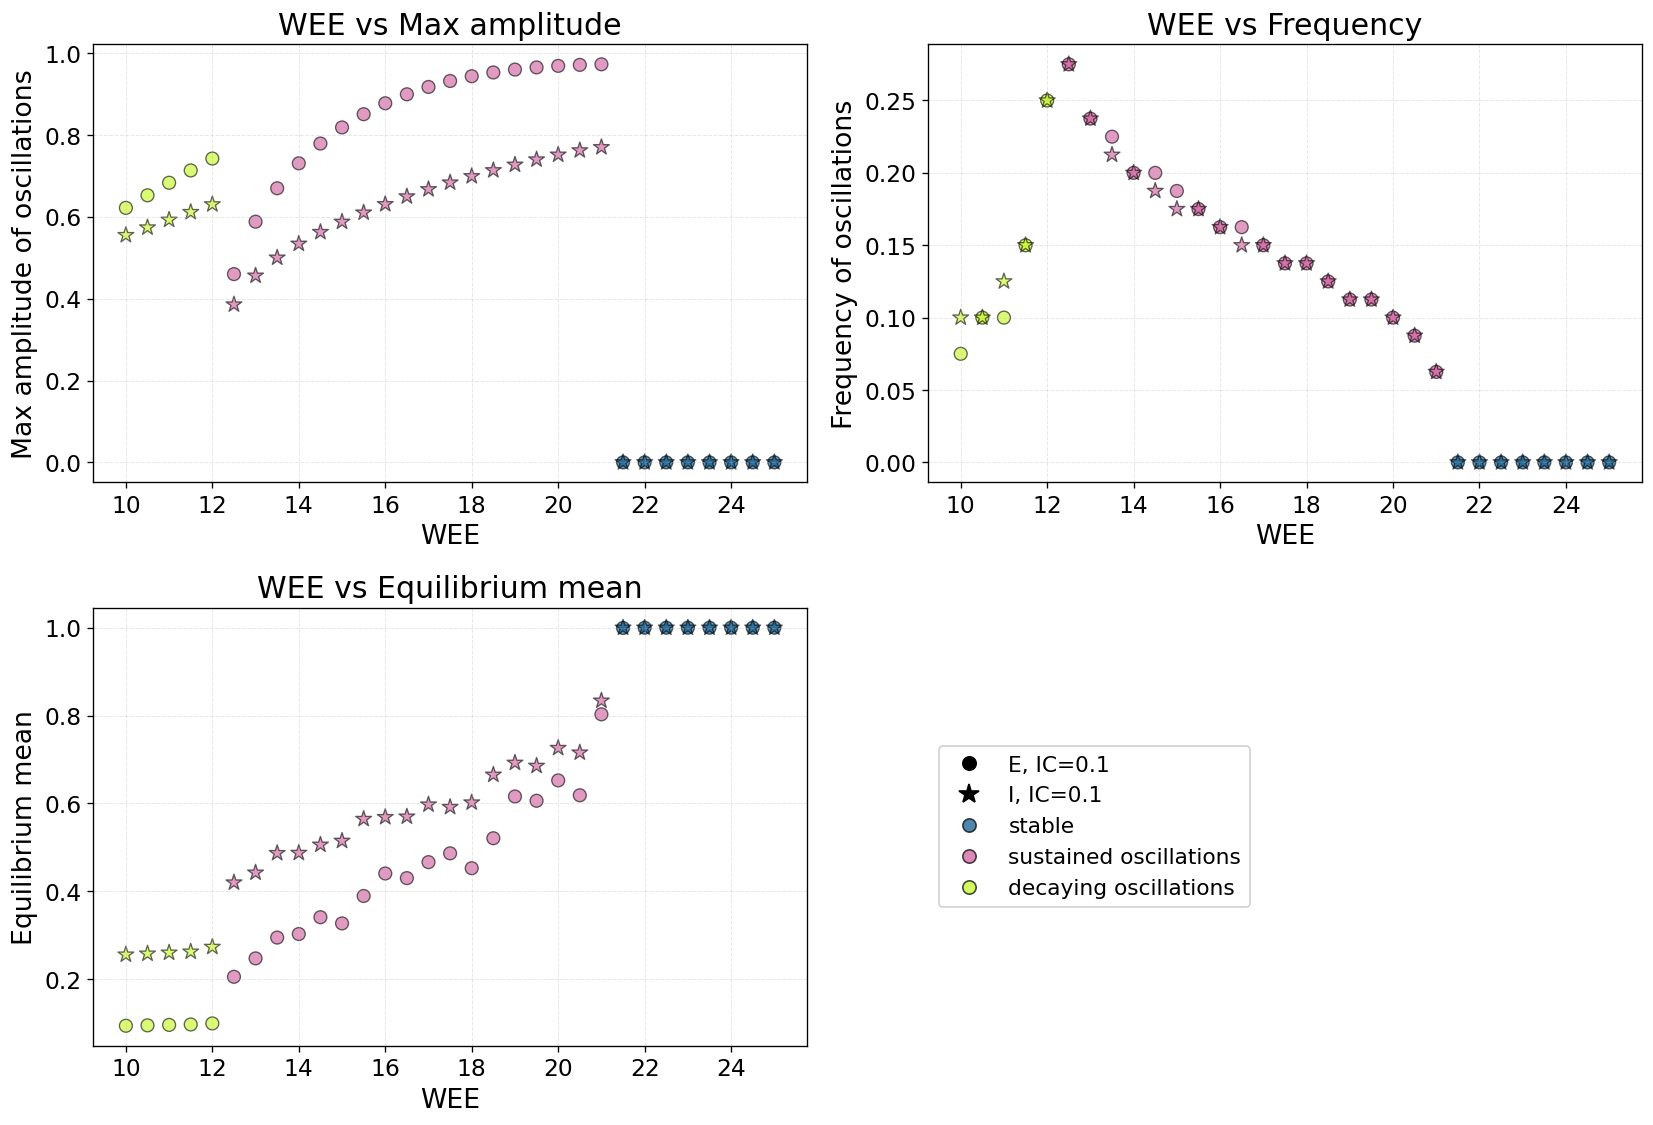
\includegraphics[width=\linewidth]{param graphs/WEE.png}
\captionof{figure}{WEE sweep for ICs = (0.1, 0.1)}
\label{WEE graphs}

\noindent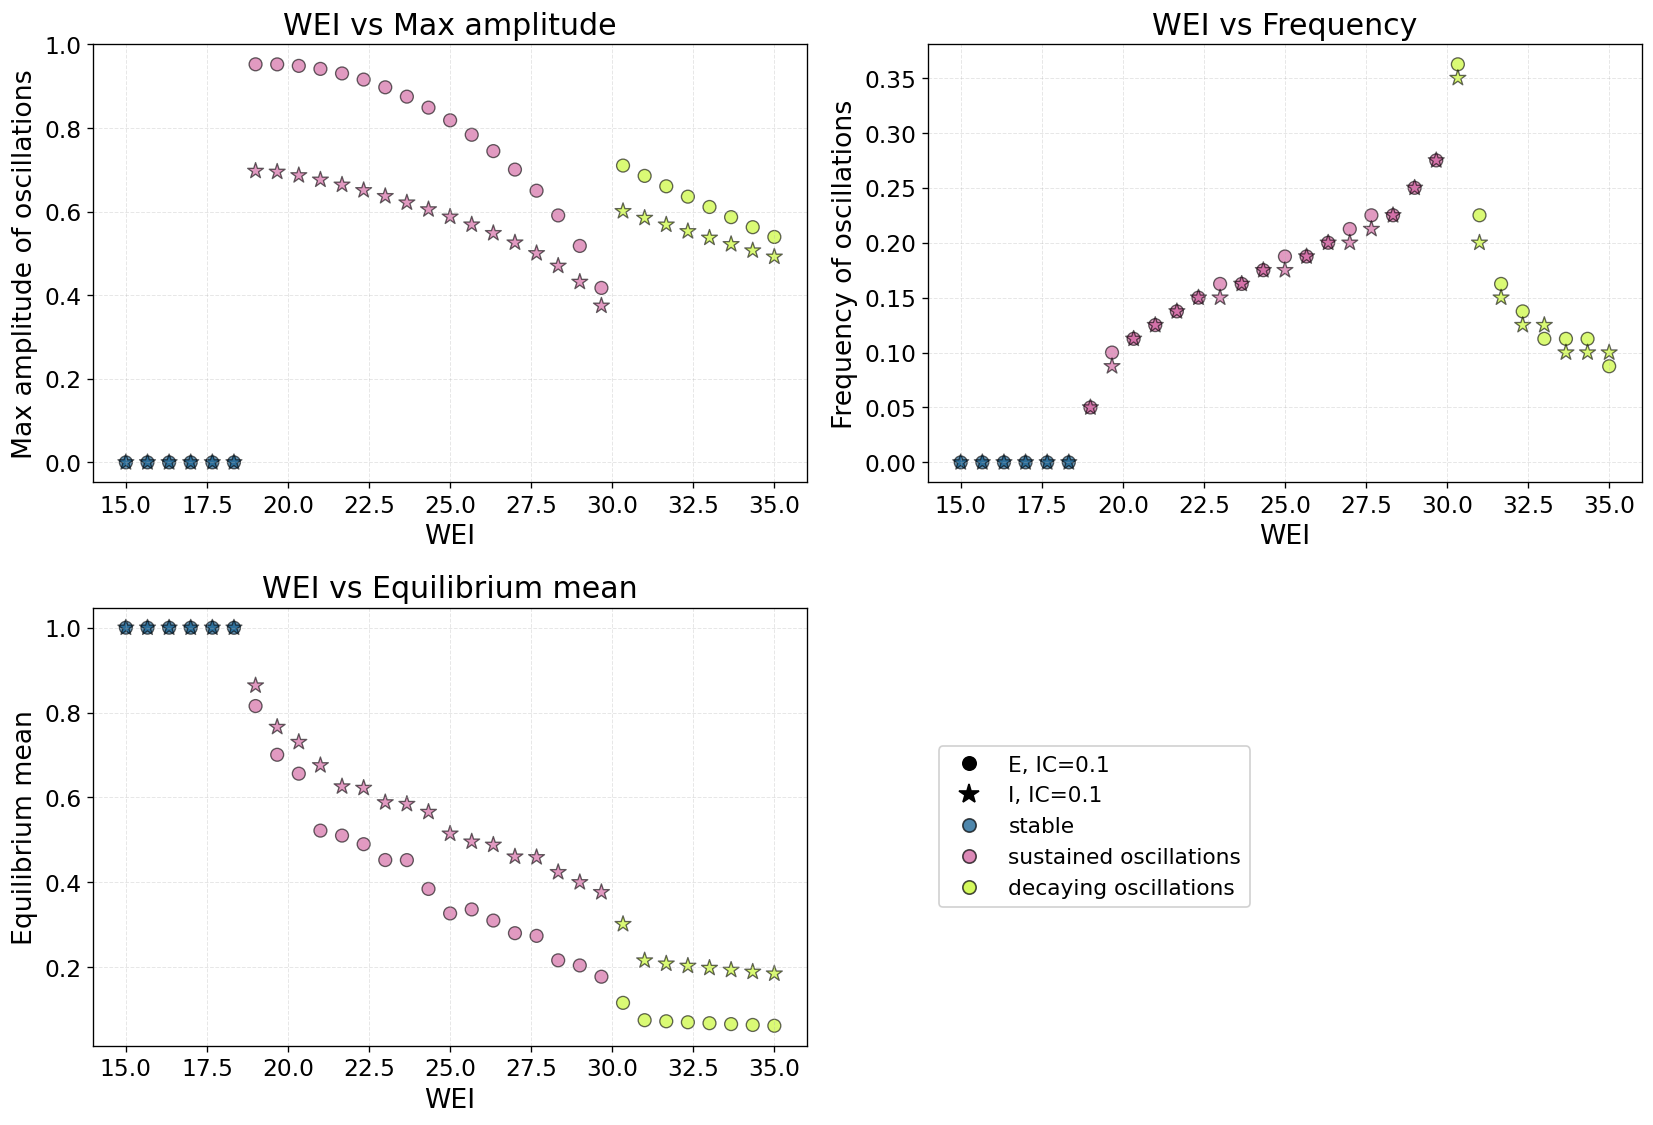
\includegraphics[width=\linewidth]{param graphs/WEI.png}
\captionof{figure}{WEI sweep for ICs = (0.1, 0.1)}
\label{WEI graphs}

\noindent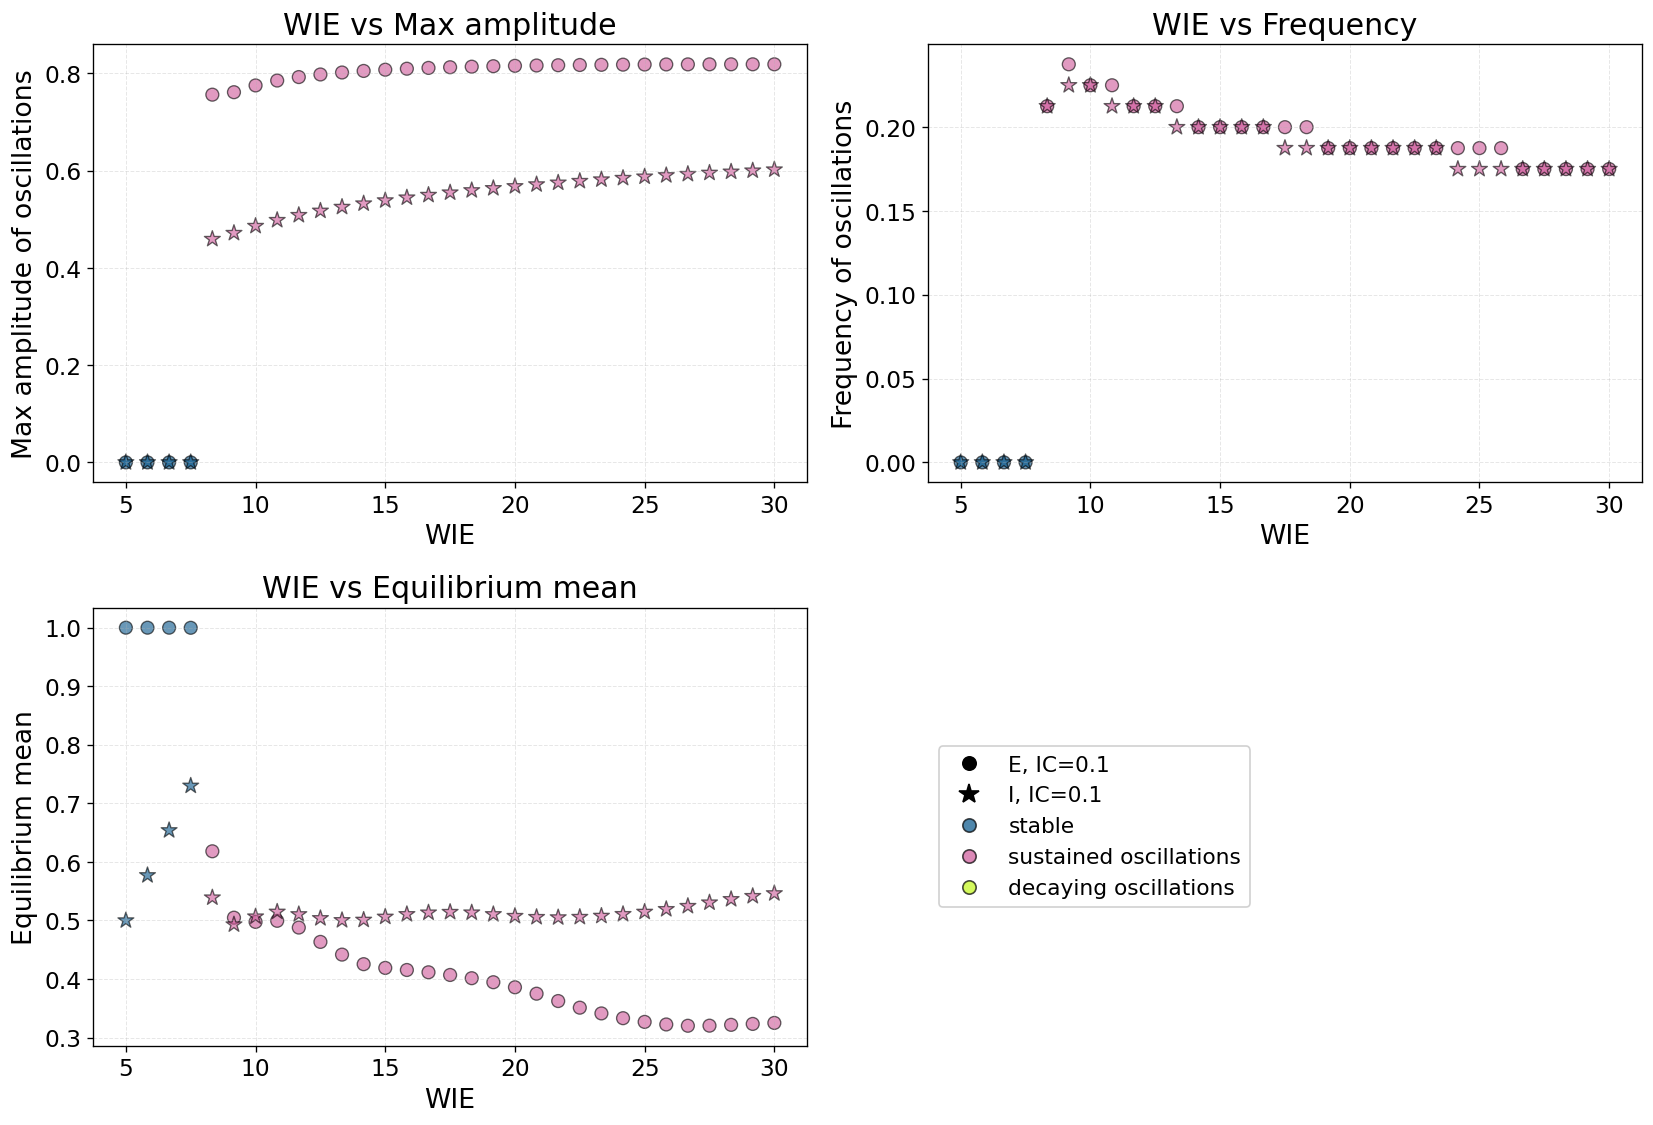
\includegraphics[width=\linewidth]{param graphs/WIE.png}
\captionof{figure}{WIE sweep for ICs = (0.1, 0.1)}
\label{WIE graphs}

\noindent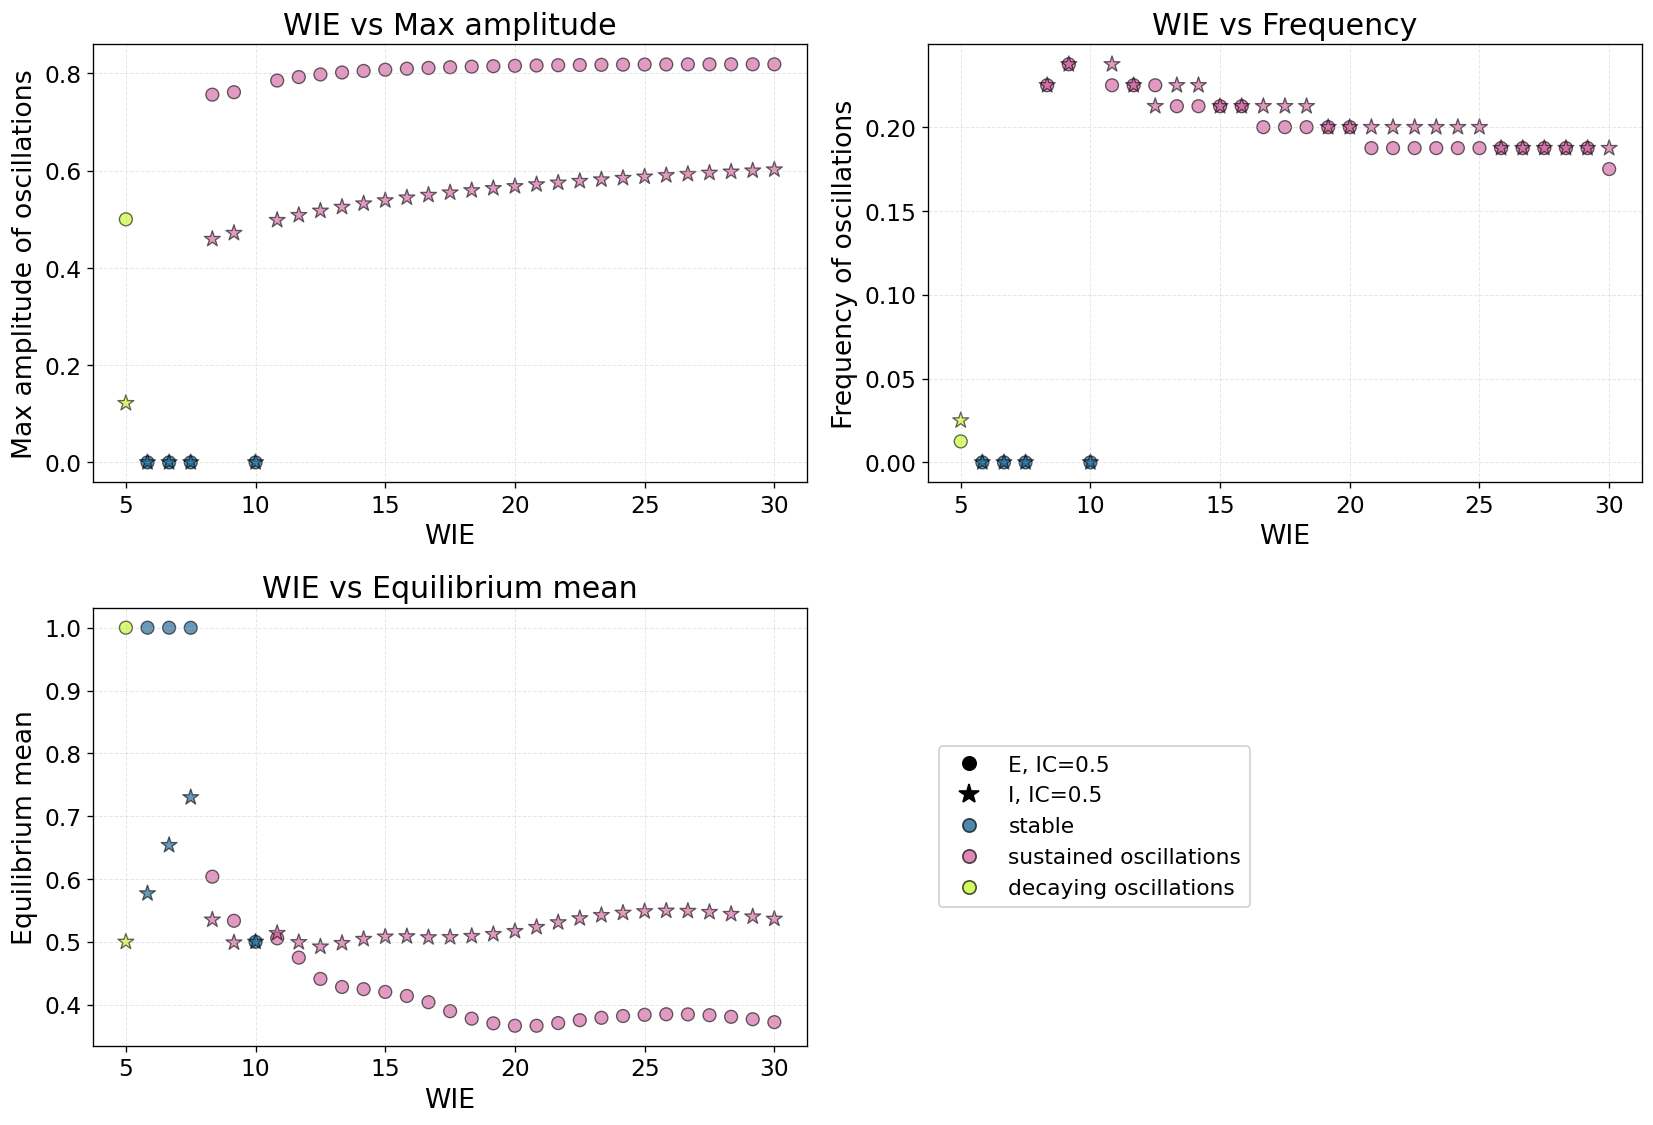
\includegraphics[width=\linewidth]{param graphs/WIE 0.5 0.5.png}
\captionof{figure}{WIE sweep for ICs = (0.5, 0.5)}
\label{WIE 0.5 0.5}

\noindent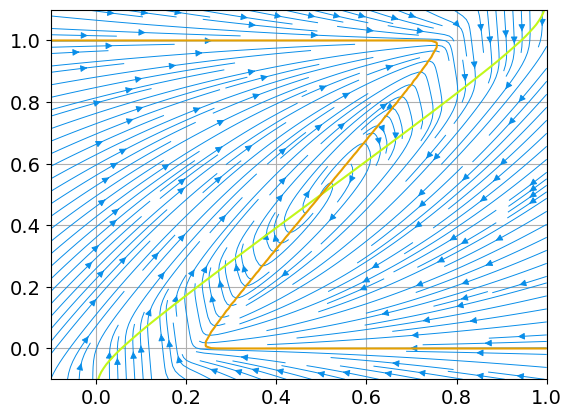
\includegraphics[width=\linewidth]{param graphs/WIE = 10 streamplot.png}
\captionof{figure}{WIE = 10 streamplot}
\label{WIE = 10}

\noindent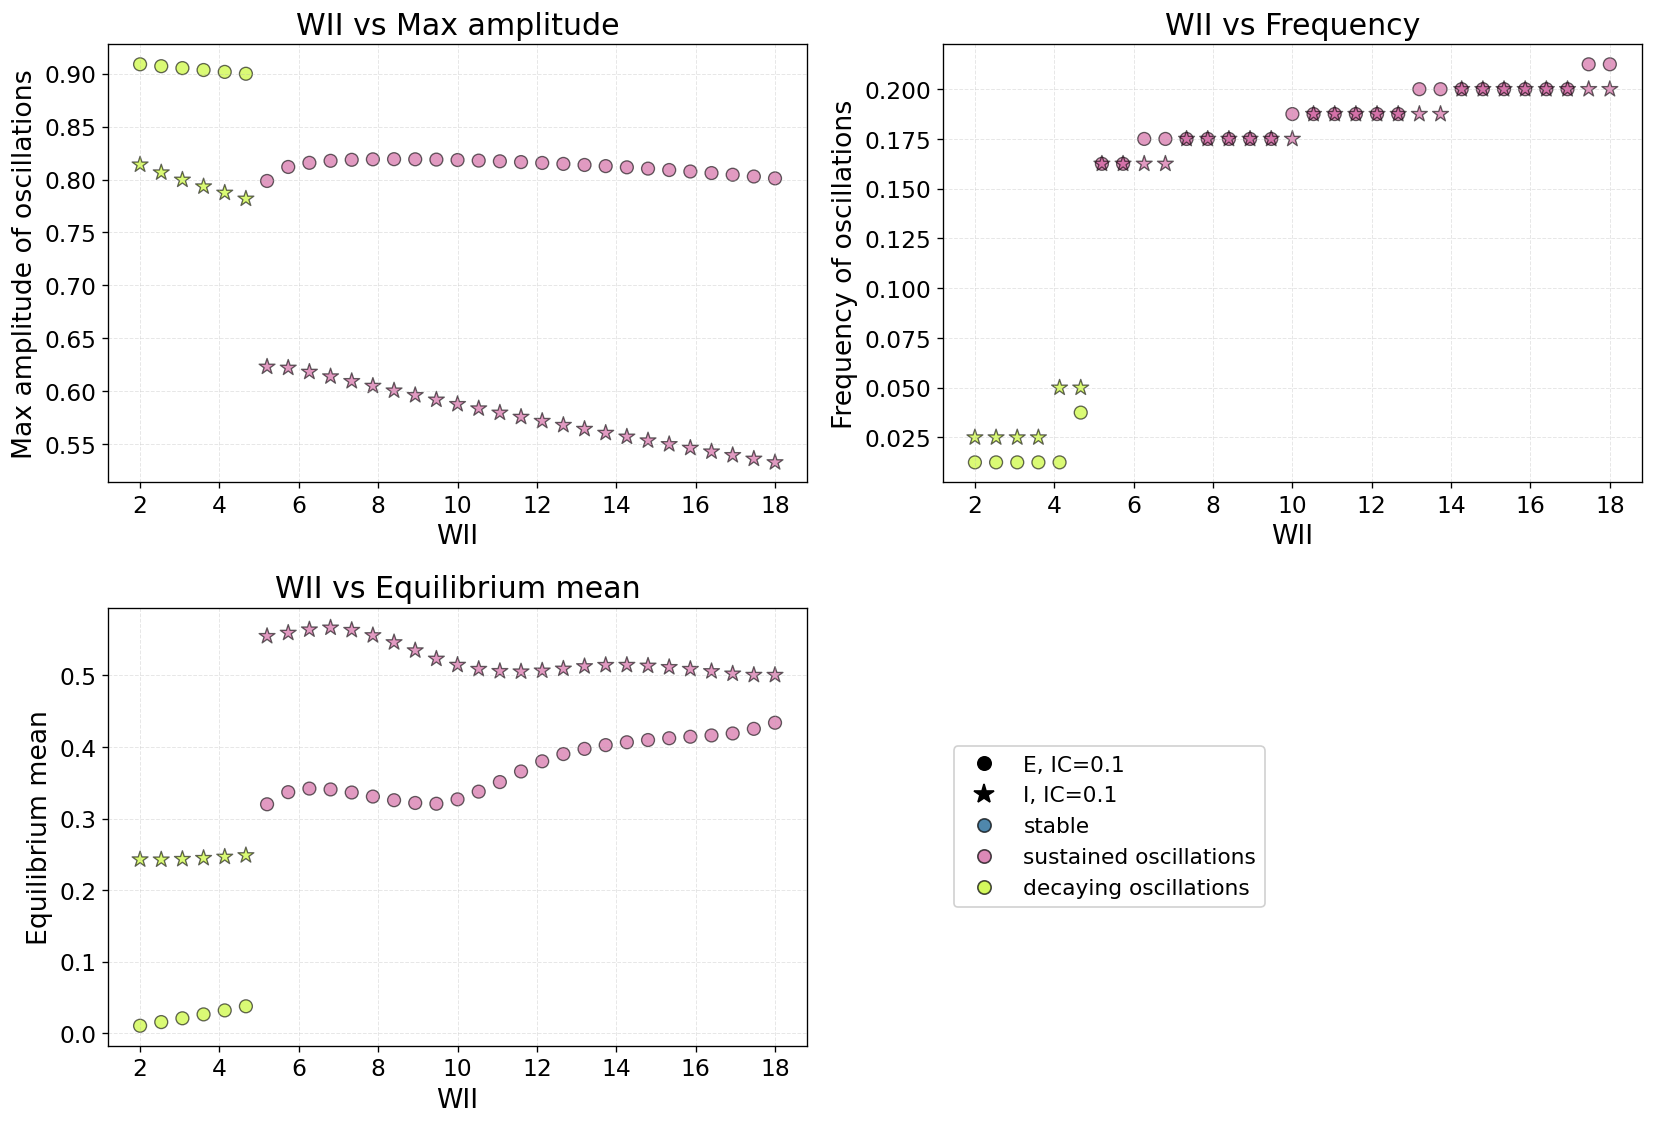
\includegraphics[width=\linewidth]{param graphs/WII.png}
\captionof{figure}{WII sweep for ICs = (0.1, 0.1)}
\label{WII graphs}

\noindent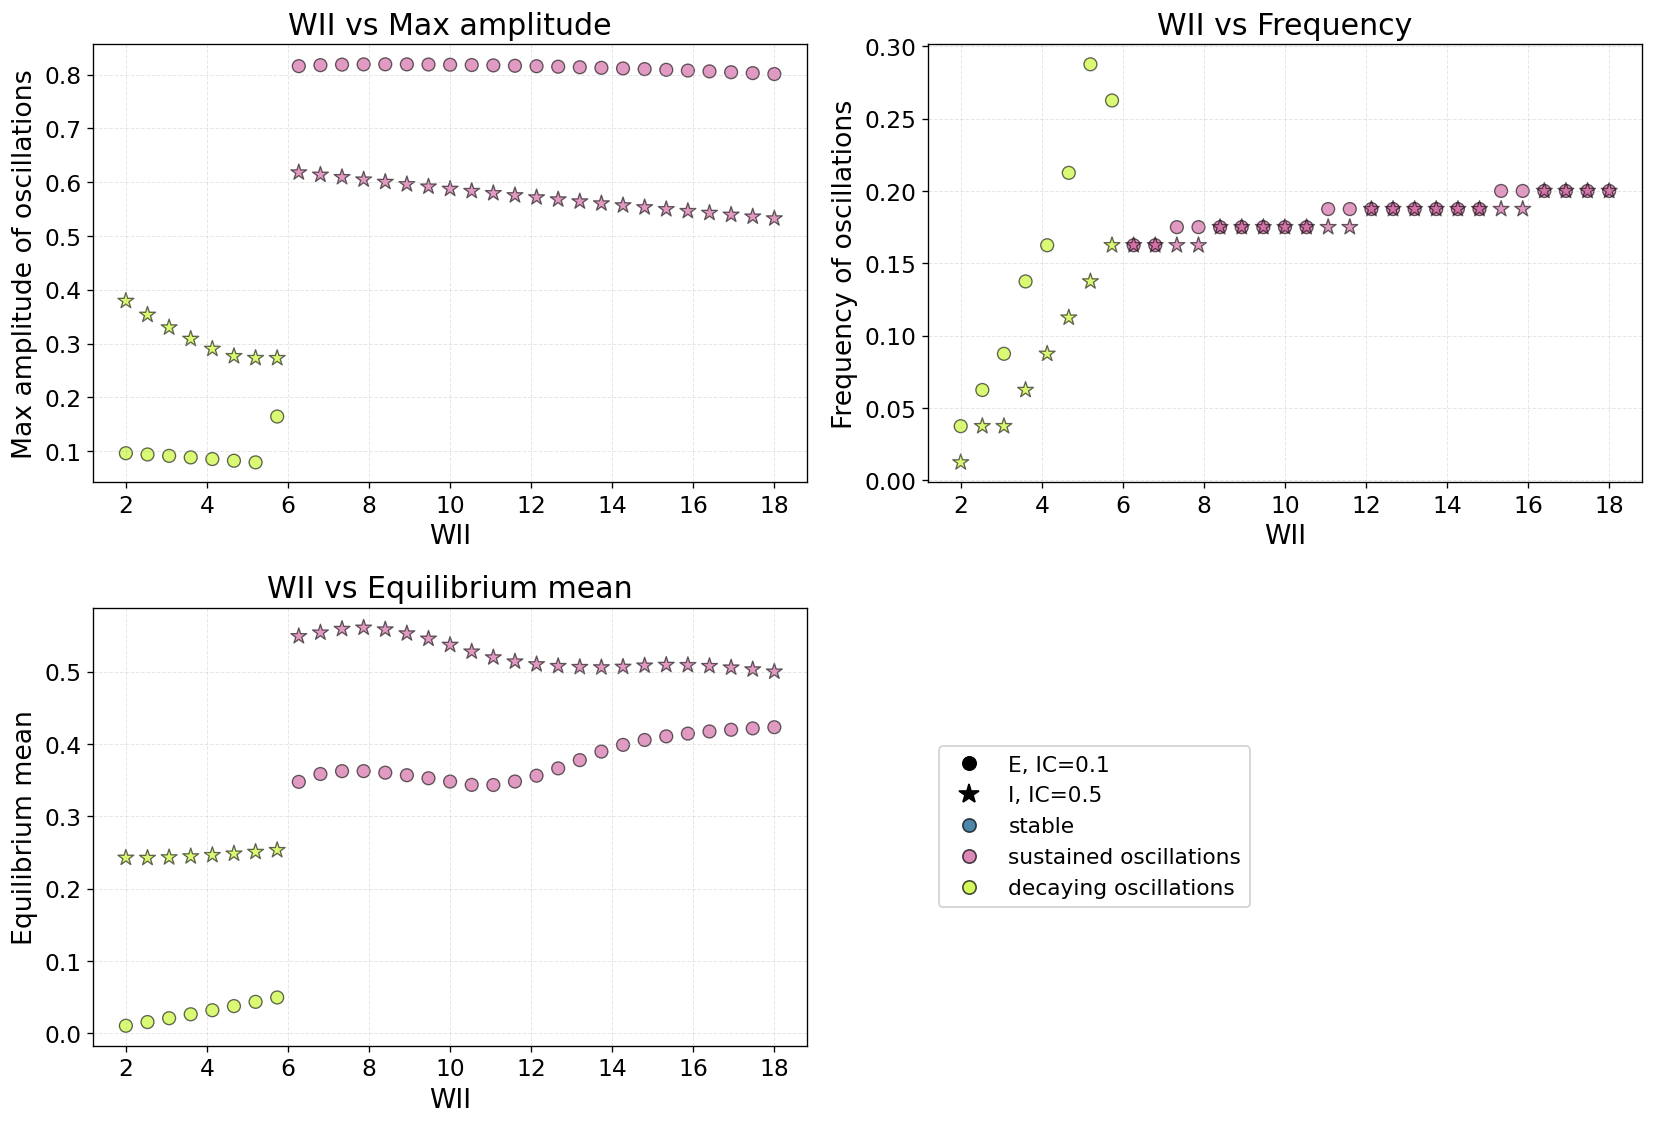
\includegraphics[width=\linewidth]{param graphs/WII 0.1_0.5.png}
\captionof{figure}{WII sweep for ICs = (0.1, 0.5)}
\label{WII graphs 0.1 0.5}

\noindent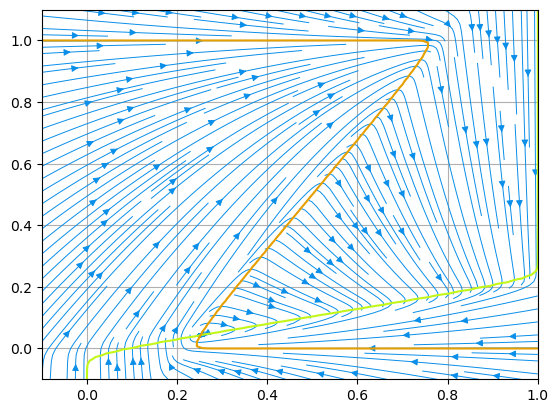
\includegraphics[width=\linewidth]{param graphs/WII = 5.2.png}
\captionof{figure}{Phase plot for WII = 5.2}
\label{WII = 5.2}

\noindent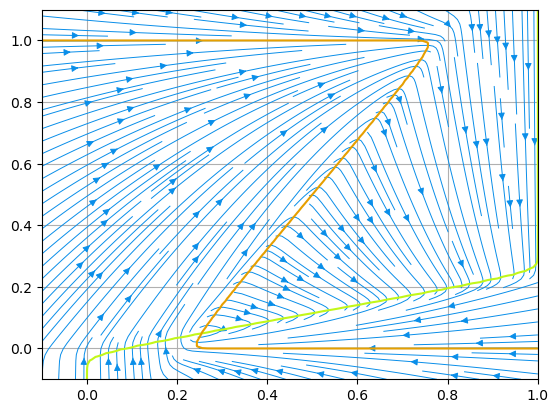
\includegraphics[width=\linewidth]{param graphs/WII = 5.73.png}
\captionof{figure}{Phase plot for WII = 5.73}
\label{WII = 5.73}

\noindent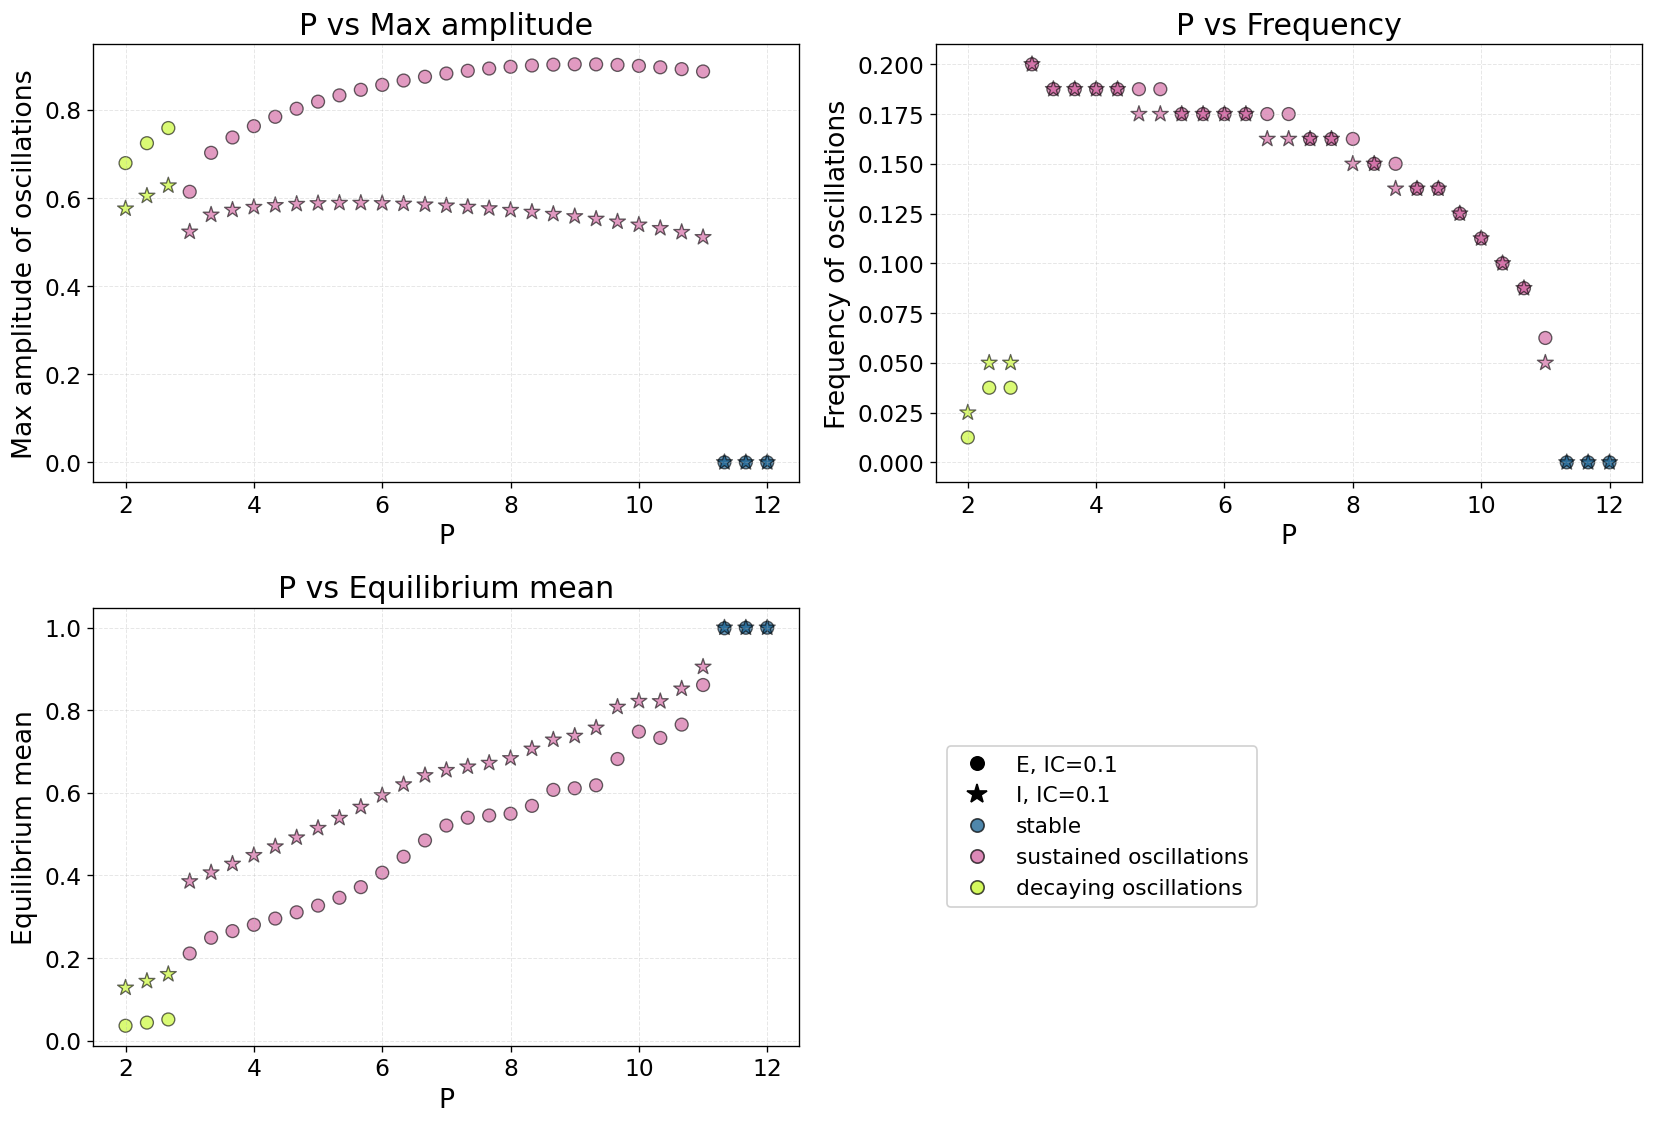
\includegraphics[width=\linewidth]{param graphs/P.png}
\captionof{figure}{P sweep for ICs = (0.1, 0.1)}
\label{P graphs}

\noindent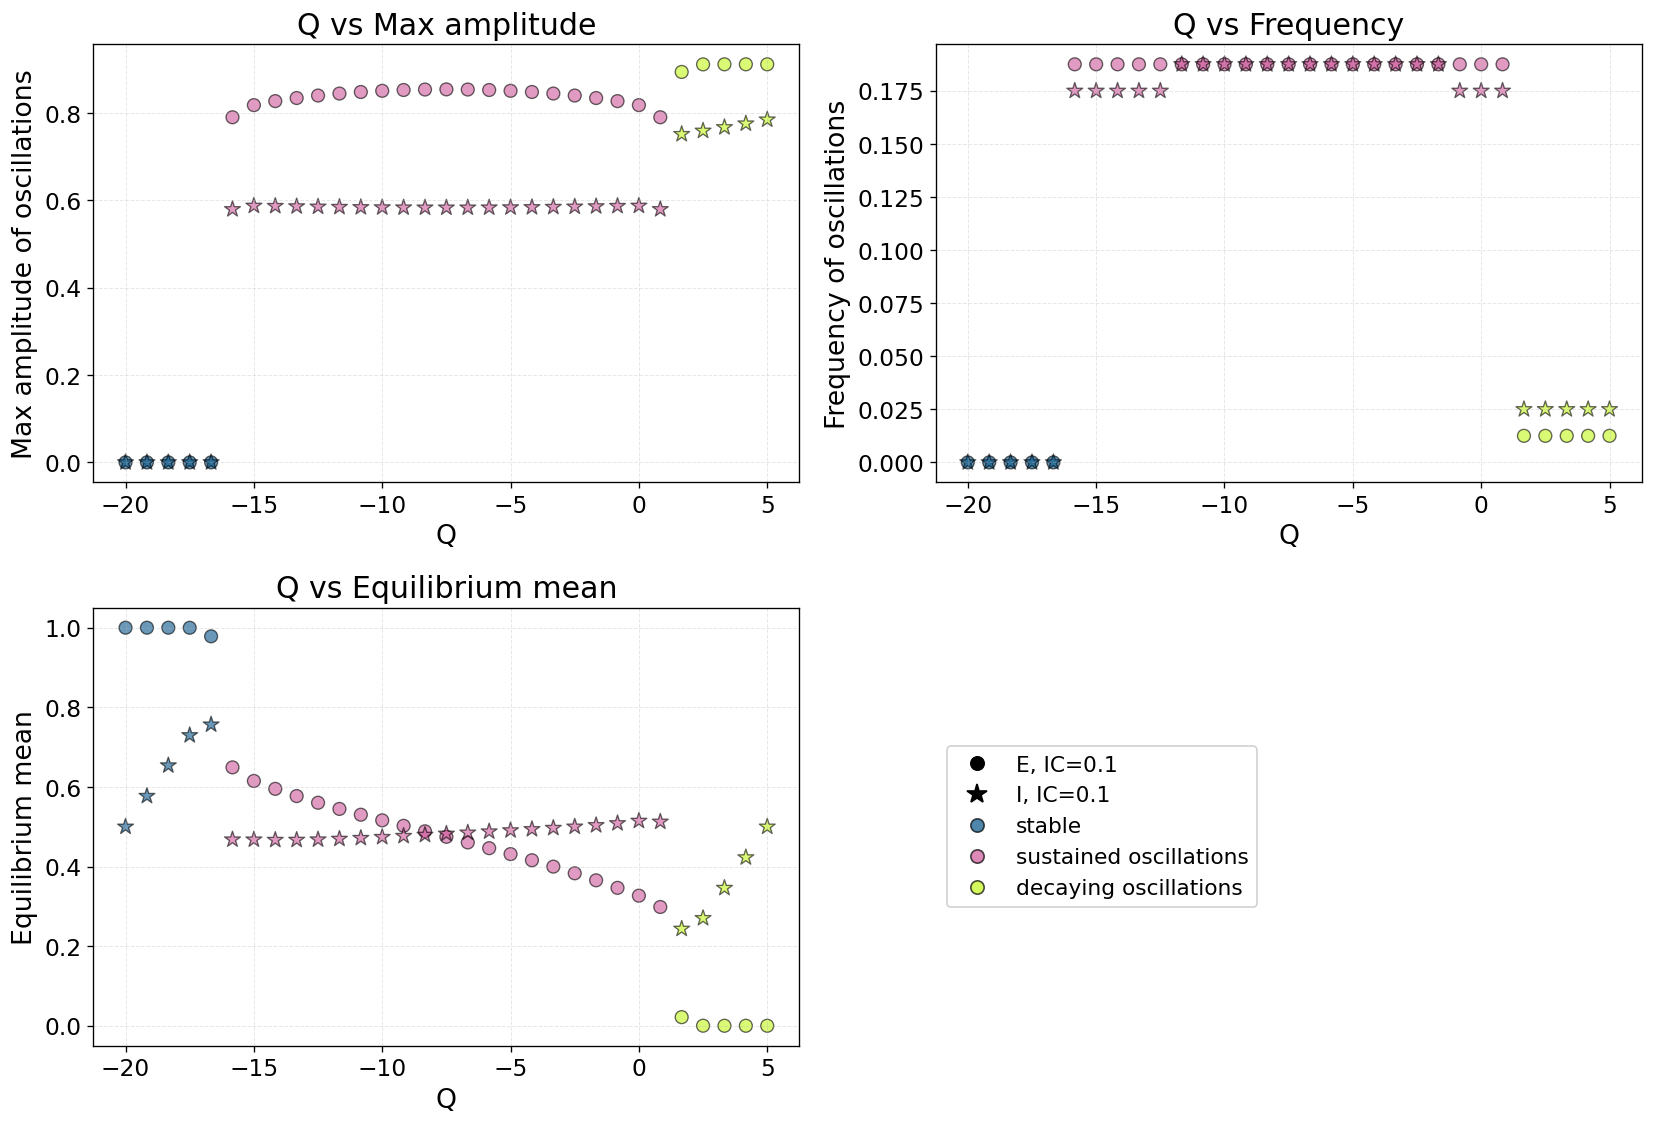
\includegraphics[width=\linewidth]{param graphs/Q.png}
\captionof{figure}{Q sweep for ICs = (0.1, 0.1)}
\label{Q graphs}

\noindent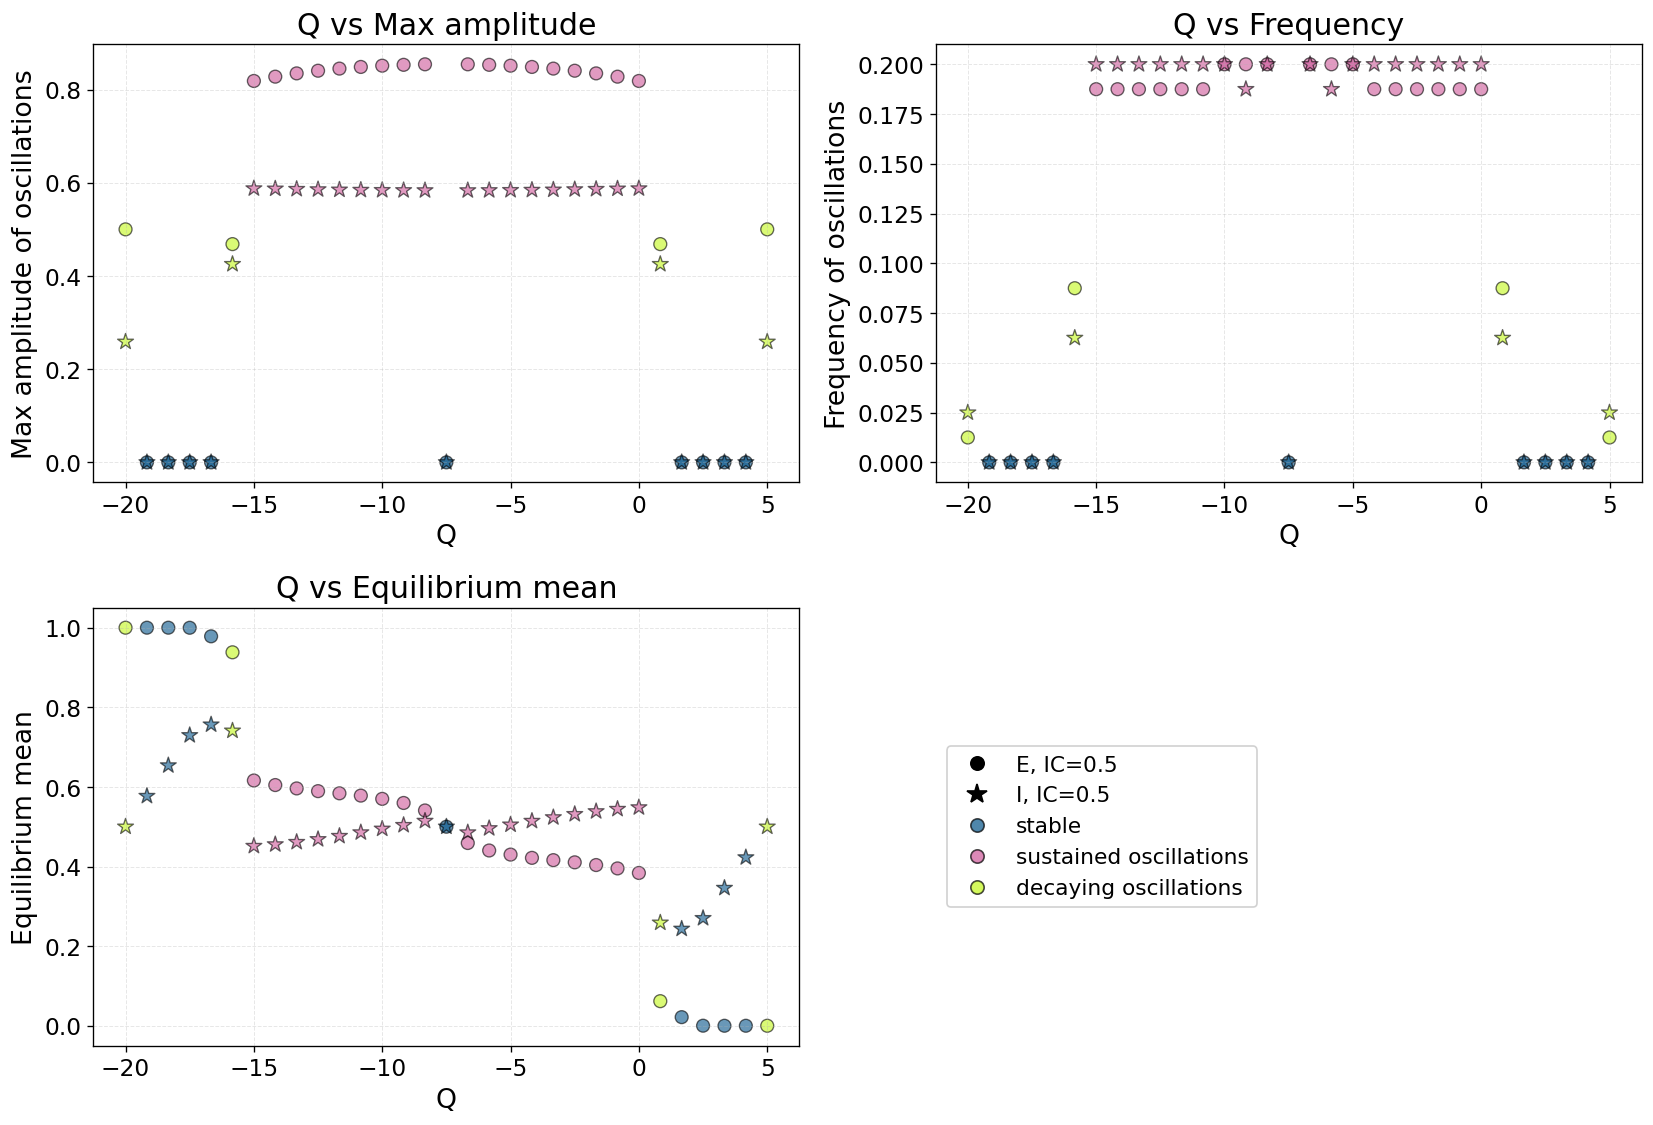
\includegraphics[width=\linewidth]{param graphs/Q 0.5_0.5.png}
\captionof{figure}{Q sweep for ICs = (0.5, 0.5)}
\label{Q 0.5 0.5}

\noindent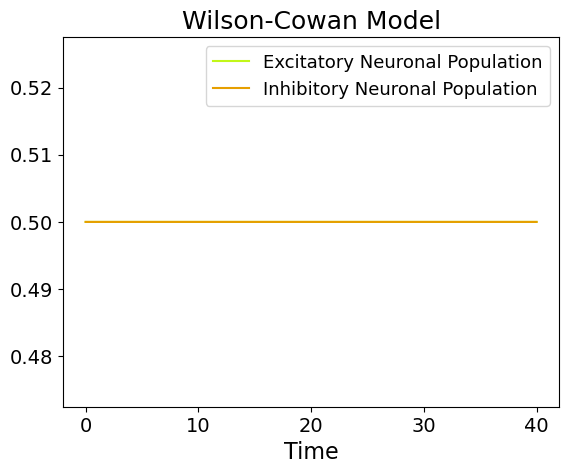
\includegraphics[width=\linewidth]{param graphs/Q = -7.5 timeseries.png}
\captionof{figure}{Q = -7.5 timeseries}
\label{Q = -7.5 timeseries}

\noindent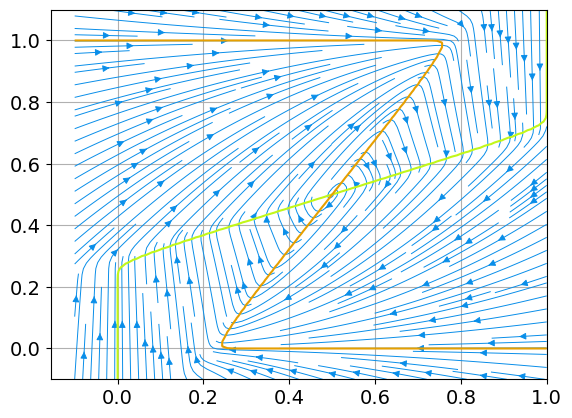
\includegraphics[width=\linewidth]{param graphs/Q = -7.5 streamplot.png}
\captionof{figure}{Q = -7.5 streamplot}
\label{Q = -7.5 streamplots}

\noindent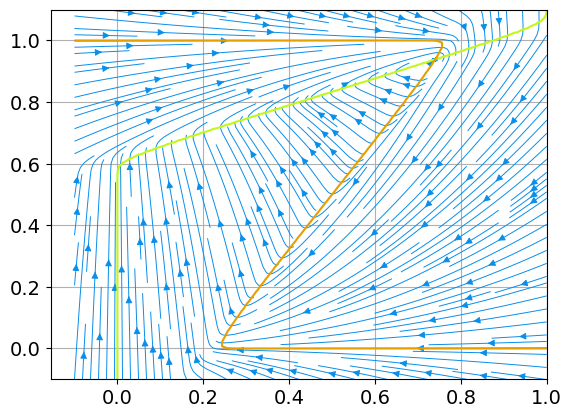
\includegraphics[width=\linewidth]{param graphs/Q = -15.833 streamplot.png}
\captionof{figure}{Q = -15.833 streamplot}
\label{Q = -15.833 streamplot}

\noindent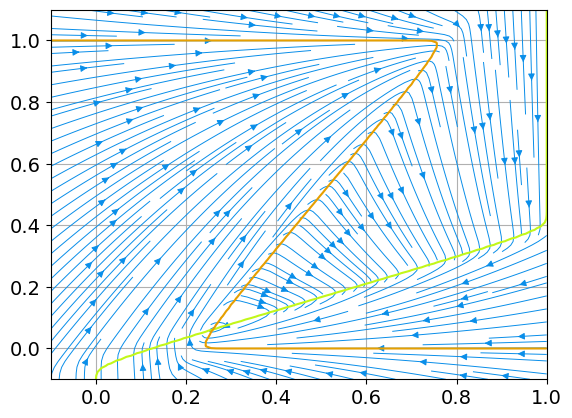
\includegraphics[width=\linewidth]{param graphs/Q = 0.83 streamplot.png}
\captionof{figure}{Q = 0.83 streamplot}
\label{Q = 0.83 streamplot}

\subsection*{Bob}

\begin{center}
    \noindent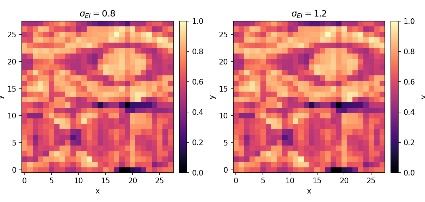
\includegraphics[width=0.4\linewidth]{Heatmaps/bob_initial.png}
    \qquad
    \noindent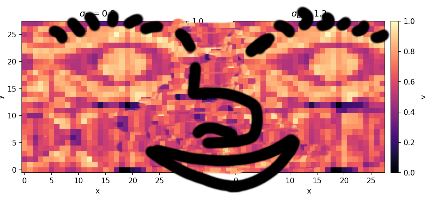
\includegraphics[width=0.4\linewidth]{Heatmaps/bob.png}
    \captionof{figure}{\textbf{Bob} - accidentally discovered within bugged code with sub-matrices $W_{EI}$ and $W_{II}$ not transposed (needed for batching) and a Gaussian kernel without the Mexican-hat shape - edited with joy.}
    \label{bob plot}
\end{center}


% https://en.wikipedia.org/wiki/Wilson%E2%80%93Cowan_model
\begin{thebibliography}{99}

\bibitem{PnQ}
Wilson, H.R., Cowan, J.D. A mathematical theory of the functional dynamics of cortical and thalamic nervous tissue. Kybernetik 13, 55–80 (1973). \url{https://doi.org/10.1007/BF00288786}

\bibitem{EVO}
Wilson, H.R., Cowan, J.D. Evolution of the Wilson–Cowan equations. Biol Cybern 115, 643–653 (2021). \url{https://doi.org/10.1007/s00422-021-00912-7}

\bibitem{wiki}
Wikipedia Wilson–Cowan model  \url{https://en.wikipedia.org/w/index.php?title=Wilson%E2%80%93Cowan_model&oldid=1323572024}

\bibitem{WC}
Tutorial 2: Wilson-Cowan Model — Neuromatch Academy: Computational Neuroscience (Accessed: 04 March 2026). \url{https://compneuro.neuromatch.io/tutorials/W2D4_DynamicNetworks/student/W2D4_Tutorial2.html}
(Upon final review link is now broken, but was active when accessed)

\bibitem{oscillation}
Godin, C., Krause, M.R., Vieira, P.G., Pack, C.C., Thivierge, J.-P. Control of Inhibition-Stabilized Oscillations in Wilson-Cowan Networks with Homeostatic Plasticity. Entropy (2025), 27, 215. \url{https://doi.org/10.3390/e27020215}

\bibitem{journal}
de Candia, A., Sarracino, A., Apicella, I., de Arcangelis, L. Critical behaviour of the stochastic Wilson-Cowan model (2021).
\url{https://journals.plos.org/ploscompbiol/article?id=10.1371/journal.pcbi.1008884}

\bibitem{hi}
Wilson, H.R., Cowan, J.D. Excitatory and inhibitory interactions in localized populations of model neurons (1972). \url{https://doi.org/10.1016/S0006-3495(72)86068-5}

\bibitem{Oshima}
Noebels J.L., Avoli M., Rogawski M.A., et al., editors.
New York: Oxford University Press. Jasper's Basic Mechanisms of the Epilepsies. 5th edition (2024). doi: 10.1093/med/9780197549469.002.0007
\url{https://www.ncbi.nlm.nih.gov/books/NBK609860/}

\bibitem{gov}
Li X.P., Li Z.H., Yang W.M., Wu Z., Wang J.S. Bidirectionally Regulating Gamma Oscillations in Wilson-Cowan Model by Self-Feedback Loops: A Computational Study (2022). doi: 10.3389/fnsys.2022.723237
\url{https://pmc.ncbi.nlm.nih.gov/articles/PMC8900601/}

\bibitem{mnist-dataset}
LeCun, Y., Cortes, C., J.C. Burges, C. MNIST Dataset.
\url{https://www.kaggle.com/datasets/hojjatk/mnist-dataset}

% I had to add this reference as I included something from my last report in the abstract and briefly mention it in the optimisation section of question 6. Apparently you have to reference old work otherwise you can be self-plagiarising? 

\bibitem{function calls}
Brown, J. (Accessed: 23 March 2026). MTH2005 Modelling – Theory and Practice: Coursework 2 Report.  
\url{https://github.com/TheSilverLeopard/University/blob/projects/MTH2005%20Modelling%20-%20Theory%20and%20Practice/Coursework%202/Report.pdf}

\end{thebibliography}
\end{flushleft}

%https://www.colorado.edu/amath/sites/default/files/attached-files/kilpatrick_wc14.pdf%

% colorado paper on neural field extension%

\end{document}


